% Options for packages loaded elsewhere
\PassOptionsToPackage{unicode}{hyperref}
\PassOptionsToPackage{hyphens}{url}
%
\documentclass[
]{article}
\usepackage{amsmath,amssymb}
\usepackage{lmodern}
\usepackage{ifxetex,ifluatex}
\ifnum 0\ifxetex 1\fi\ifluatex 1\fi=0 % if pdftex
  \usepackage[T1]{fontenc}
  \usepackage[utf8]{inputenc}
  \usepackage{textcomp} % provide euro and other symbols
\else % if luatex or xetex
  \usepackage{unicode-math}
  \defaultfontfeatures{Scale=MatchLowercase}
  \defaultfontfeatures[\rmfamily]{Ligatures=TeX,Scale=1}
\fi
% Use upquote if available, for straight quotes in verbatim environments
\IfFileExists{upquote.sty}{\usepackage{upquote}}{}
\IfFileExists{microtype.sty}{% use microtype if available
  \usepackage[]{microtype}
  \UseMicrotypeSet[protrusion]{basicmath} % disable protrusion for tt fonts
}{}
\makeatletter
\@ifundefined{KOMAClassName}{% if non-KOMA class
  \IfFileExists{parskip.sty}{%
    \usepackage{parskip}
  }{% else
    \setlength{\parindent}{0pt}
    \setlength{\parskip}{6pt plus 2pt minus 1pt}}
}{% if KOMA class
  \KOMAoptions{parskip=half}}
\makeatother
\usepackage{xcolor}
\IfFileExists{xurl.sty}{\usepackage{xurl}}{} % add URL line breaks if available
\IfFileExists{bookmark.sty}{\usepackage{bookmark}}{\usepackage{hyperref}}
\hypersetup{
  pdftitle={Short\_TloadDback},
  pdfauthor={Sofie Raeymakers},
  hidelinks,
  pdfcreator={LaTeX via pandoc}}
\urlstyle{same} % disable monospaced font for URLs
\usepackage[margin=1in]{geometry}
\usepackage{color}
\usepackage{fancyvrb}
\newcommand{\VerbBar}{|}
\newcommand{\VERB}{\Verb[commandchars=\\\{\}]}
\DefineVerbatimEnvironment{Highlighting}{Verbatim}{commandchars=\\\{\}}
% Add ',fontsize=\small' for more characters per line
\usepackage{framed}
\definecolor{shadecolor}{RGB}{248,248,248}
\newenvironment{Shaded}{\begin{snugshade}}{\end{snugshade}}
\newcommand{\AlertTok}[1]{\textcolor[rgb]{0.94,0.16,0.16}{#1}}
\newcommand{\AnnotationTok}[1]{\textcolor[rgb]{0.56,0.35,0.01}{\textbf{\textit{#1}}}}
\newcommand{\AttributeTok}[1]{\textcolor[rgb]{0.77,0.63,0.00}{#1}}
\newcommand{\BaseNTok}[1]{\textcolor[rgb]{0.00,0.00,0.81}{#1}}
\newcommand{\BuiltInTok}[1]{#1}
\newcommand{\CharTok}[1]{\textcolor[rgb]{0.31,0.60,0.02}{#1}}
\newcommand{\CommentTok}[1]{\textcolor[rgb]{0.56,0.35,0.01}{\textit{#1}}}
\newcommand{\CommentVarTok}[1]{\textcolor[rgb]{0.56,0.35,0.01}{\textbf{\textit{#1}}}}
\newcommand{\ConstantTok}[1]{\textcolor[rgb]{0.00,0.00,0.00}{#1}}
\newcommand{\ControlFlowTok}[1]{\textcolor[rgb]{0.13,0.29,0.53}{\textbf{#1}}}
\newcommand{\DataTypeTok}[1]{\textcolor[rgb]{0.13,0.29,0.53}{#1}}
\newcommand{\DecValTok}[1]{\textcolor[rgb]{0.00,0.00,0.81}{#1}}
\newcommand{\DocumentationTok}[1]{\textcolor[rgb]{0.56,0.35,0.01}{\textbf{\textit{#1}}}}
\newcommand{\ErrorTok}[1]{\textcolor[rgb]{0.64,0.00,0.00}{\textbf{#1}}}
\newcommand{\ExtensionTok}[1]{#1}
\newcommand{\FloatTok}[1]{\textcolor[rgb]{0.00,0.00,0.81}{#1}}
\newcommand{\FunctionTok}[1]{\textcolor[rgb]{0.00,0.00,0.00}{#1}}
\newcommand{\ImportTok}[1]{#1}
\newcommand{\InformationTok}[1]{\textcolor[rgb]{0.56,0.35,0.01}{\textbf{\textit{#1}}}}
\newcommand{\KeywordTok}[1]{\textcolor[rgb]{0.13,0.29,0.53}{\textbf{#1}}}
\newcommand{\NormalTok}[1]{#1}
\newcommand{\OperatorTok}[1]{\textcolor[rgb]{0.81,0.36,0.00}{\textbf{#1}}}
\newcommand{\OtherTok}[1]{\textcolor[rgb]{0.56,0.35,0.01}{#1}}
\newcommand{\PreprocessorTok}[1]{\textcolor[rgb]{0.56,0.35,0.01}{\textit{#1}}}
\newcommand{\RegionMarkerTok}[1]{#1}
\newcommand{\SpecialCharTok}[1]{\textcolor[rgb]{0.00,0.00,0.00}{#1}}
\newcommand{\SpecialStringTok}[1]{\textcolor[rgb]{0.31,0.60,0.02}{#1}}
\newcommand{\StringTok}[1]{\textcolor[rgb]{0.31,0.60,0.02}{#1}}
\newcommand{\VariableTok}[1]{\textcolor[rgb]{0.00,0.00,0.00}{#1}}
\newcommand{\VerbatimStringTok}[1]{\textcolor[rgb]{0.31,0.60,0.02}{#1}}
\newcommand{\WarningTok}[1]{\textcolor[rgb]{0.56,0.35,0.01}{\textbf{\textit{#1}}}}
\usepackage{graphicx}
\makeatletter
\def\maxwidth{\ifdim\Gin@nat@width>\linewidth\linewidth\else\Gin@nat@width\fi}
\def\maxheight{\ifdim\Gin@nat@height>\textheight\textheight\else\Gin@nat@height\fi}
\makeatother
% Scale images if necessary, so that they will not overflow the page
% margins by default, and it is still possible to overwrite the defaults
% using explicit options in \includegraphics[width, height, ...]{}
\setkeys{Gin}{width=\maxwidth,height=\maxheight,keepaspectratio}
% Set default figure placement to htbp
\makeatletter
\def\fps@figure{htbp}
\makeatother
\setlength{\emergencystretch}{3em} % prevent overfull lines
\providecommand{\tightlist}{%
  \setlength{\itemsep}{0pt}\setlength{\parskip}{0pt}}
\setcounter{secnumdepth}{-\maxdimen} % remove section numbering
\usepackage{flafter}
\ifluatex
  \usepackage{selnolig}  % disable illegal ligatures
\fi

\title{Short\_TloadDback}
\author{Sofie Raeymakers}
\date{16. July 2022}

\begin{document}
\maketitle

\hypertarget{a-data-analysis-report}{%
\section{A Data Analysis Report}\label{a-data-analysis-report}}

Sofie Raeymakers

\begin{center}\rule{0.5\linewidth}{0.5pt}\end{center}

\hypertarget{intro}{%
\subsection{Intro}\label{intro}}

explaination study

\hypertarget{vigilance}{%
\subsection{Vigilance}\label{vigilance}}

we want to see if PVT/vigilance is different in day 1 compared to day 2
and in HCl compared to LCl (Condition) before the test

\begin{Shaded}
\begin{Highlighting}[]
\DocumentationTok{\#\#\#\#\#\#\#\#\#\#\#\#\#\#\#\#\#\#\#\#\#\#\#\#\#\#\#\#\#\#\#\#\#\#\#\#\#\#\#\#\#\#}
  \DocumentationTok{\#\#\# PVT/VIGILANCE/RT }\AlertTok{\#\#\#}
\DocumentationTok{\#\#\#\#\#\#\#\#\#\#\#\#\#\#\#\#\#\#\#\#\#\#\#\#\#\#\#\#\#\#\#\#\#\#\#\#\#\#\#\#\#}

\DocumentationTok{\#\#\#\# DOWNLOAD + CLEAN DATA \#\#\#\#}

\CommentTok{\#Download PVT data (this datafile is made in \textquotesingle{}preprocessing\textquotesingle{})}
\NormalTok{data }\OtherTok{\textless{}{-}} \FunctionTok{read.csv}\NormalTok{(}\FunctionTok{paste0}\NormalTok{(Dir, }\StringTok{"PVT.csv"}\NormalTok{), }\AttributeTok{header =} \ConstantTok{TRUE}\NormalTok{, }\AttributeTok{sep =}\NormalTok{ )}
\CommentTok{\# mean 1/RT}
\NormalTok{data}\SpecialCharTok{$}\NormalTok{RT }\OtherTok{\textless{}{-}} \DecValTok{1}\SpecialCharTok{/}\NormalTok{(data}\SpecialCharTok{$}\NormalTok{RT}\SpecialCharTok{/}\DecValTok{1000}\NormalTok{) }\CommentTok{\#1/RT  ==\textgreater{} other result}

\DocumentationTok{\#\# CREATE DATAFRAME  with the MeanRT per ID, Day, Condition}
\NormalTok{PVT }\OtherTok{\textless{}{-}} \FunctionTok{as.data.frame}\NormalTok{(}\FunctionTok{group\_by}\NormalTok{(data, Test, Day, Condition, ID) }\SpecialCharTok{\%\textgreater{}\%}
  \FunctionTok{summarise}\NormalTok{(}
    \AttributeTok{count =} \FunctionTok{n}\NormalTok{(),}
    \AttributeTok{Mean =} \FunctionTok{mean}\NormalTok{(RT, }\AttributeTok{na.rm =} \ConstantTok{TRUE}\NormalTok{)}
\NormalTok{  ))}
\NormalTok{PVT }\OtherTok{\textless{}{-}}\NormalTok{ PVT[}\SpecialCharTok{!}\NormalTok{(PVT}\SpecialCharTok{$}\NormalTok{Test}\SpecialCharTok{==}\DecValTok{2}\NormalTok{),] }\CommentTok{\# we will only look at before{-}test measures}

\CommentTok{\# visualise RT\textquotesingle{}s: from 0 to 10 seconds }
\NormalTok{d}\OtherTok{\textless{}{-}}\FunctionTok{melt}\NormalTok{(}\FunctionTok{data.frame}\NormalTok{(}\AttributeTok{RT=}\FunctionTok{c}\NormalTok{(PVT}\SpecialCharTok{$}\NormalTok{Mean))) }\CommentTok{\# we melt to wide format}
\FunctionTok{distribution\_plot}\NormalTok{ (d, }\StringTok{\textquotesingle{}Mean\textquotesingle{}}\NormalTok{)}
\end{Highlighting}
\end{Shaded}

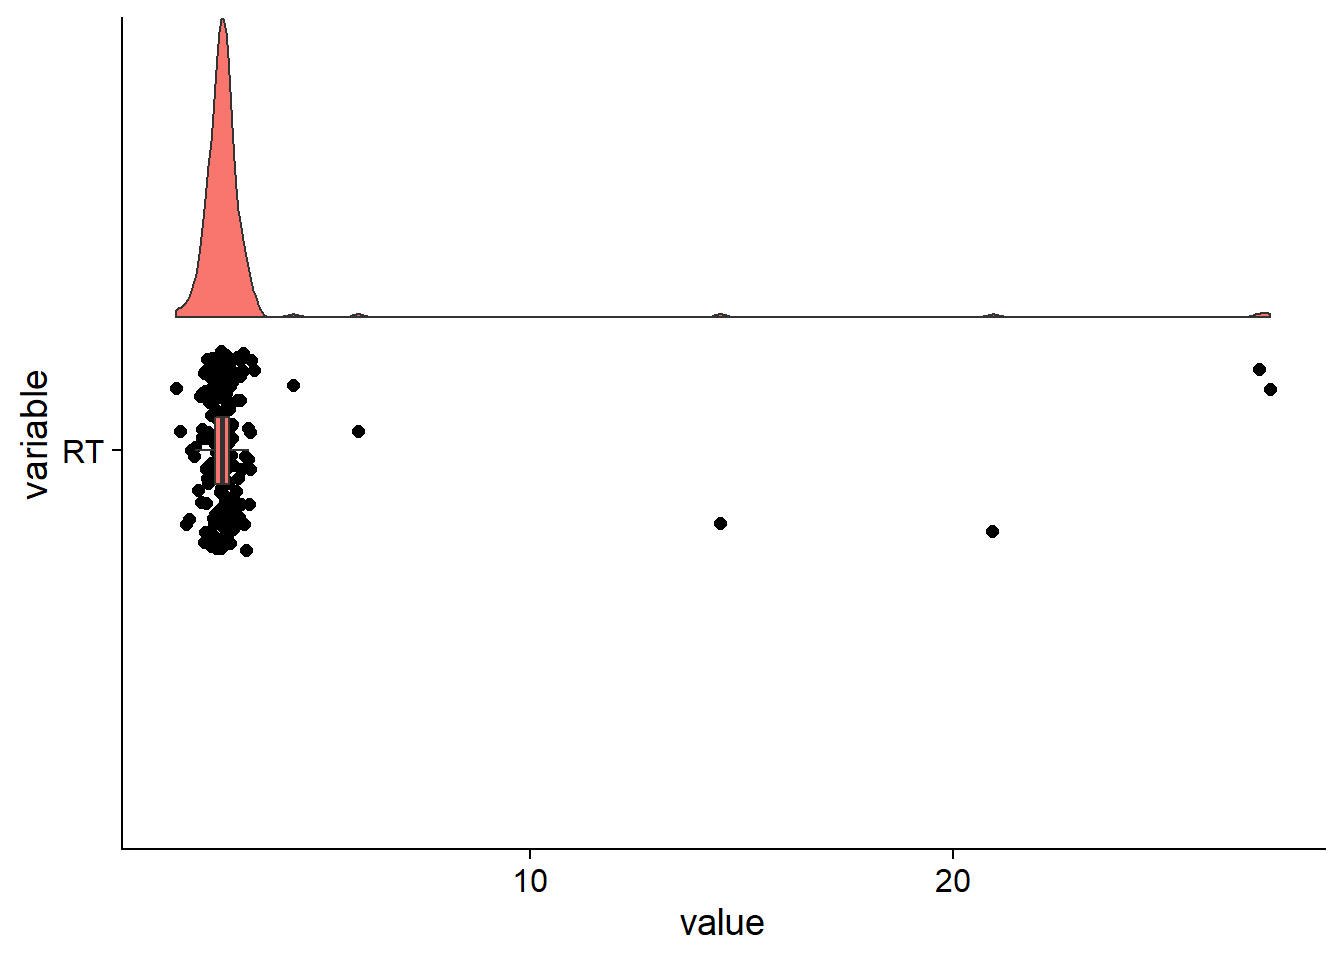
\includegraphics{ALL_TOGETHER_files/figure-latex/PVT-1}

\begin{Shaded}
\begin{Highlighting}[]
\FunctionTok{qqPlot}\NormalTok{(PVT}\SpecialCharTok{$}\NormalTok{Mean) }\CommentTok{\# clearly not a normal distribution: a big skew }
\end{Highlighting}
\end{Shaded}

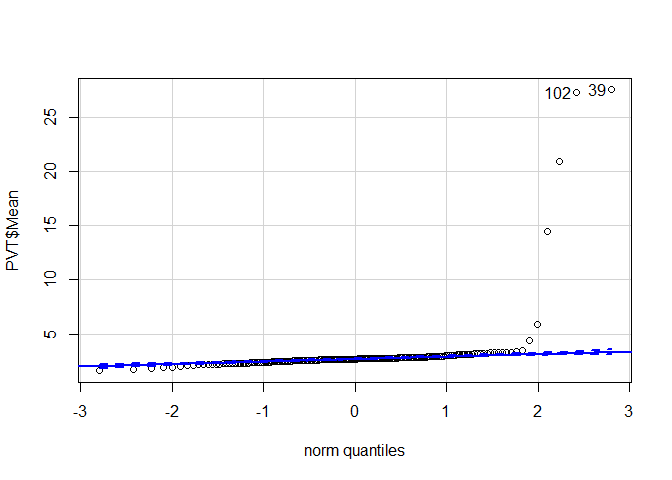
\includegraphics{ALL_TOGETHER_files/figure-latex/PVT-2}

\begin{verbatim}
## [1]  39 102
\end{verbatim}

\begin{Shaded}
\begin{Highlighting}[]
\CommentTok{\# make factors}
\NormalTok{PVT}\SpecialCharTok{$}\NormalTok{Day }\OtherTok{\textless{}{-}} \FunctionTok{factor}\NormalTok{(PVT}\SpecialCharTok{$}\NormalTok{Day)}
\NormalTok{PVT}\SpecialCharTok{$}\NormalTok{ID }\OtherTok{\textless{}{-}} \FunctionTok{factor}\NormalTok{(PVT}\SpecialCharTok{$}\NormalTok{ID)}
\NormalTok{PVT}\SpecialCharTok{$}\NormalTok{Condition }\OtherTok{\textless{}{-}} \FunctionTok{factor}\NormalTok{(PVT}\SpecialCharTok{$}\NormalTok{Condition)}


\DocumentationTok{\#\#\# CHECKING ASSUMPTIONS \#\#\#\#}
\CommentTok{\# Time x Condition 2{-}way ANOVA with interaction effect (what Borrogan did)}
\NormalTok{res.aov2 }\OtherTok{\textless{}{-}} \FunctionTok{aov}\NormalTok{(Mean }\SpecialCharTok{\textasciitilde{}}\NormalTok{ Condition }\SpecialCharTok{*}\NormalTok{ Day, }\AttributeTok{data=}\NormalTok{ PVT)}
\FunctionTok{summary}\NormalTok{(res.aov2)}\CommentTok{\# no sign! this is good, means vigilance was same in all conditions}
\end{Highlighting}
\end{Shaded}

\begin{verbatim}
##                Df Sum Sq Mean Sq F value Pr(>F)
## Condition       1    7.2   7.168   0.814  0.368
## Day             1    1.7   1.708   0.194  0.660
## Condition:Day   1    5.4   5.383   0.611  0.435
## Residuals     190 1673.4   8.807
\end{verbatim}

\begin{Shaded}
\begin{Highlighting}[]
\CommentTok{\# HOMOGENEITY OF VARIANCE}
\FunctionTok{plot}\NormalTok{(res.aov2, }\DecValTok{1}\NormalTok{) }\CommentTok{\# residuqls vs fits plot shows no evident relationship residuals and fitted values (means of groups)}
\end{Highlighting}
\end{Shaded}

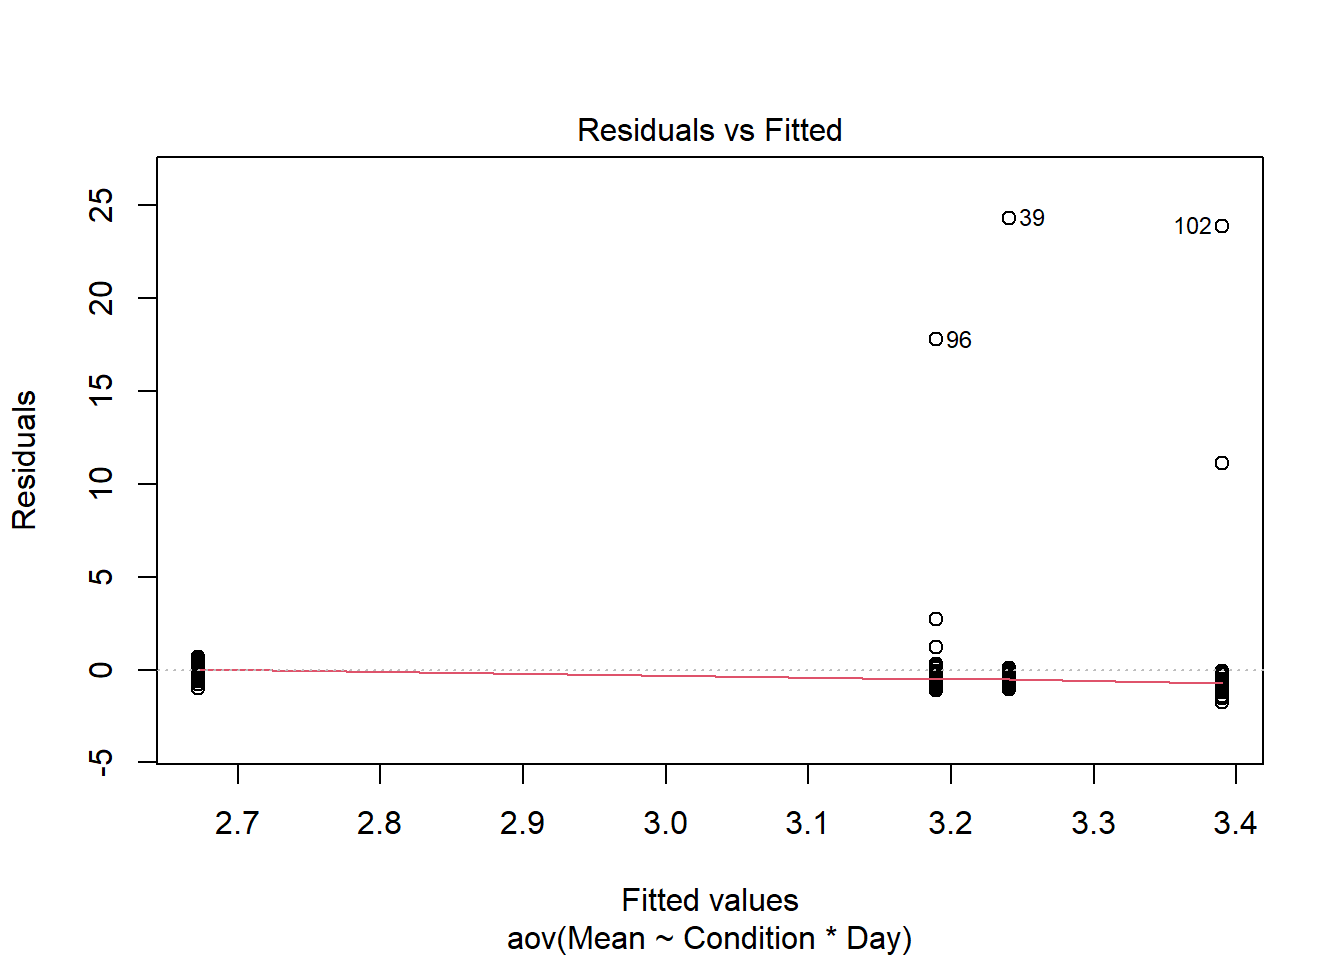
\includegraphics{ALL_TOGETHER_files/figure-latex/PVT-3}

\begin{Shaded}
\begin{Highlighting}[]
\CommentTok{\# NORMALITY}
\NormalTok{aov\_residuals }\OtherTok{\textless{}{-}} \FunctionTok{residuals}\NormalTok{ (}\AttributeTok{object=}\NormalTok{res.aov2)}
\FunctionTok{shapiro.test}\NormalTok{(}\AttributeTok{x=}\NormalTok{aov\_residuals) }\CommentTok{\# no normality! }
\end{Highlighting}
\end{Shaded}

\begin{verbatim}
## 
##  Shapiro-Wilk normality test
## 
## data:  aov_residuals
## W = 0.23635, p-value < 2.2e-16
\end{verbatim}

\begin{Shaded}
\begin{Highlighting}[]
\CommentTok{\# PVT \%\textgreater{}\%}
\CommentTok{\#   group\_by(Condition, Day) \%\textgreater{}\%}
\CommentTok{\#   shapiro.test(Mean) \# no normal distribution!}
\CommentTok{\#visualisation}
\FunctionTok{plot}\NormalTok{(res.aov2, }\DecValTok{2}\NormalTok{) }\CommentTok{\#clearly not normal}
\end{Highlighting}
\end{Shaded}

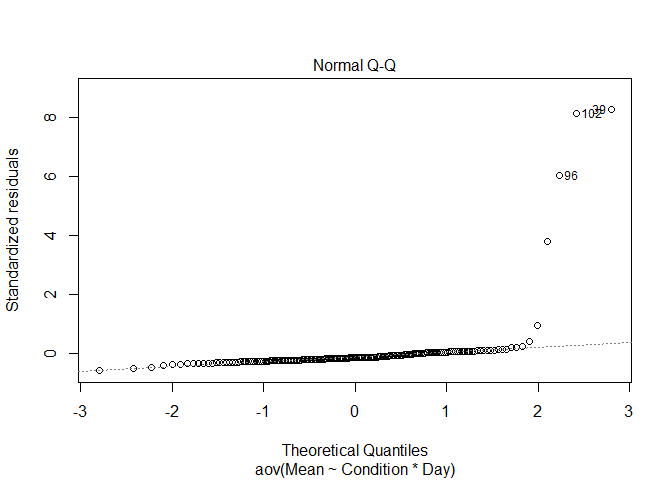
\includegraphics{ALL_TOGETHER_files/figure-latex/PVT-4}

\begin{Shaded}
\begin{Highlighting}[]
\FunctionTok{ggqqplot}\NormalTok{(PVT, }\StringTok{"Mean"}\NormalTok{, }\AttributeTok{ggtheme =} \FunctionTok{theme\_bw}\NormalTok{()) }\SpecialCharTok{+}
  \FunctionTok{facet\_grid}\NormalTok{(Day }\SpecialCharTok{\textasciitilde{}}\NormalTok{ Condition)}
\end{Highlighting}
\end{Shaded}

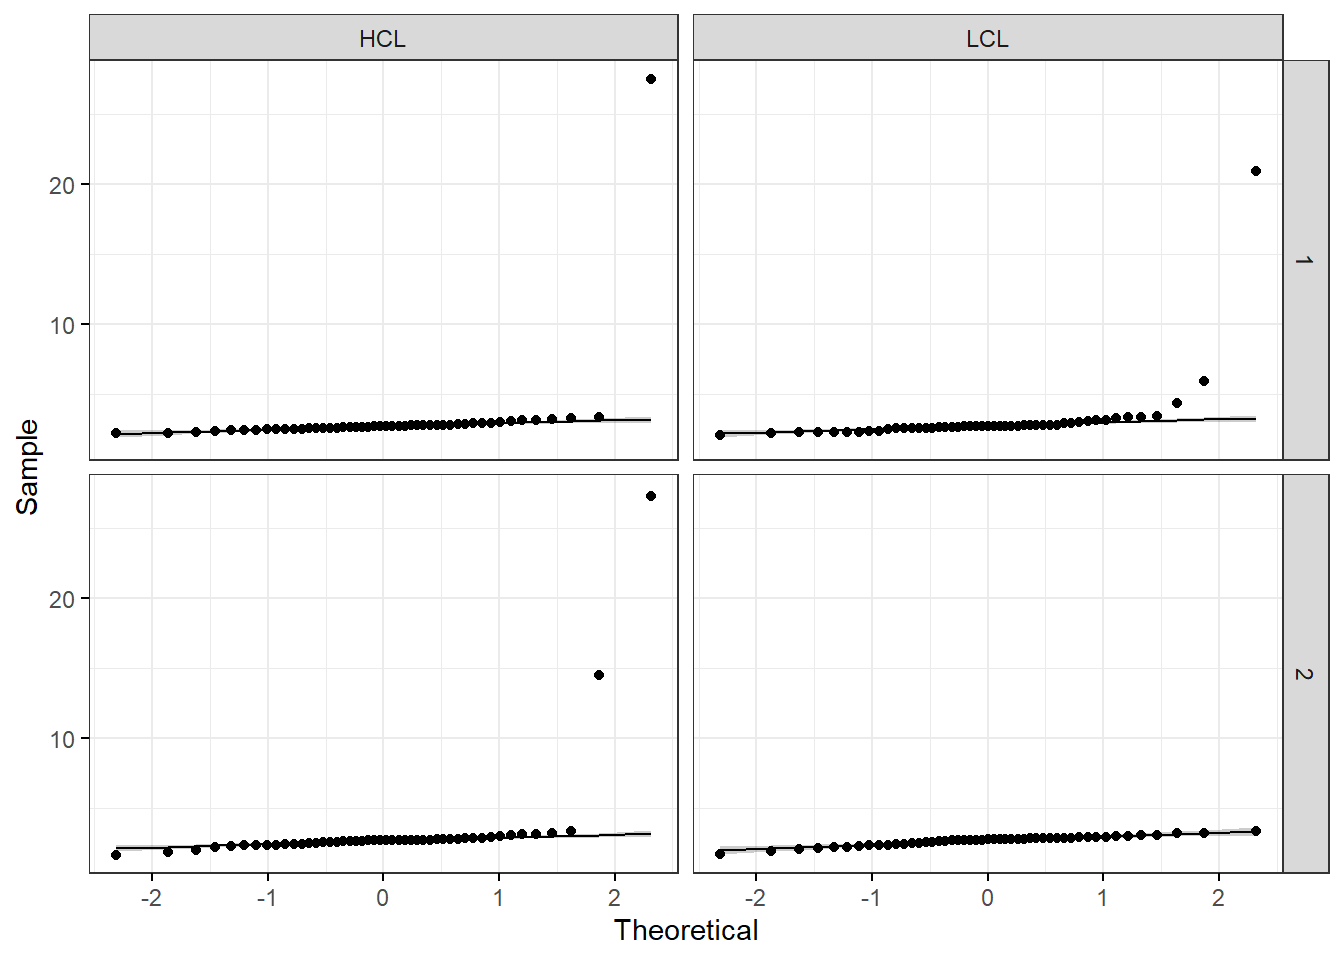
\includegraphics{ALL_TOGETHER_files/figure-latex/PVT-5}

\begin{Shaded}
\begin{Highlighting}[]
\FunctionTok{ggqqplot}\NormalTok{(PVT, }\StringTok{"Mean"}\NormalTok{, }\AttributeTok{ggtheme =} \FunctionTok{theme\_bw}\NormalTok{()) }\SpecialCharTok{+}
  \FunctionTok{facet\_grid}\NormalTok{( }\SpecialCharTok{\textasciitilde{}}\NormalTok{Condition) }\CommentTok{\#  very obviously NOT a normal distribution}
\end{Highlighting}
\end{Shaded}

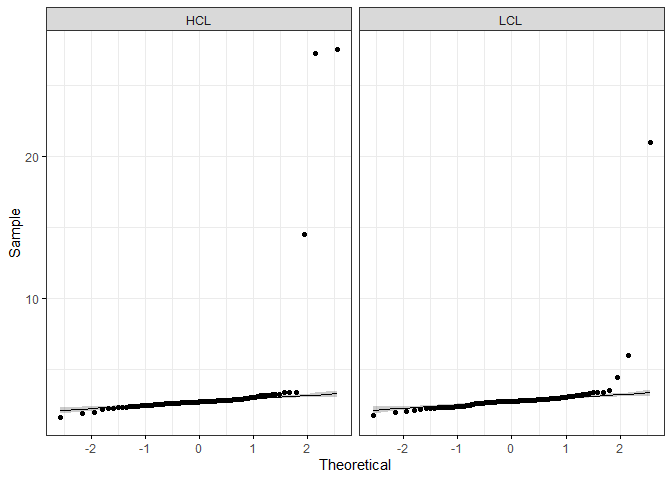
\includegraphics{ALL_TOGETHER_files/figure-latex/PVT-6}

\begin{Shaded}
\begin{Highlighting}[]
\CommentTok{\# OUTLIERS}
\FunctionTok{summary}\NormalTok{(PVT}\SpecialCharTok{$}\NormalTok{Mean)}
\end{Highlighting}
\end{Shaded}

\begin{verbatim}
##    Min. 1st Qu.  Median    Mean 3rd Qu.    Max. 
##   1.619   2.536   2.709   3.121   2.855  27.521
\end{verbatim}

\begin{Shaded}
\begin{Highlighting}[]
\NormalTok{outliers }\OtherTok{\textless{}{-}} \FunctionTok{boxplot}\NormalTok{(PVT}\SpecialCharTok{$}\NormalTok{Mean, }\AttributeTok{plot=}\ConstantTok{FALSE}\NormalTok{)}\SpecialCharTok{$}\NormalTok{out}
\CommentTok{\# remove }
\NormalTok{PVT}\OtherTok{\textless{}{-}}\NormalTok{ PVT[}\SpecialCharTok{{-}}\FunctionTok{which}\NormalTok{(PVT}\SpecialCharTok{$}\NormalTok{Mean }\SpecialCharTok{\%in\%}\NormalTok{ outliers),]}
\CommentTok{\#visualise}
\NormalTok{d}\OtherTok{\textless{}{-}}\FunctionTok{melt}\NormalTok{(}\FunctionTok{data.frame}\NormalTok{(}\AttributeTok{RT=}\FunctionTok{c}\NormalTok{(PVT}\SpecialCharTok{$}\NormalTok{Mean))) }\CommentTok{\# we melt to wide format}
\FunctionTok{distribution\_plot}\NormalTok{ (d, }\StringTok{\textquotesingle{}Mean\textquotesingle{}}\NormalTok{) }\CommentTok{\# much better}
\end{Highlighting}
\end{Shaded}

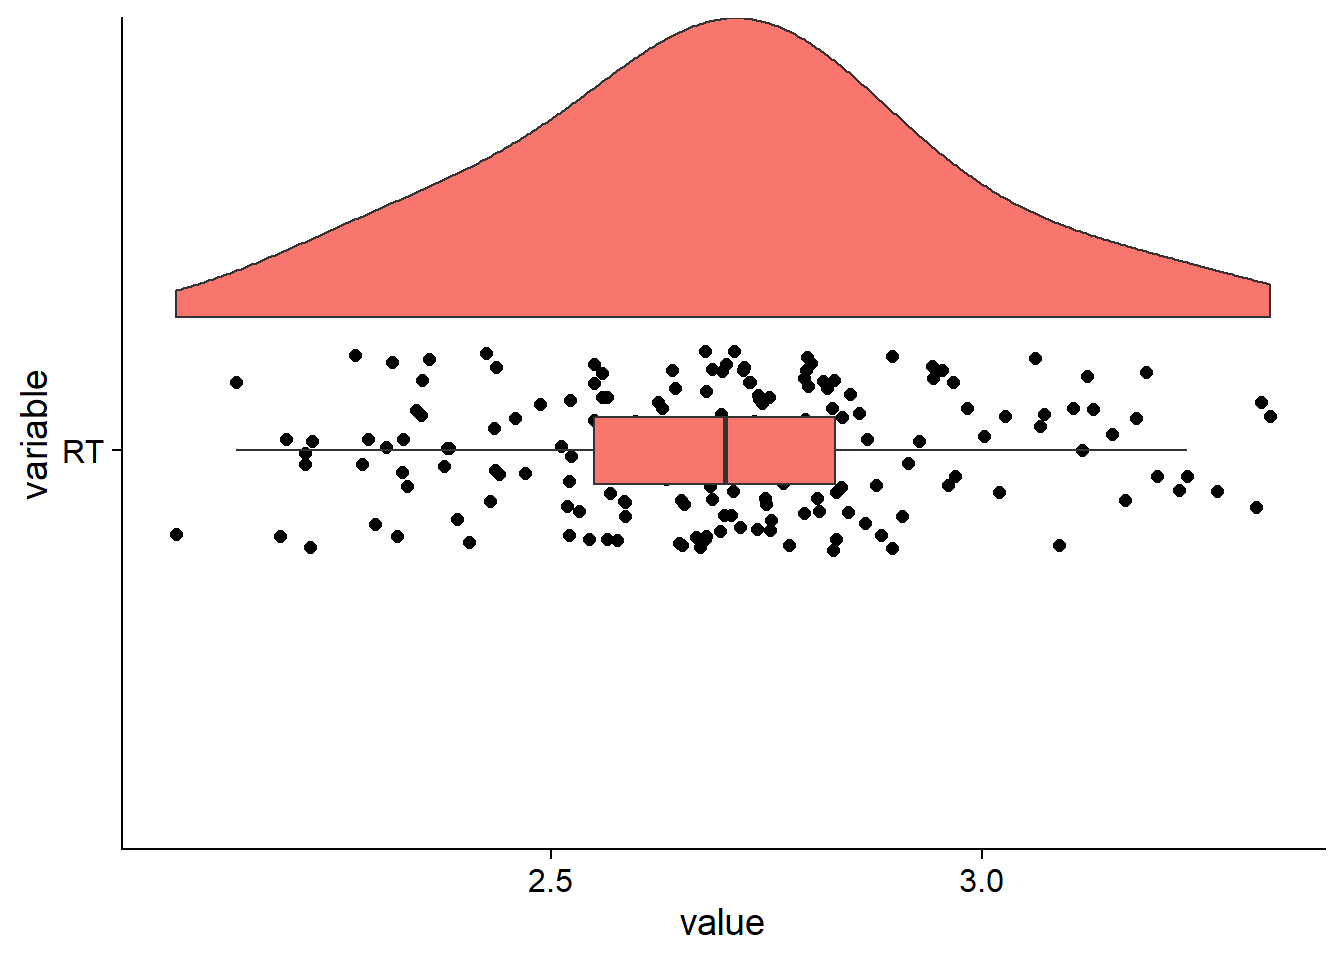
\includegraphics{ALL_TOGETHER_files/figure-latex/PVT-7}

\begin{Shaded}
\begin{Highlighting}[]
\FunctionTok{qqPlot}\NormalTok{(PVT}\SpecialCharTok{$}\NormalTok{Mean) }\CommentTok{\# much better}
\end{Highlighting}
\end{Shaded}

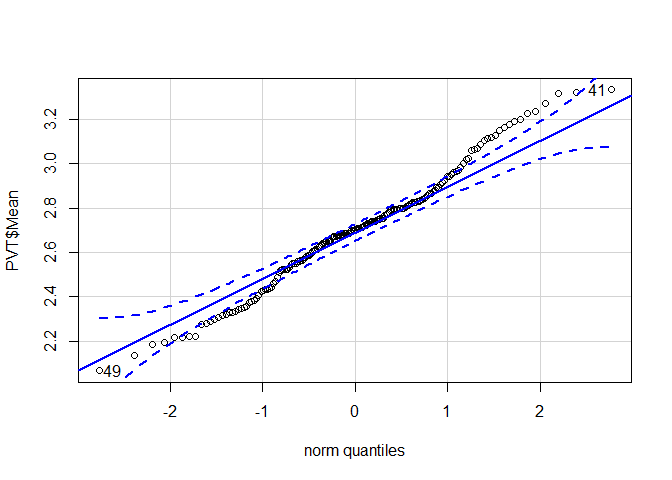
\includegraphics{ALL_TOGETHER_files/figure-latex/PVT-8}

\begin{verbatim}
## [1] 41 49
\end{verbatim}

\begin{Shaded}
\begin{Highlighting}[]
\DocumentationTok{\#\#\# ANALYSIS }\AlertTok{\#\#\#}
\CommentTok{\#https://www.frontiersin.org/articles/10.3389/fpsyg.2015.01171/full}
\CommentTok{\#https://stats.stackexchange.com/questions/254361/modeling{-}reaction{-}time{-}with{-}glmer}
\CommentTok{\# =\textgreater{} glmer with inverse link: can handle RT that is not normally distributed}
\NormalTok{d0}\FloatTok{.1} \OtherTok{\textless{}{-}} \FunctionTok{glmer}\NormalTok{ (Mean}\SpecialCharTok{\textasciitilde{}}\NormalTok{Condition }\SpecialCharTok{*}\NormalTok{ Day  }\SpecialCharTok{+}\NormalTok{ (}\DecValTok{1}\SpecialCharTok{|}\NormalTok{ID), }\AttributeTok{data=}\NormalTok{ PVT, }\AttributeTok{family=} \FunctionTok{inverse.gaussian}\NormalTok{(}\AttributeTok{link=}\StringTok{"identity"}\NormalTok{))}
\NormalTok{d0}\FloatTok{.2}\OtherTok{\textless{}{-}} \FunctionTok{glmer}\NormalTok{ (Mean}\SpecialCharTok{\textasciitilde{}}\NormalTok{Condition }\SpecialCharTok{*}\NormalTok{ Day  }\SpecialCharTok{+}\NormalTok{ (}\DecValTok{1}\SpecialCharTok{|}\NormalTok{ID), }\AttributeTok{data=}\NormalTok{ PVT, }\AttributeTok{family=}\NormalTok{ Gamma)}
\NormalTok{d0}\FloatTok{.3} \OtherTok{\textless{}{-}} \FunctionTok{glmer}\NormalTok{ (Mean}\SpecialCharTok{\textasciitilde{}}\NormalTok{Condition }\SpecialCharTok{*}\NormalTok{ Day  }\SpecialCharTok{+}\NormalTok{ (}\DecValTok{1}\SpecialCharTok{|}\NormalTok{ID), }\AttributeTok{data=}\NormalTok{ PVT, }\AttributeTok{family=}\NormalTok{ gaussian)}
\NormalTok{tabel }\OtherTok{\textless{}{-}} \FunctionTok{cbind}\NormalTok{(}\FunctionTok{AIC}\NormalTok{(d0}\FloatTok{.1}\NormalTok{, d0}\FloatTok{.2}\NormalTok{, d0}\FloatTok{.3}\NormalTok{)) }
\NormalTok{two\_w}\OtherTok{\textless{}{-}} \FunctionTok{glmer}\NormalTok{ (Mean}\SpecialCharTok{\textasciitilde{}}\NormalTok{Condition }\SpecialCharTok{*}\NormalTok{ Day  }\SpecialCharTok{+}\NormalTok{ (}\DecValTok{1}\SpecialCharTok{|}\NormalTok{ID), }\AttributeTok{data=}\NormalTok{ PVT, }\AttributeTok{family=}\NormalTok{ Gamma)}
\NormalTok{emmeans1}\OtherTok{\textless{}{-}} \FunctionTok{emmeans}\NormalTok{(two\_w, pairwise }\SpecialCharTok{\textasciitilde{}}\NormalTok{ Condition }\SpecialCharTok{*}\NormalTok{ Day, }\AttributeTok{adjust =}\StringTok{"fdr"}\NormalTok{, }\AttributeTok{type =} \StringTok{"response"}\NormalTok{)}
\NormalTok{emmean\_dataframe }\OtherTok{\textless{}{-}} \FunctionTok{summary}\NormalTok{(emmeans1)}\SpecialCharTok{$}\NormalTok{emmeans}

\FunctionTok{Anova}\NormalTok{(two\_w, }\AttributeTok{type=}\StringTok{\textquotesingle{}III\textquotesingle{}}\NormalTok{)}
\end{Highlighting}
\end{Shaded}

\begin{verbatim}
## Analysis of Deviance Table (Type III Wald chisquare tests)
## 
## Response: Mean
##                   Chisq Df Pr(>Chisq)    
## (Intercept)   2879.0223  1    < 2e-16 ***
## Condition        0.1854  1    0.66681    
## Day              5.6738  1    0.01722 *  
## Condition:Day    4.6655  1    0.03077 *  
## ---
## Signif. codes:  0 '***' 0.001 '**' 0.01 '*' 0.05 '.' 0.1 ' ' 1
\end{verbatim}

\begin{Shaded}
\begin{Highlighting}[]
\FunctionTok{summary}\NormalTok{(emmeans1) }\DocumentationTok{\#\# Result the SAME for data with or without outliers (PVT \& PVT2): because it is glmer}
\end{Highlighting}
\end{Shaded}

\begin{verbatim}
## $emmeans
##  Condition Day response     SE  df asymp.LCL asymp.UCL
##  HCL       1       2.68 0.0499 Inf      2.58      2.78
##  LCL       1       2.65 0.0491 Inf      2.56      2.75
##  HCL       2       2.61 0.0485 Inf      2.52      2.71
##  LCL       2       2.67 0.0494 Inf      2.57      2.77
## 
## Confidence level used: 0.95 
## Intervals are back-transformed from the inverse scale 
## 
## $contrasts
##  contrast      estimate      SE  df z.ratio p.value
##  HCL 1 - LCL 1 -0.00423 0.00983 Inf  -0.431  0.8002
##  HCL 1 - HCL 2 -0.00915 0.00384 Inf  -2.382  0.1033
##  HCL 1 - LCL 2 -0.00146 0.00978 Inf  -0.150  0.8811
##  LCL 1 - HCL 2 -0.00492 0.00993 Inf  -0.495  0.8002
##  LCL 1 - LCL 2  0.00277 0.00397 Inf   0.698  0.8002
##  HCL 2 - LCL 2  0.00769 0.00988 Inf   0.778  0.8002
## 
## Note: contrasts are still on the inverse scale 
## P value adjustment: fdr method for 6 tests
\end{verbatim}

\begin{Shaded}
\begin{Highlighting}[]
\CommentTok{\# but removing the outliers makes visualisations much more readable}
\CommentTok{\#summary }
\NormalTok{sum }\OtherTok{\textless{}{-}} \FunctionTok{sum\_2}\NormalTok{ (PVT, }\StringTok{\textquotesingle{}Day\textquotesingle{}}\NormalTok{, }\StringTok{\textquotesingle{}Condition\textquotesingle{}}\NormalTok{, }\StringTok{\textquotesingle{}Mean\textquotesingle{}}\NormalTok{)}
\NormalTok{sum}
\end{Highlighting}
\end{Shaded}

\begin{verbatim}
## # A tibble: 4 x 7
## # Groups:   Day [2]
##   Day   Condition     n  mean    sd     se     ic
##   <fct> <fct>     <int> <dbl> <dbl>  <dbl>  <dbl>
## 1 1     HCL          47  2.72 0.267 0.0390 0.0784
## 2 1     LCL          43  2.67 0.260 0.0396 0.0799
## 3 2     HCL          43  2.69 0.250 0.0381 0.0769
## 4 2     LCL          45  2.71 0.260 0.0388 0.0781
\end{verbatim}

\#\#\#\#VISUALISATIONS

\begin{Shaded}
\begin{Highlighting}[]
\CommentTok{\# ui\textless{}{-} fluidPage( \# makes the User Interface}
\CommentTok{\#      tabsetPanel(type = "tab",}
\CommentTok{\#                   tabPanel("bxp", plotOutput("bxp"))}
\CommentTok{\#                  \# ,}
\CommentTok{\#                  \#  tabPanel("splitviolin", plotOutput("splitviolin"))}
\CommentTok{\#          ))}
\CommentTok{\# }
\CommentTok{\# server \textless{}{-} function (input, output, session)\{ }
\CommentTok{\#   }
\CommentTok{\#    output$bxp \textless{}{-} renderPlot(\{}
\CommentTok{\#      ggboxplot(}
\CommentTok{\#       PVT, x = "Day", y = "Mean",}
\CommentTok{\#       color = "Condition", palette = "jco")}
\CommentTok{\#    \}, height=700, width=1100)}
\CommentTok{\#     }
\CommentTok{\#      \# output$splitviolin \textless{}{-} renderPlot(\{}
\CommentTok{\#      \#  plotty()(PVT, emmean\_dataframe, \textquotesingle{}Day\textquotesingle{},  \textquotesingle{}Mean\textquotesingle{}, \textquotesingle{}Condition\textquotesingle{}, \textquotesingle{}response\textquotesingle{}, \textquotesingle{}Vigilance\textquotesingle{})}
\CommentTok{\#      \#  ggsave(pl, file=paste0(plotPrefix, "PVT\_Plot.jpeg"), width = 2500, height = 1500, dpi = 300, units = "px")}
\CommentTok{\#      \# \}, height=700, width=1100)}
\CommentTok{\# }
\CommentTok{\# \}}
\CommentTok{\# shinyApp(ui=ui, server=server, options=list(height=1000))}

\DocumentationTok{\#\#\# VISUALISATION }\AlertTok{\#\#\#}
\CommentTok{\# boxplot}
\FunctionTok{ggboxplot}\NormalTok{(}
\NormalTok{  PVT, }\AttributeTok{x =} \StringTok{"Day"}\NormalTok{, }\AttributeTok{y =} \StringTok{"Mean"}\NormalTok{,}
  \AttributeTok{color =} \StringTok{"Condition"}\NormalTok{, }\AttributeTok{palette =} \StringTok{"jco"}\NormalTok{)}
\end{Highlighting}
\end{Shaded}

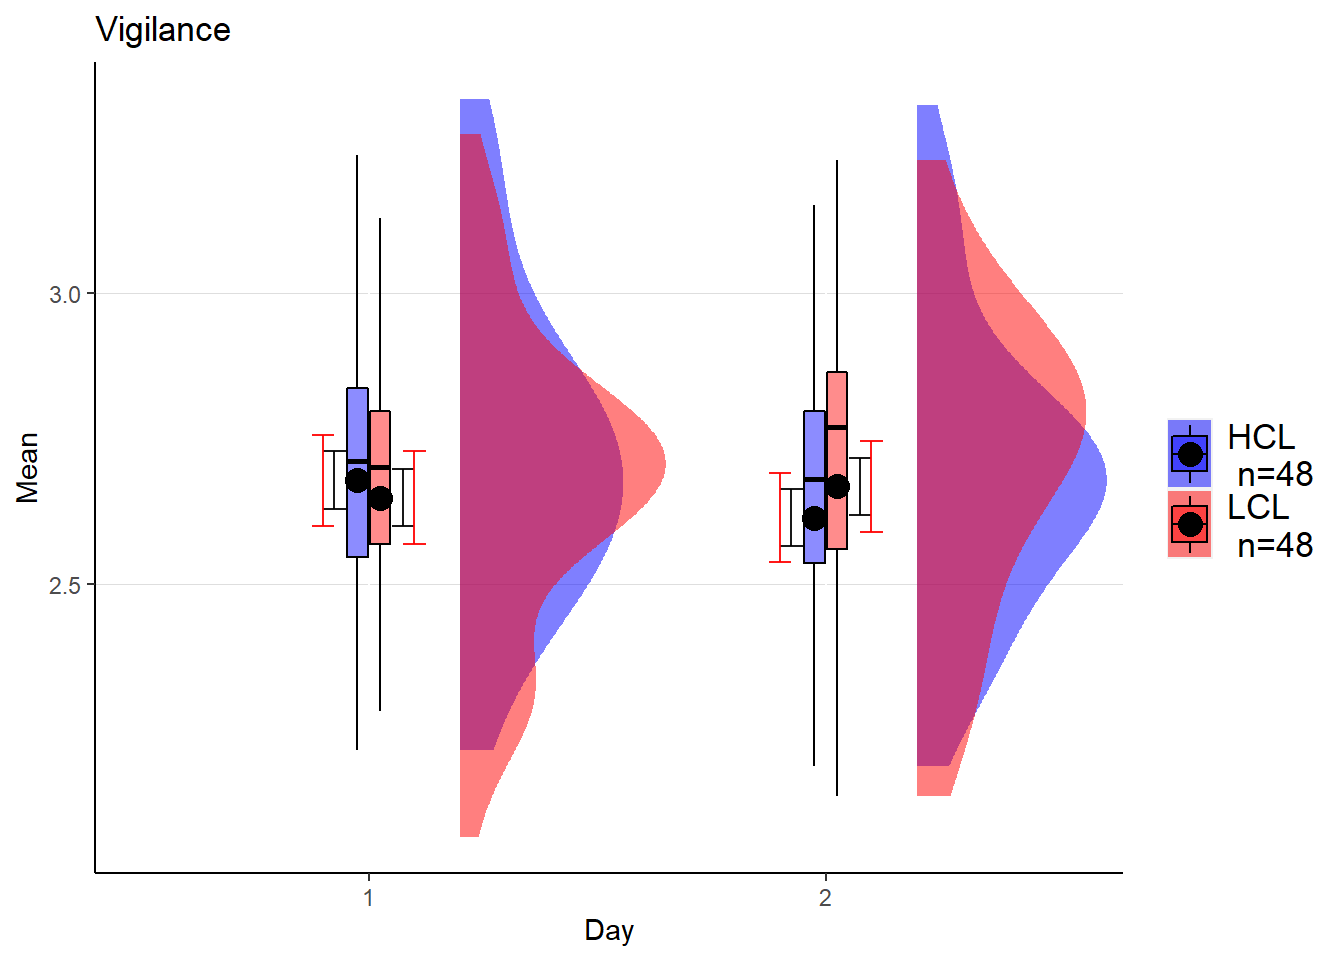
\includegraphics{ALL_TOGETHER_files/figure-latex/visualisations_PVT-1}

\begin{Shaded}
\begin{Highlighting}[]
\DocumentationTok{\#\# plot with error bars}
\NormalTok{pl }\OtherTok{\textless{}{-}} \FunctionTok{plotty}\NormalTok{(PVT, emmean\_dataframe, }\StringTok{\textquotesingle{}Day\textquotesingle{}}\NormalTok{,  }\StringTok{\textquotesingle{}Mean\textquotesingle{}}\NormalTok{, }\StringTok{\textquotesingle{}Condition\textquotesingle{}}\NormalTok{, }\StringTok{\textquotesingle{}response\textquotesingle{}}\NormalTok{, }\StringTok{\textquotesingle{}Vigilance\textquotesingle{}}\NormalTok{)}
\FunctionTok{ggsave}\NormalTok{(pl, }\AttributeTok{file=}\FunctionTok{paste0}\NormalTok{(plotPrefix, }\StringTok{"PVT\_Plot.jpeg"}\NormalTok{), }\AttributeTok{width =} \DecValTok{2500}\NormalTok{, }\AttributeTok{height =} \DecValTok{1500}\NormalTok{, }\AttributeTok{dpi =} \DecValTok{300}\NormalTok{, }\AttributeTok{units =} \StringTok{"px"}\NormalTok{)}
\NormalTok{pl}
\end{Highlighting}
\end{Shaded}

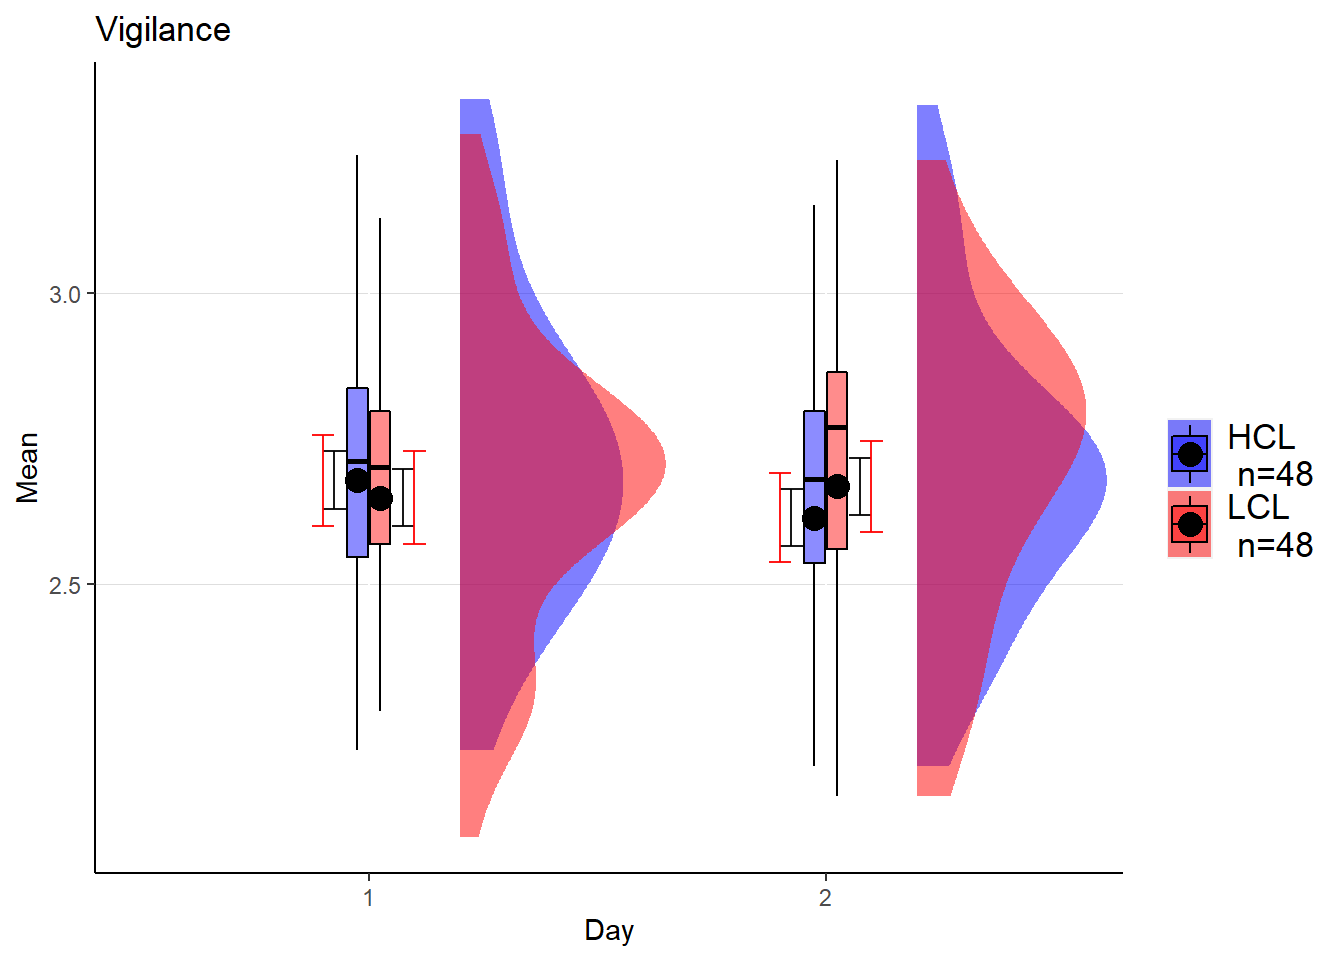
\includegraphics{ALL_TOGETHER_files/figure-latex/visualisations_PVT-2}

\hypertarget{differences}{%
\subsubsection{Differences}\label{differences}}

\begin{Shaded}
\begin{Highlighting}[]
\CommentTok{\#Download PVT data (this datafile is made in \textquotesingle{}preprocessing\textquotesingle{})}
\NormalTok{data }\OtherTok{\textless{}{-}} \FunctionTok{read.csv}\NormalTok{(}\FunctionTok{paste0}\NormalTok{(Dir, }\StringTok{"PVT.csv"}\NormalTok{), }\AttributeTok{header =} \ConstantTok{TRUE}\NormalTok{, }\AttributeTok{sep =}\NormalTok{ )}
\CommentTok{\# mean 1/RT}
\NormalTok{data}\SpecialCharTok{$}\NormalTok{RT }\OtherTok{\textless{}{-}} \DecValTok{1}\SpecialCharTok{/}\NormalTok{(data}\SpecialCharTok{$}\NormalTok{RT}\SpecialCharTok{/}\DecValTok{1000}\NormalTok{) }\CommentTok{\#1/RT  ==\textgreater{} other result}

\DocumentationTok{\#\# CREATE DATAFRAME  with the MeanRT per ID, Day, Condition}
\NormalTok{PVT }\OtherTok{\textless{}{-}} \FunctionTok{as.data.frame}\NormalTok{(}\FunctionTok{group\_by}\NormalTok{(data, Test, Day, Condition, ID) }\SpecialCharTok{\%\textgreater{}\%}
  \FunctionTok{summarise}\NormalTok{(}
    \AttributeTok{count =} \FunctionTok{n}\NormalTok{(),}
    \AttributeTok{Mean =} \FunctionTok{mean}\NormalTok{(RT, }\AttributeTok{na.rm =} \ConstantTok{TRUE}\NormalTok{)}
\NormalTok{  ))}

\CommentTok{\# visualise RT\textquotesingle{}s: from 0 to 10 seconds }
\NormalTok{d}\OtherTok{\textless{}{-}}\FunctionTok{melt}\NormalTok{(}\FunctionTok{data.frame}\NormalTok{(}\AttributeTok{RT=}\FunctionTok{c}\NormalTok{(PVT}\SpecialCharTok{$}\NormalTok{Mean))) }\CommentTok{\# we melt to wide format}
\FunctionTok{distribution\_plot}\NormalTok{ (d, }\StringTok{\textquotesingle{}Mean\textquotesingle{}}\NormalTok{)}
\end{Highlighting}
\end{Shaded}

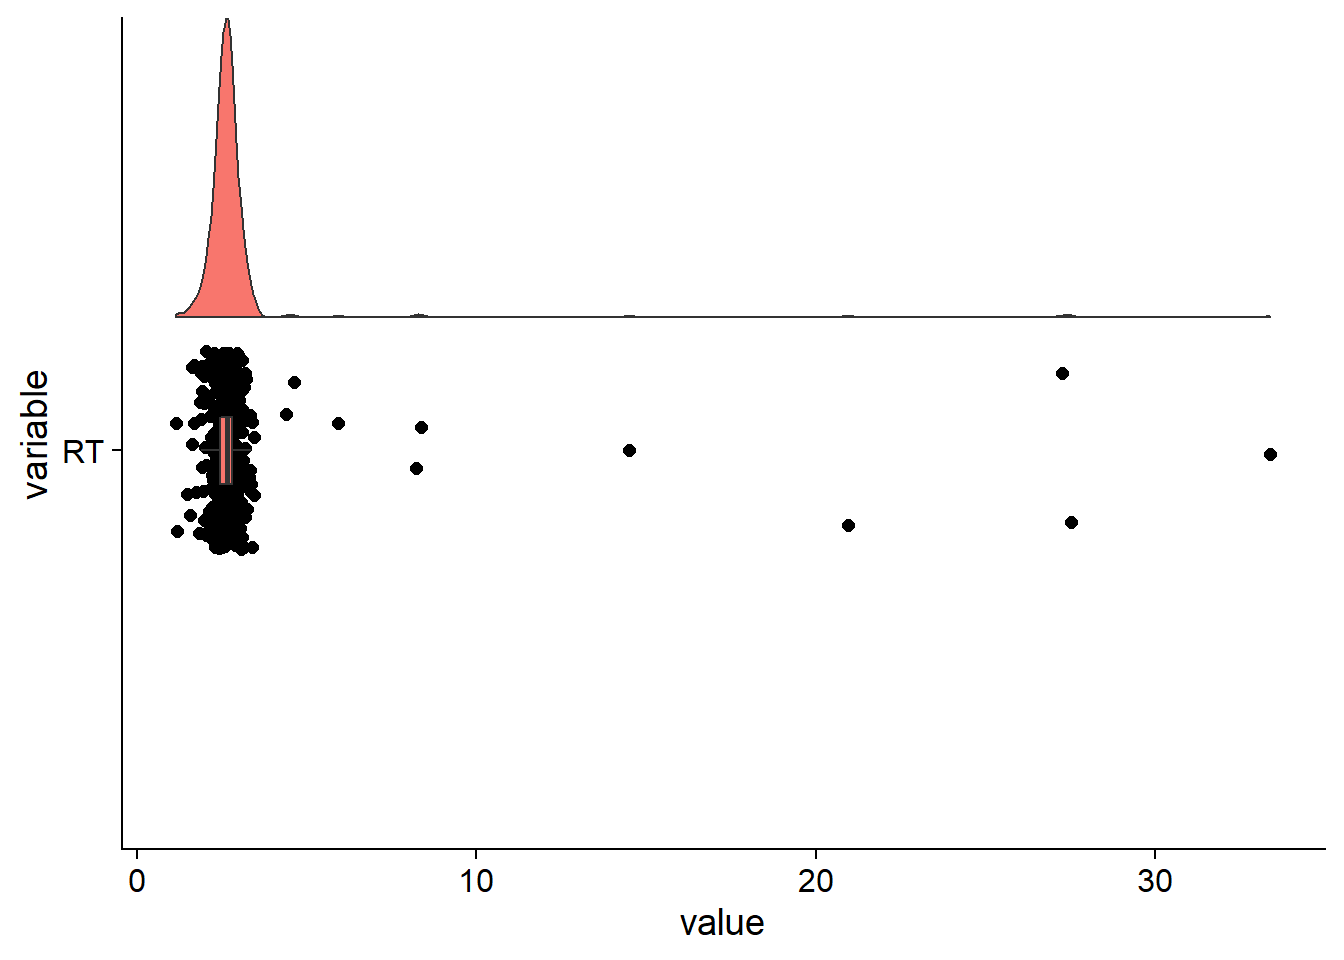
\includegraphics{ALL_TOGETHER_files/figure-latex/PVT_Differences-1}

\begin{Shaded}
\begin{Highlighting}[]
\FunctionTok{qqPlot}\NormalTok{(PVT}\SpecialCharTok{$}\NormalTok{Mean) }\CommentTok{\# clearly not a normal distribution: a big skew }
\end{Highlighting}
\end{Shaded}

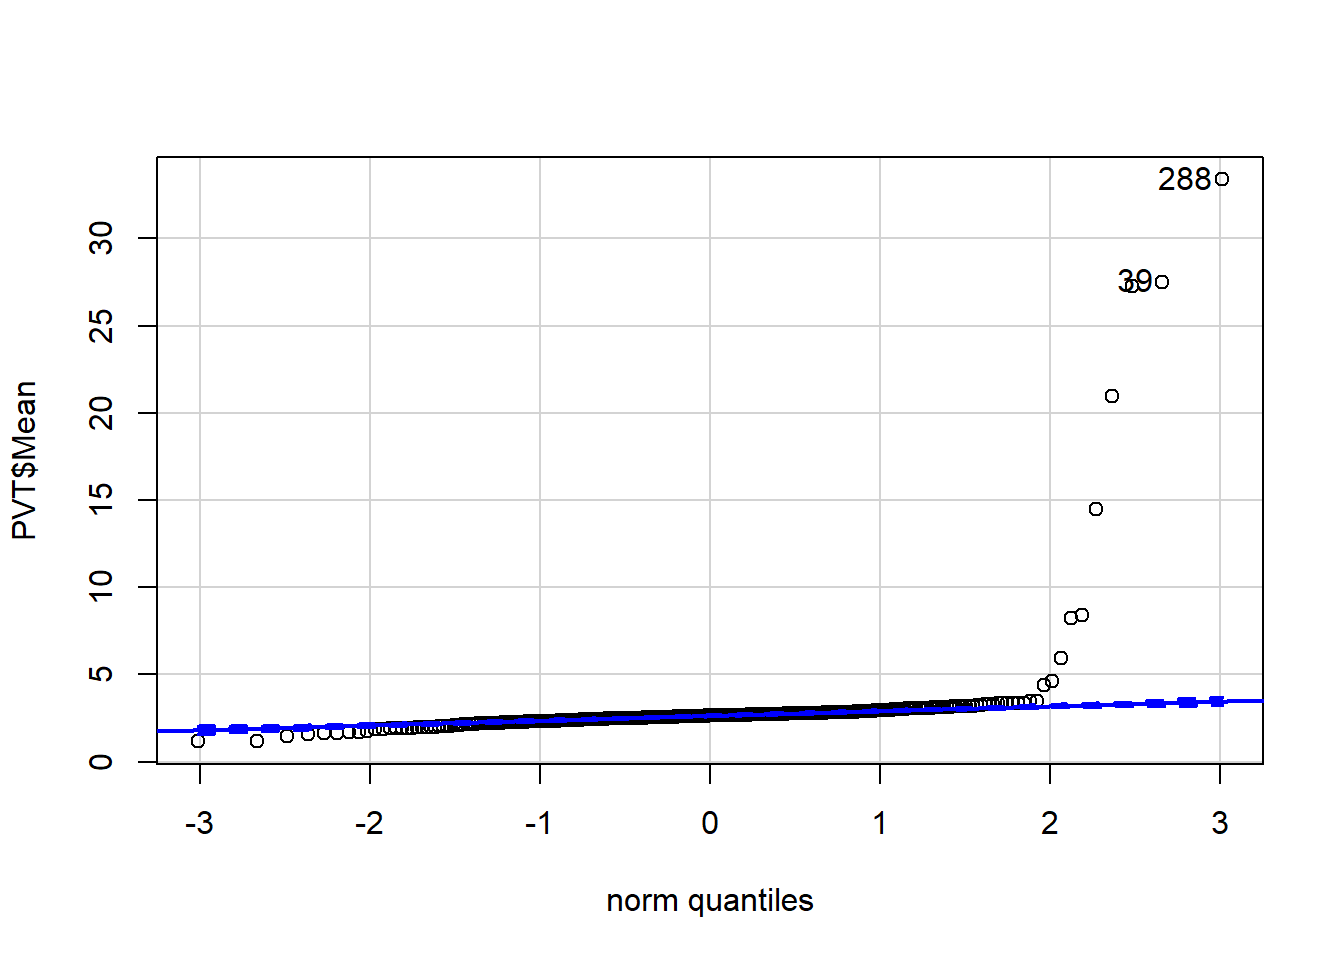
\includegraphics{ALL_TOGETHER_files/figure-latex/PVT_Differences-2}

\begin{verbatim}
## [1] 288  39
\end{verbatim}

\begin{Shaded}
\begin{Highlighting}[]
\CommentTok{\# make factors}
\NormalTok{PVT}\SpecialCharTok{$}\NormalTok{Day }\OtherTok{\textless{}{-}} \FunctionTok{factor}\NormalTok{(PVT}\SpecialCharTok{$}\NormalTok{Day)}
\NormalTok{PVT}\SpecialCharTok{$}\NormalTok{ID }\OtherTok{\textless{}{-}} \FunctionTok{factor}\NormalTok{(PVT}\SpecialCharTok{$}\NormalTok{ID)}
\NormalTok{PVT}\SpecialCharTok{$}\NormalTok{Condition }\OtherTok{\textless{}{-}} \FunctionTok{factor}\NormalTok{(PVT}\SpecialCharTok{$}\NormalTok{Condition)}
\CommentTok{\# difference score, devide by baseline (pre TloadBack) as a function of group (Day/condition): (2{-}1)/1}
\ControlFlowTok{for}\NormalTok{ (i }\ControlFlowTok{in} \DecValTok{1}\SpecialCharTok{:}\DecValTok{97}\NormalTok{) \{}
\NormalTok{  PVT}\SpecialCharTok{$}\NormalTok{Diff[PVT}\SpecialCharTok{$}\NormalTok{ID}\SpecialCharTok{==}\NormalTok{i }\SpecialCharTok{\&}\NormalTok{ PVT}\SpecialCharTok{$}\NormalTok{Day}\SpecialCharTok{==}\DecValTok{1}\NormalTok{] }\OtherTok{=}
\NormalTok{    ( ( PVT}\SpecialCharTok{$}\NormalTok{Mean[PVT}\SpecialCharTok{$}\NormalTok{Test}\SpecialCharTok{==}\DecValTok{2} \SpecialCharTok{\&}\NormalTok{ PVT}\SpecialCharTok{$}\NormalTok{ID}\SpecialCharTok{==}\NormalTok{i }\SpecialCharTok{\&}\NormalTok{ PVT}\SpecialCharTok{$}\NormalTok{Day}\SpecialCharTok{==}\DecValTok{1}\NormalTok{]}\SpecialCharTok{{-}}\NormalTok{ PVT}\SpecialCharTok{$}\NormalTok{Mean[PVT}\SpecialCharTok{$}\NormalTok{Test}\SpecialCharTok{==}\DecValTok{1} \SpecialCharTok{\&}\NormalTok{ PVT}\SpecialCharTok{$}\NormalTok{ID}\SpecialCharTok{==}\NormalTok{i }\SpecialCharTok{\&}\NormalTok{ PVT}\SpecialCharTok{$}\NormalTok{Day}\SpecialCharTok{==}\DecValTok{1}\NormalTok{] )}\SpecialCharTok{/}\NormalTok{PVT}\SpecialCharTok{$}\NormalTok{Mean[PVT}\SpecialCharTok{$}\NormalTok{Test}\SpecialCharTok{==}\DecValTok{1} \SpecialCharTok{\&}\NormalTok{ PVT}\SpecialCharTok{$}\NormalTok{ID}\SpecialCharTok{==}\NormalTok{i }\SpecialCharTok{\&}\NormalTok{ PVT}\SpecialCharTok{$}\NormalTok{Day}\SpecialCharTok{==}\DecValTok{1}\NormalTok{] )}
  
\NormalTok{  PVT}\SpecialCharTok{$}\NormalTok{Diff[PVT}\SpecialCharTok{$}\NormalTok{ID}\SpecialCharTok{==}\NormalTok{i }\SpecialCharTok{\&}\NormalTok{ PVT}\SpecialCharTok{$}\NormalTok{Day}\SpecialCharTok{==}\DecValTok{2}\NormalTok{] }\OtherTok{=}
\NormalTok{    ((PVT}\SpecialCharTok{$}\NormalTok{Mean[PVT}\SpecialCharTok{$}\NormalTok{Test}\SpecialCharTok{==}\DecValTok{2} \SpecialCharTok{\&}\NormalTok{ PVT}\SpecialCharTok{$}\NormalTok{ID}\SpecialCharTok{==}\NormalTok{i }\SpecialCharTok{\&}\NormalTok{ PVT}\SpecialCharTok{$}\NormalTok{Day}\SpecialCharTok{==}\DecValTok{2}\NormalTok{]}\SpecialCharTok{{-}}\NormalTok{ PVT}\SpecialCharTok{$}\NormalTok{Mean[PVT}\SpecialCharTok{$}\NormalTok{Test}\SpecialCharTok{==}\DecValTok{1} \SpecialCharTok{\&}\NormalTok{ PVT}\SpecialCharTok{$}\NormalTok{ID}\SpecialCharTok{==}\NormalTok{i }\SpecialCharTok{\&}\NormalTok{ PVT}\SpecialCharTok{$}\NormalTok{Day}\SpecialCharTok{==}\DecValTok{2}\NormalTok{])}\SpecialCharTok{/}\NormalTok{PVT}\SpecialCharTok{$}\NormalTok{Mean[PVT}\SpecialCharTok{$}\NormalTok{Test}\SpecialCharTok{==}\DecValTok{1} \SpecialCharTok{\&}\NormalTok{ PVT}\SpecialCharTok{$}\NormalTok{ID}\SpecialCharTok{==}\NormalTok{i }\SpecialCharTok{\&}\NormalTok{ PVT}\SpecialCharTok{$}\NormalTok{Day}\SpecialCharTok{==}\DecValTok{2}\NormalTok{])}
\NormalTok{\}}


\DocumentationTok{\#\#\# CHECKING ASSUMPTIONS \#\#\#\#}
\CommentTok{\# Time x Condition 2{-}way ANOVA with interaction effect (what Borrogan did)}
\NormalTok{res.aov2 }\OtherTok{\textless{}{-}} \FunctionTok{aov}\NormalTok{(Diff }\SpecialCharTok{\textasciitilde{}}\NormalTok{ Condition }\SpecialCharTok{*}\NormalTok{ Day, }\AttributeTok{data=}\NormalTok{ PVT)}
\FunctionTok{summary}\NormalTok{(res.aov2)}
\end{Highlighting}
\end{Shaded}

\begin{verbatim}
##                Df Sum Sq Mean Sq F value Pr(>F)
## Condition       1    2.1  2.0783   1.877  0.171
## Day             1    1.6  1.6434   1.484  0.224
## Condition:Day   1    0.7  0.7349   0.664  0.416
## Residuals     384  425.1  1.1071
\end{verbatim}

\begin{Shaded}
\begin{Highlighting}[]
\CommentTok{\# HOMOGENEITY OF VARIANCE}
\FunctionTok{plot}\NormalTok{(res.aov2, }\DecValTok{1}\NormalTok{) }\CommentTok{\# residuqls vs fits plot shows no evident relationship residuals and fitted values (Diffs of groups)}
\end{Highlighting}
\end{Shaded}

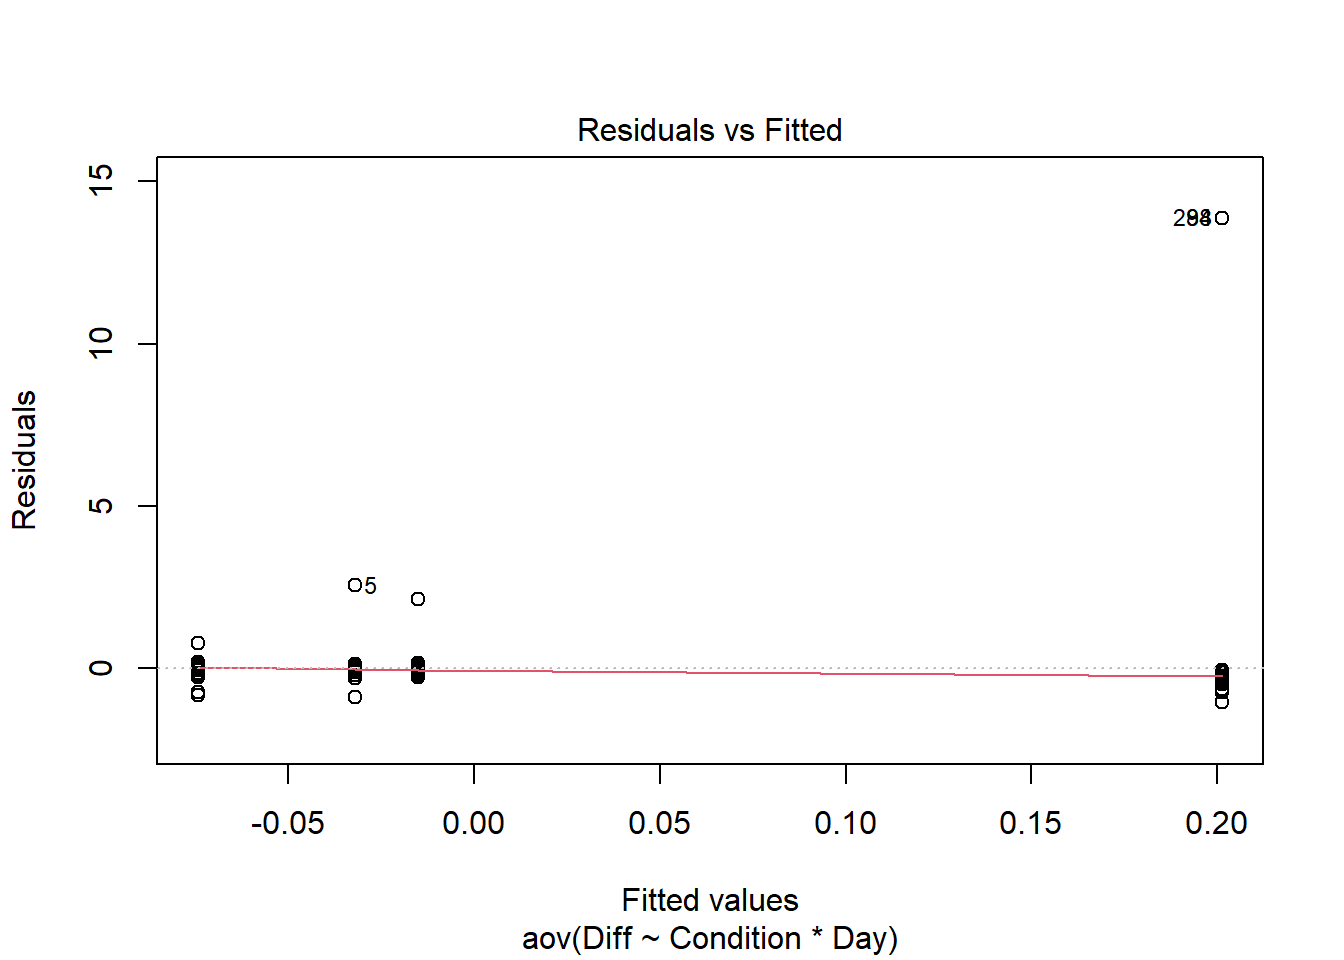
\includegraphics{ALL_TOGETHER_files/figure-latex/PVT_Differences-3}

\begin{Shaded}
\begin{Highlighting}[]
\CommentTok{\# NORMALITY}
\NormalTok{aov\_residuals }\OtherTok{\textless{}{-}} \FunctionTok{residuals}\NormalTok{ (}\AttributeTok{object=}\NormalTok{res.aov2)}
\FunctionTok{shapiro.test}\NormalTok{(}\AttributeTok{x=}\NormalTok{aov\_residuals) }\CommentTok{\#}
\end{Highlighting}
\end{Shaded}

\begin{verbatim}
## 
##  Shapiro-Wilk normality test
## 
## data:  aov_residuals
## W = 0.17526, p-value < 2.2e-16
\end{verbatim}

\begin{Shaded}
\begin{Highlighting}[]
\NormalTok{PVT }\SpecialCharTok{\%\textgreater{}\%}
  \FunctionTok{group\_by}\NormalTok{(Condition, Day) }\SpecialCharTok{\%\textgreater{}\%}
  \FunctionTok{shapiro\_test}\NormalTok{(Diff) }\CommentTok{\#}
\end{Highlighting}
\end{Shaded}

\begin{verbatim}
## # A tibble: 4 x 5
##   Day   Condition variable statistic        p
##   <fct> <fct>     <chr>        <dbl>    <dbl>
## 1 1     HCL       Diff         0.368 2.02e-18
## 2 2     HCL       Diff         0.648 7.92e-14
## 3 1     LCL       Diff         0.174 5.89e-21
## 4 2     LCL       Diff         0.360 1.04e-18
\end{verbatim}

\begin{Shaded}
\begin{Highlighting}[]
\CommentTok{\#visualisation}
\FunctionTok{plot}\NormalTok{(res.aov2, }\DecValTok{2}\NormalTok{) }\CommentTok{\#normal}
\end{Highlighting}
\end{Shaded}

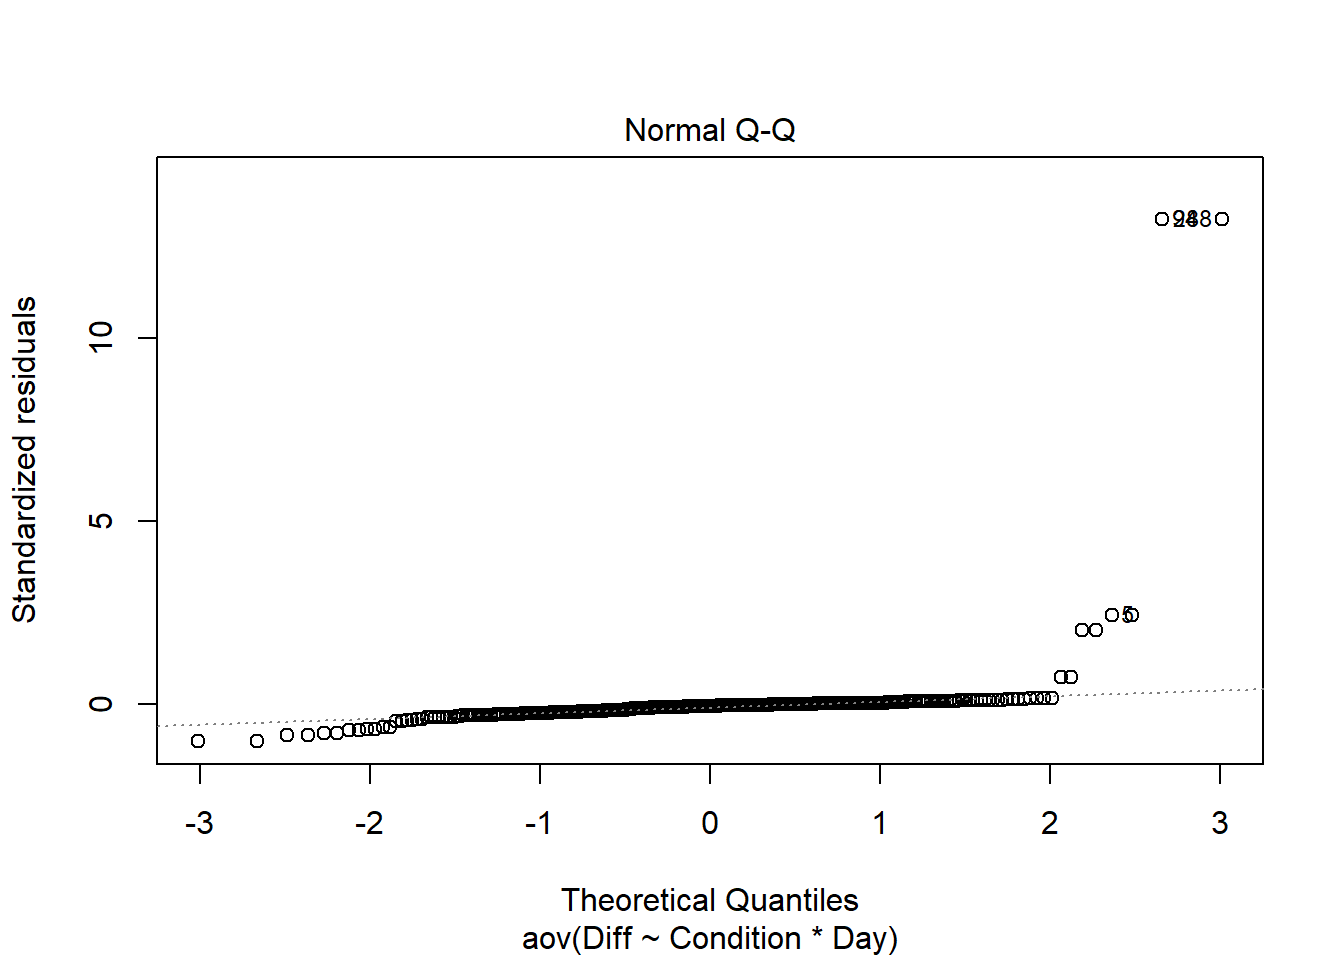
\includegraphics{ALL_TOGETHER_files/figure-latex/PVT_Differences-4}

\begin{Shaded}
\begin{Highlighting}[]
\FunctionTok{ggqqplot}\NormalTok{(PVT, }\StringTok{"Diff"}\NormalTok{, }\AttributeTok{ggtheme =} \FunctionTok{theme\_bw}\NormalTok{()) }\SpecialCharTok{+}
  \FunctionTok{facet\_grid}\NormalTok{(Day }\SpecialCharTok{\textasciitilde{}}\NormalTok{ Condition)}
\end{Highlighting}
\end{Shaded}

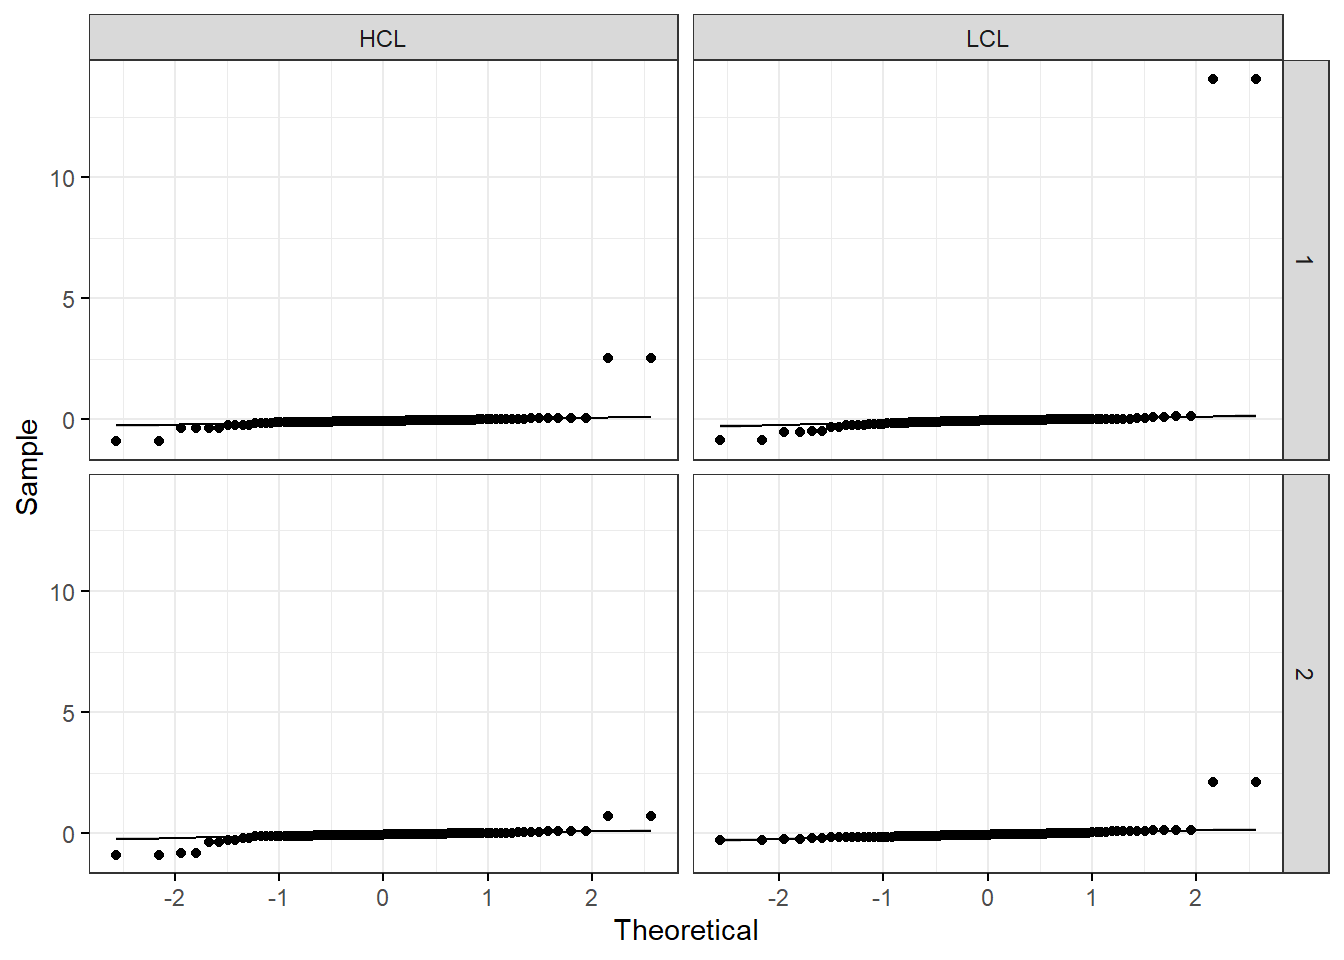
\includegraphics{ALL_TOGETHER_files/figure-latex/PVT_Differences-5}

\begin{Shaded}
\begin{Highlighting}[]
\FunctionTok{ggqqplot}\NormalTok{(PVT, }\StringTok{"Diff"}\NormalTok{, }\AttributeTok{ggtheme =} \FunctionTok{theme\_bw}\NormalTok{()) }\SpecialCharTok{+}
  \FunctionTok{facet\_grid}\NormalTok{( }\SpecialCharTok{\textasciitilde{}}\NormalTok{Condition) }\CommentTok{\#  very obviously NOT a normal distribution}
\end{Highlighting}
\end{Shaded}

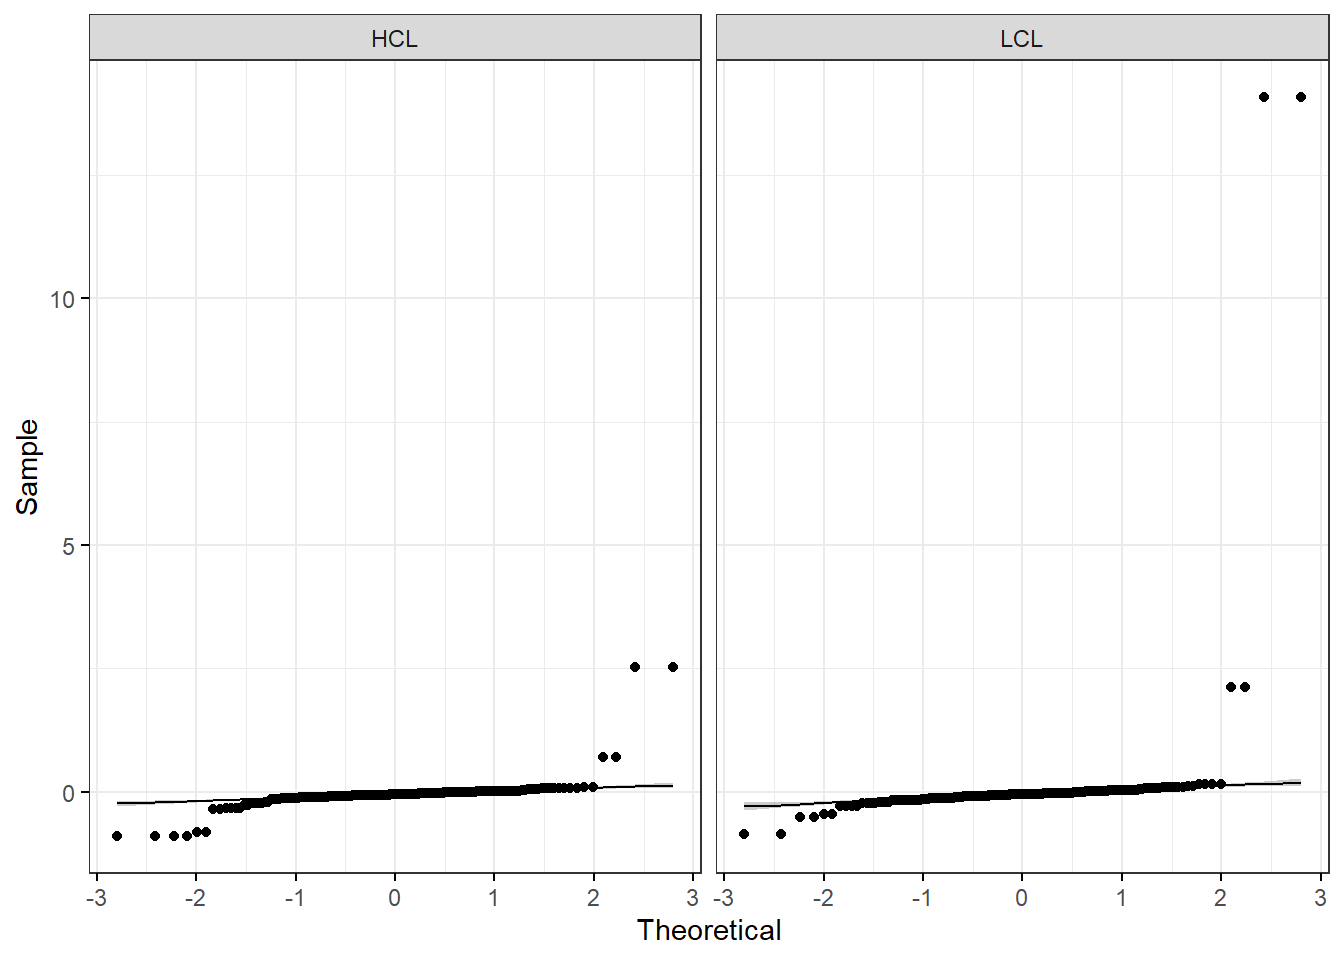
\includegraphics{ALL_TOGETHER_files/figure-latex/PVT_Differences-6}

\begin{Shaded}
\begin{Highlighting}[]
\CommentTok{\# SPHERICITY: Mauchly\textquotesingle{}s test}
\NormalTok{x}\OtherTok{\textless{}{-}}\FunctionTok{anova\_test}\NormalTok{(}\AttributeTok{data=}\NormalTok{ PVT, }\AttributeTok{dv=}\NormalTok{ Diff, }\AttributeTok{wid=}\NormalTok{ ID, }\AttributeTok{between=}\NormalTok{ Condition, }\AttributeTok{within=} \FunctionTok{c}\NormalTok{(Test, Day))}
\FunctionTok{get\_anova\_table}\NormalTok{(x, }\AttributeTok{correction =} \FunctionTok{c}\NormalTok{(}\StringTok{\textquotesingle{}GG\textquotesingle{}}\NormalTok{)) }\CommentTok{\#variances are NOT equal!}
\end{Highlighting}
\end{Shaded}

\begin{verbatim}
## ANOVA Table (type III tests)
## 
##               Effect DFn DFd     F     p p<.05      ges
## 1          Condition   1  95 0.980 0.325       5.00e-03
## 2               Test   1  95   NaN   NaN  <NA> 0.00e+00
## 3                Day   1  95 0.688 0.409       4.00e-03
## 4     Condition:Test   1  95   Inf 0.000     * 6.87e-37
## 5      Condition:Day   1  95 0.312 0.578       2.00e-03
## 6           Test:Day   1  95   Inf 0.000     * 2.75e-36
## 7 Condition:Test:Day   1  95   Inf 0.000     * 6.87e-37
\end{verbatim}

\begin{Shaded}
\begin{Highlighting}[]
\NormalTok{x}\SpecialCharTok{$}\StringTok{\textquotesingle{}Sphericity Corrections\textquotesingle{}}
\end{Highlighting}
\end{Shaded}

\begin{verbatim}
## NULL
\end{verbatim}

\begin{Shaded}
\begin{Highlighting}[]
\CommentTok{\# OUTLIERS}
\FunctionTok{summary}\NormalTok{(PVT}\SpecialCharTok{$}\NormalTok{Diff)}
\end{Highlighting}
\end{Shaded}

\begin{verbatim}
##      Min.   1st Qu.    Median      Mean   3rd Qu.      Max. 
## -0.910595 -0.108391 -0.053066  0.020690 -0.001091 14.071161
\end{verbatim}

\begin{Shaded}
\begin{Highlighting}[]
\NormalTok{outliers }\OtherTok{\textless{}{-}} \FunctionTok{boxplot}\NormalTok{(PVT}\SpecialCharTok{$}\NormalTok{Diff, }\AttributeTok{plot=}\ConstantTok{FALSE}\NormalTok{)}\SpecialCharTok{$}\NormalTok{out}
\CommentTok{\# remove}
\NormalTok{ PVT}\OtherTok{\textless{}{-}}\NormalTok{ PVT[}\SpecialCharTok{{-}}\FunctionTok{which}\NormalTok{(PVT}\SpecialCharTok{$}\NormalTok{Diff }\SpecialCharTok{\%in\%}\NormalTok{ outliers),]}
\CommentTok{\#visualise}
\NormalTok{d}\OtherTok{\textless{}{-}}\FunctionTok{melt}\NormalTok{(}\FunctionTok{data.frame}\NormalTok{(}\AttributeTok{PVT=}\FunctionTok{c}\NormalTok{(PVT}\SpecialCharTok{$}\NormalTok{Diff))) }\CommentTok{\# we melt to wide format}
\FunctionTok{distribution\_plot}\NormalTok{ (d, }\StringTok{\textquotesingle{}Diff\textquotesingle{}}\NormalTok{)}
\end{Highlighting}
\end{Shaded}

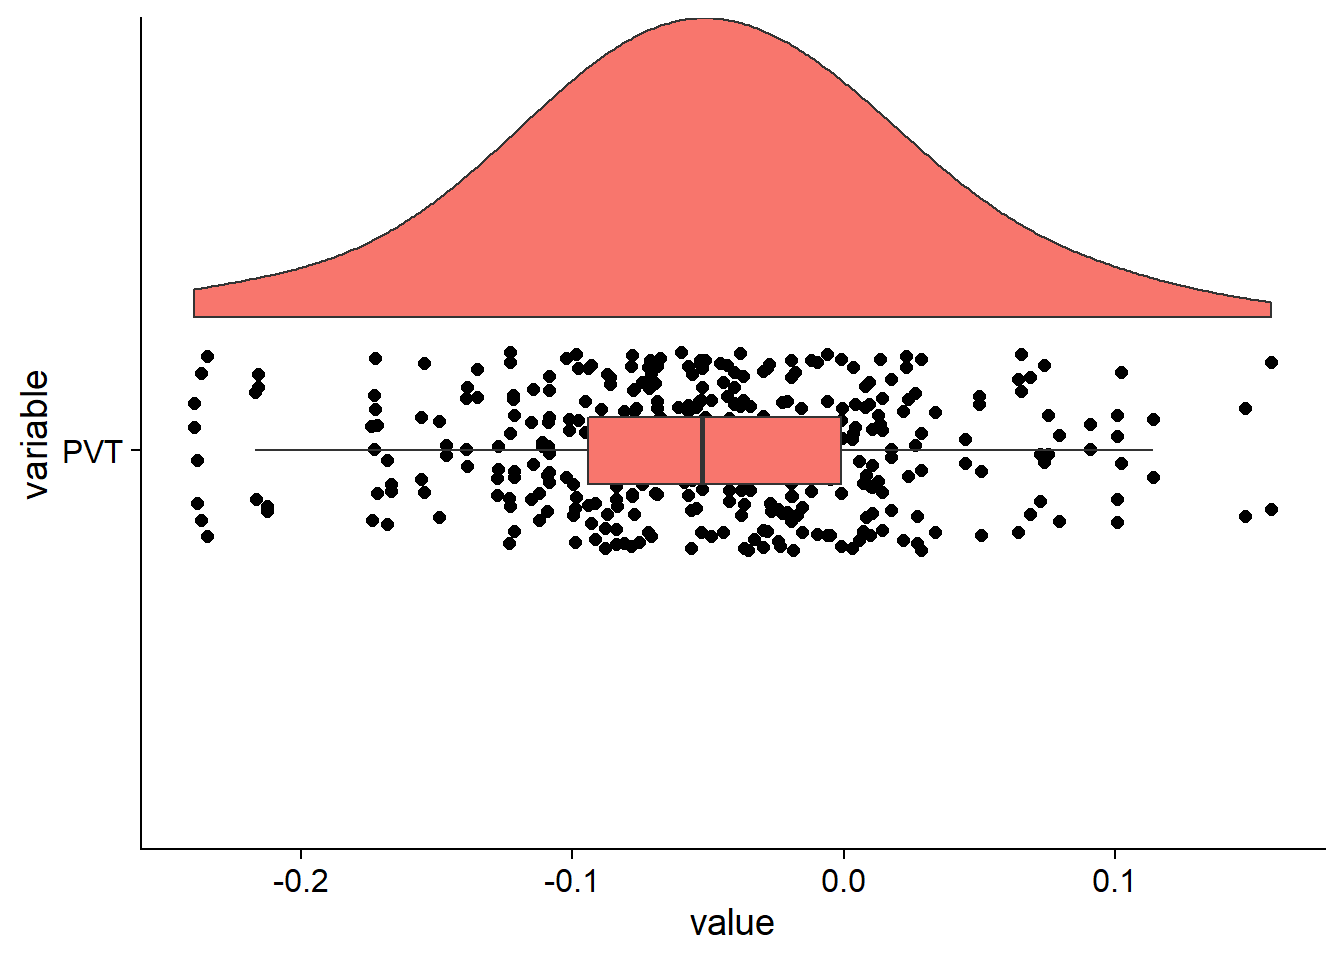
\includegraphics{ALL_TOGETHER_files/figure-latex/PVT_Differences-7}

\begin{Shaded}
\begin{Highlighting}[]
\FunctionTok{qqPlot}\NormalTok{(PVT}\SpecialCharTok{$}\NormalTok{Diff)}
\end{Highlighting}
\end{Shaded}

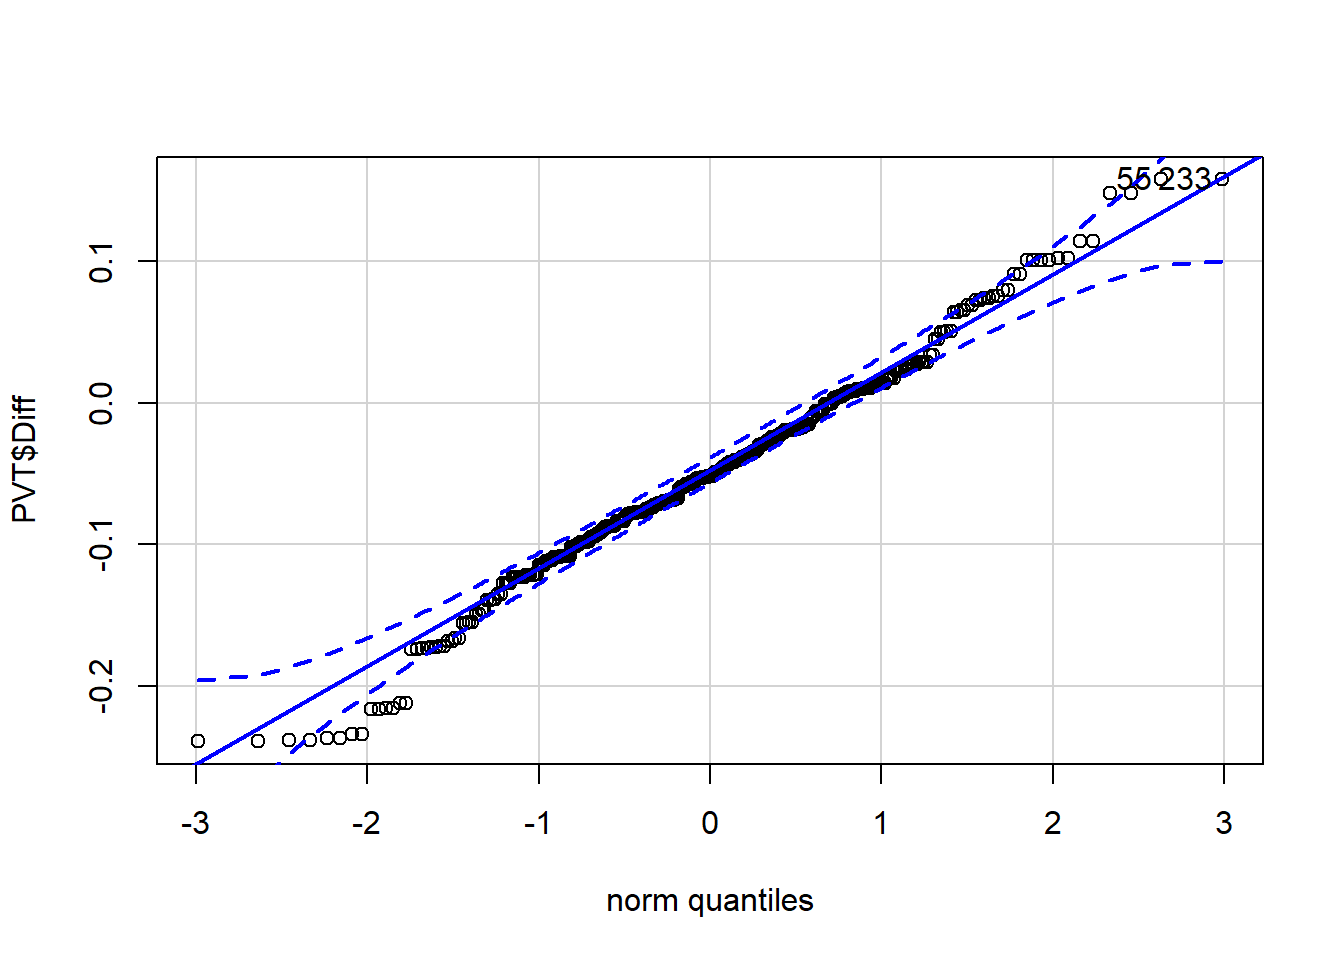
\includegraphics{ALL_TOGETHER_files/figure-latex/PVT_Differences-8}

\begin{verbatim}
## [1]  55 233
\end{verbatim}

\begin{Shaded}
\begin{Highlighting}[]
\NormalTok{res.aov2 }\OtherTok{\textless{}{-}} \FunctionTok{aov}\NormalTok{(Diff }\SpecialCharTok{\textasciitilde{}}\NormalTok{ Condition }\SpecialCharTok{*}\NormalTok{ Day, }\AttributeTok{data=}\NormalTok{ PVT)}
\CommentTok{\# HOMOGENEITY OF VARIANCE}
\FunctionTok{plot}\NormalTok{(res.aov2, }\DecValTok{1}\NormalTok{) }\CommentTok{\# residuqls vs fits plot shows no evident relationship residuals and fitted values (Diffs of groups)}
\end{Highlighting}
\end{Shaded}

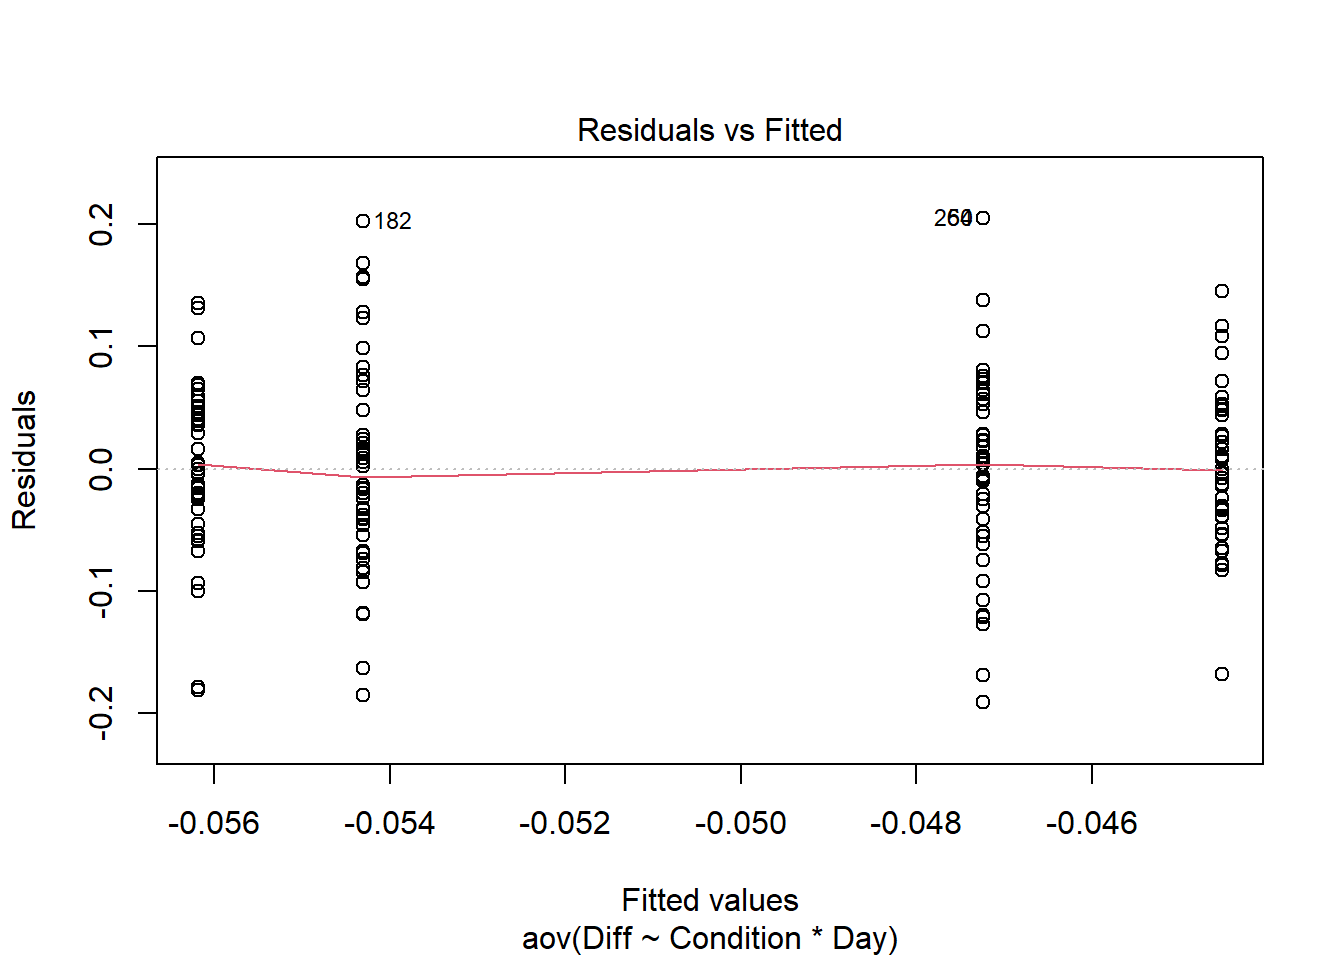
\includegraphics{ALL_TOGETHER_files/figure-latex/PVT_Differences-9}

\begin{Shaded}
\begin{Highlighting}[]
\CommentTok{\# NORMALITY}
\NormalTok{aov\_residuals }\OtherTok{\textless{}{-}} \FunctionTok{residuals}\NormalTok{ (}\AttributeTok{object=}\NormalTok{res.aov2)}
\FunctionTok{shapiro.test}\NormalTok{(}\AttributeTok{x=}\NormalTok{aov\_residuals) }
\end{Highlighting}
\end{Shaded}

\begin{verbatim}
## 
##  Shapiro-Wilk normality test
## 
## data:  aov_residuals
## W = 0.98878, p-value = 0.007709
\end{verbatim}

\begin{Shaded}
\begin{Highlighting}[]
\DocumentationTok{\#\#\#\# repeated{-}measures ANOVA \#\#\#\#}
\NormalTok{x}\OtherTok{\textless{}{-}}\FunctionTok{anova\_test}\NormalTok{(}\AttributeTok{data=}\NormalTok{ PVT, }\AttributeTok{dv=}\NormalTok{ Diff, }\AttributeTok{wid=}\NormalTok{ ID, }\AttributeTok{between=}\NormalTok{ Condition, }\AttributeTok{within=} \FunctionTok{c}\NormalTok{(Test, Day))}
\FunctionTok{get\_anova\_table}\NormalTok{(x)}
\end{Highlighting}
\end{Shaded}

\begin{verbatim}
## ANOVA Table (type III tests)
## 
##               Effect DFn DFd     F     p p<.05      ges
## 1          Condition   1  81 0.003 0.959       1.82e-05
## 2               Test   1  81   Inf 0.000     * 5.89e-34
## 3                Day   1  81 0.014 0.905       7.90e-05
## 4     Condition:Test   1  81   NaN   NaN  <NA> 0.00e+00
## 5      Condition:Day   1  81 1.490 0.226       8.00e-03
## 6           Test:Day   1  81   NaN   NaN  <NA> 0.00e+00
## 7 Condition:Test:Day   1  81   Inf 0.000     * 9.21e-36
\end{verbatim}

\begin{Shaded}
\begin{Highlighting}[]
\CommentTok{\#tukey\textquotesingle{}s post{-}hoc analyses: see if performance decreased faster in HCL compared to LCL}
\NormalTok{two\_w }\OtherTok{\textless{}{-}} \FunctionTok{lm}\NormalTok{(Diff }\SpecialCharTok{\textasciitilde{}}\NormalTok{ Test}\SpecialCharTok{*}\NormalTok{Condition, }\AttributeTok{data=}\NormalTok{ PVT)}
\NormalTok{emmeans1}\OtherTok{\textless{}{-}} \FunctionTok{emmeans}\NormalTok{(two\_w, pairwise }\SpecialCharTok{\textasciitilde{}}\NormalTok{ Test}\SpecialCharTok{*}\NormalTok{Condition, }\AttributeTok{adjust =}\StringTok{"fdr"}\NormalTok{, }\AttributeTok{type =} \StringTok{"response"}\NormalTok{)}
\NormalTok{emDiff\_dataframe }\OtherTok{\textless{}{-}} \FunctionTok{summary}\NormalTok{(emmeans1)}\SpecialCharTok{$}\NormalTok{emmeans}
\FunctionTok{Anova}\NormalTok{(two\_w, }\AttributeTok{type=}\StringTok{\textquotesingle{}III\textquotesingle{}}\NormalTok{)}
\end{Highlighting}
\end{Shaded}

\begin{verbatim}
## Anova Table (Type III tests)
## 
## Response: Diff
##                 Sum Sq  Df F value   Pr(>F)   
## (Intercept)    0.04423   1  8.0383 0.004844 **
## Test           0.00000   1  0.0000 1.000000   
## Condition      0.00000   1  0.0004 0.984962   
## Test:Condition 0.00000   1  0.0000 1.000000   
## Residuals      1.93700 352                    
## ---
## Signif. codes:  0 '***' 0.001 '**' 0.01 '*' 0.05 '.' 0.1 ' ' 1
\end{verbatim}

\begin{Shaded}
\begin{Highlighting}[]
\FunctionTok{summary}\NormalTok{(emmeans1)}
\end{Highlighting}
\end{Shaded}

\begin{verbatim}
## $emmeans
##  Test Condition  emmean      SE  df lower.CL upper.CL
##     1 HCL       -0.0504 0.00795 352  -0.0661  -0.0348
##     2 HCL       -0.0504 0.00795 352  -0.0661  -0.0348
##     1 LCL       -0.0509 0.00778 352  -0.0662  -0.0356
##     2 LCL       -0.0509 0.00778 352  -0.0662  -0.0356
## 
## Confidence level used: 0.95 
## 
## $contrasts
##  contrast      estimate     SE  df t.ratio p.value
##  1 HCL - 2 HCL 0.000000 0.0112 352   0.000  1.0000
##  1 HCL - 1 LCL 0.000469 0.0111 352   0.042  1.0000
##  1 HCL - 2 LCL 0.000469 0.0111 352   0.042  1.0000
##  2 HCL - 1 LCL 0.000469 0.0111 352   0.042  1.0000
##  2 HCL - 2 LCL 0.000469 0.0111 352   0.042  1.0000
##  1 LCL - 2 LCL 0.000000 0.0110 352   0.000  1.0000
## 
## P value adjustment: fdr method for 6 tests
\end{verbatim}

\begin{Shaded}
\begin{Highlighting}[]
\CommentTok{\#summary}
\NormalTok{sum }\OtherTok{\textless{}{-}} \FunctionTok{sum\_3}\NormalTok{ (PVT, }\StringTok{\textquotesingle{}Test\textquotesingle{}}\NormalTok{, }\StringTok{\textquotesingle{}Condition\textquotesingle{}}\NormalTok{, }\StringTok{\textquotesingle{}Day\textquotesingle{}}\NormalTok{, }\StringTok{\textquotesingle{}Diff\textquotesingle{}}\NormalTok{)}
\NormalTok{sum}
\end{Highlighting}
\end{Shaded}

\begin{verbatim}
## # A tibble: 8 x 8
## # Groups:   Test, Condition [4]
##    Test Condition Day       n    mean     sd      se     ic
##   <int> <fct>     <fct> <int>   <dbl>  <dbl>   <dbl>  <dbl>
## 1     1 HCL       1        44 -0.0562 0.0672 0.0101  0.0204
## 2     1 HCL       2        43 -0.0445 0.0608 0.00927 0.0187
## 3     1 LCL       1        44 -0.0472 0.0794 0.0120  0.0241
## 4     1 LCL       2        47 -0.0543 0.0865 0.0126  0.0254
## 5     2 HCL       1        44 -0.0562 0.0672 0.0101  0.0204
## 6     2 HCL       2        43 -0.0445 0.0608 0.00927 0.0187
## 7     2 LCL       1        44 -0.0472 0.0794 0.0120  0.0241
## 8     2 LCL       2        47 -0.0543 0.0865 0.0126  0.0254
\end{verbatim}

\begin{Shaded}
\begin{Highlighting}[]
\DocumentationTok{\#\# VISUALISATION}
\CommentTok{\# boxplot}
\NormalTok{bxp }\OtherTok{\textless{}{-}} \FunctionTok{ggboxplot}\NormalTok{(}
\NormalTok{  PVT, }\AttributeTok{x =} \StringTok{"Condition"}\NormalTok{, }\AttributeTok{y =} \StringTok{"Diff"}\NormalTok{,}
  \AttributeTok{color =} \StringTok{"Test"}\NormalTok{, }\AttributeTok{palette =} \StringTok{"jco"}\NormalTok{,}
  \AttributeTok{facet.by =} \StringTok{"Day"}\NormalTok{, }\AttributeTok{short.panel.labs =} \ConstantTok{FALSE}
\NormalTok{  )}
\NormalTok{bxp}
\end{Highlighting}
\end{Shaded}

\hypertarget{section}{%
\subsection{\texorpdfstring{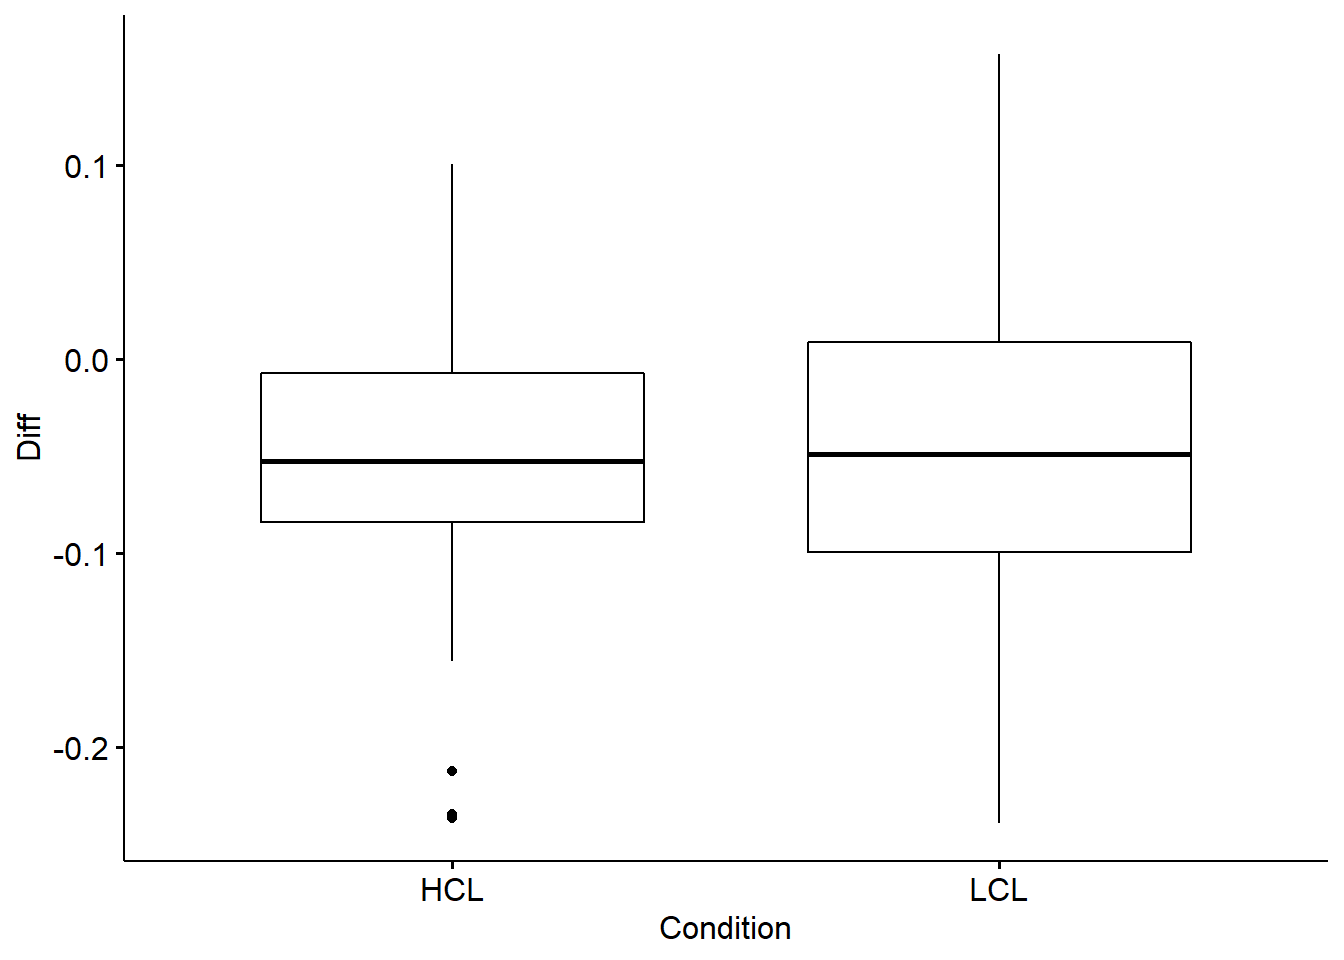
\includegraphics{ALL_TOGETHER_files/figure-latex/PVT_Differences-10}}{}}\label{section}}

\hypertarget{subjective-cf-vas-f}{%
\subsection{Subjective CF: VAS-f}\label{subjective-cf-vas-f}}

= subjective measure of fatigue on 1-10 scale we want to know if there
is a difference in VAS before and after Test

\begin{Shaded}
\begin{Highlighting}[]
\DocumentationTok{\#\#\#\#\#\#\#\#\#\#\#\#\#\#\#\#\#\#\#\#\#\#\#\#\#\#\#\#\#\#\#\#\#\#\#\#\#\#\#\#\#\#}
  \DocumentationTok{\#\#\# VAS{-}f: fatigue }\AlertTok{\#\#\#}
\DocumentationTok{\#\#\#\#\#\#\#\#\#\#\#\#\#\#\#\#\#\#\#\#\#\#\#\#\#\#\#\#\#\#\#\#\#\#\#\#\#\#\#\#\#}

\DocumentationTok{\#\#\#\# DOWNLOAD + CLEAN DATA \#\#\#\#}
\NormalTok{data }\OtherTok{\textless{}{-}} \FunctionTok{read.csv}\NormalTok{(}\FunctionTok{paste0}\NormalTok{(Dir, }\StringTok{"VAS.csv"}\NormalTok{), }\AttributeTok{header =} \ConstantTok{TRUE}\NormalTok{, }\AttributeTok{sep =}\NormalTok{ )}
\NormalTok{data }\OtherTok{\textless{}{-}}\NormalTok{data[(}\FunctionTok{grepl}\NormalTok{(}\StringTok{"quantised"}\NormalTok{, data}\SpecialCharTok{$}\NormalTok{Question.Key)),] }\CommentTok{\#VAS has \textquotesingle{}quantised: 1{-}11 instead of 0{-}10}
\CommentTok{\# create dataframe}
\NormalTok{VAS }\OtherTok{\textless{}{-}} \FunctionTok{as.data.frame}\NormalTok{(}\FunctionTok{group\_by}\NormalTok{(data, Test, Day, Condition, ID) }\SpecialCharTok{\%\textgreater{}\%}
  \FunctionTok{summarise}\NormalTok{(}
    \AttributeTok{count =} \FunctionTok{n}\NormalTok{(),}
    \AttributeTok{Mean =} \FunctionTok{mean}\NormalTok{(Response, }\AttributeTok{na.rm =} \ConstantTok{TRUE}\NormalTok{)}
\NormalTok{  )) }\CommentTok{\# we do Mean instead of Difference 2{-}1/1. Reason: this led to non{-}normal data}


\CommentTok{\#factors}
\NormalTok{VAS}\SpecialCharTok{$}\NormalTok{Day }\OtherTok{\textless{}{-}} \FunctionTok{as.factor}\NormalTok{(VAS}\SpecialCharTok{$}\NormalTok{Day)}
\NormalTok{VAS}\SpecialCharTok{$}\NormalTok{Condition }\OtherTok{\textless{}{-}} \FunctionTok{as.factor}\NormalTok{(VAS}\SpecialCharTok{$}\NormalTok{Condition)}
\NormalTok{VAS}\SpecialCharTok{$}\NormalTok{ID }\OtherTok{\textless{}{-}} \FunctionTok{as.factor}\NormalTok{(VAS}\SpecialCharTok{$}\NormalTok{ID)}
\FunctionTok{names}\NormalTok{(VAS)[}\FunctionTok{names}\NormalTok{(VAS)}\SpecialCharTok{==}\StringTok{"Test"}\NormalTok{] }\OtherTok{\textless{}{-}} \StringTok{"Time"}
\NormalTok{VAS}\SpecialCharTok{$}\NormalTok{Time }\OtherTok{\textless{}{-}} \FunctionTok{as.factor}\NormalTok{(VAS}\SpecialCharTok{$}\NormalTok{Time)}

\DocumentationTok{\#\#\# CHECKING ASSUMPTIONS \#\#\#\#}
\CommentTok{\# Time x Condition 2{-}way ANOVA with interaction effect (what Borrogan did)}
\NormalTok{res.aov2 }\OtherTok{\textless{}{-}} \FunctionTok{aov}\NormalTok{(Mean }\SpecialCharTok{\textasciitilde{}}\NormalTok{ Condition }\SpecialCharTok{*}\NormalTok{ Day, }\AttributeTok{data=}\NormalTok{ VAS)}
\FunctionTok{summary}\NormalTok{(res.aov2)}\CommentTok{\# no sign! this is good, means vigilance was same in all conditions}
\end{Highlighting}
\end{Shaded}

\begin{verbatim}
##                Df Sum Sq Mean Sq F value  Pr(>F)   
## Condition       1    9.4   9.406   3.304 0.06990 . 
## Day             1   26.3  26.291   9.235 0.00254 **
## Condition:Day   1    0.5   0.498   0.175 0.67604   
## Residuals     384 1093.2   2.847                   
## ---
## Signif. codes:  0 '***' 0.001 '**' 0.01 '*' 0.05 '.' 0.1 ' ' 1
\end{verbatim}

\begin{Shaded}
\begin{Highlighting}[]
\CommentTok{\# HOMOGENEITY OF VARIANCE}
\FunctionTok{leveneTest}\NormalTok{(Mean}\SpecialCharTok{\textasciitilde{}}\NormalTok{ Time }\SpecialCharTok{*}\NormalTok{ Condition, }\AttributeTok{data=}\NormalTok{ VAS) }\CommentTok{\# no homogeneity! problem! }
\end{Highlighting}
\end{Shaded}

\begin{verbatim}
## Levene's Test for Homogeneity of Variance (center = median)
##        Df F value Pr(>F)
## group   3  1.5305 0.2061
##       384
\end{verbatim}

\begin{Shaded}
\begin{Highlighting}[]
\CommentTok{\# box\_m(VAS[, \textquotesingle{}Mean\textquotesingle{}, drop=FALSE], VAS$Condition) }
\FunctionTok{plot}\NormalTok{(res.aov2, }\DecValTok{1}\NormalTok{) }\CommentTok{\# residuqls vs fits plot shows no evident relationship residuals and fitted values (means of groups)}
\end{Highlighting}
\end{Shaded}

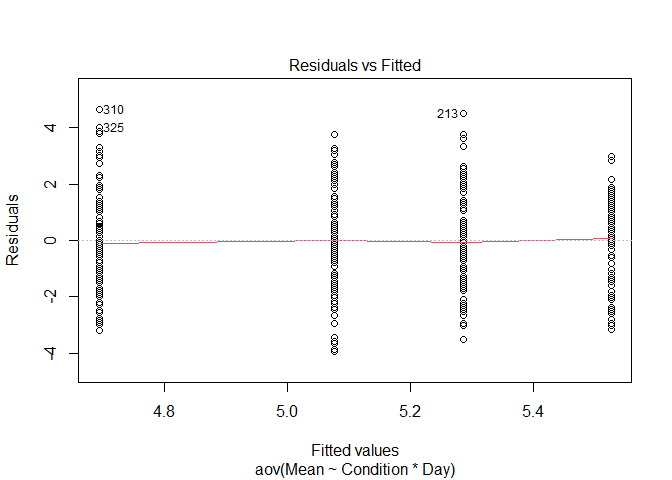
\includegraphics{ALL_TOGETHER_files/figure-latex/VASf-1}

\begin{Shaded}
\begin{Highlighting}[]
\CommentTok{\# NORMALITY}
\NormalTok{aov\_residuals }\OtherTok{\textless{}{-}} \FunctionTok{residuals}\NormalTok{ (}\AttributeTok{object=}\NormalTok{res.aov2)}
\FunctionTok{shapiro.test}\NormalTok{(}\AttributeTok{x=}\NormalTok{aov\_residuals) }\CommentTok{\#  }
\end{Highlighting}
\end{Shaded}

\begin{verbatim}
## 
##  Shapiro-Wilk normality test
## 
## data:  aov_residuals
## W = 0.99501, p-value = 0.2453
\end{verbatim}

\begin{Shaded}
\begin{Highlighting}[]
\CommentTok{\# VAS \%\textgreater{}\%}
\CommentTok{\#   group\_by(Condition, Day) \%\textgreater{}\%}
\CommentTok{\#   shapiro.test(Mean) \# }
\CommentTok{\#visualisation}
\FunctionTok{plot}\NormalTok{(res.aov2, }\DecValTok{2}\NormalTok{) }\CommentTok{\#normal}
\end{Highlighting}
\end{Shaded}

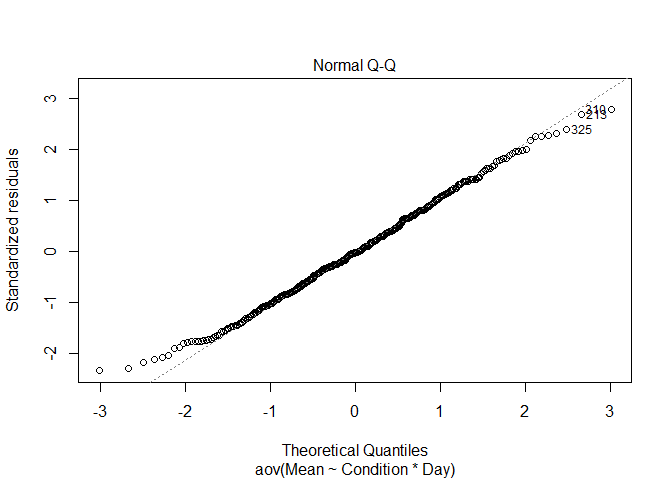
\includegraphics{ALL_TOGETHER_files/figure-latex/VASf-2}

\begin{Shaded}
\begin{Highlighting}[]
\FunctionTok{ggqqplot}\NormalTok{(VAS, }\StringTok{"Mean"}\NormalTok{, }\AttributeTok{ggtheme =} \FunctionTok{theme\_bw}\NormalTok{()) }\SpecialCharTok{+}
  \FunctionTok{facet\_grid}\NormalTok{(Day }\SpecialCharTok{\textasciitilde{}}\NormalTok{ Condition)}
\end{Highlighting}
\end{Shaded}

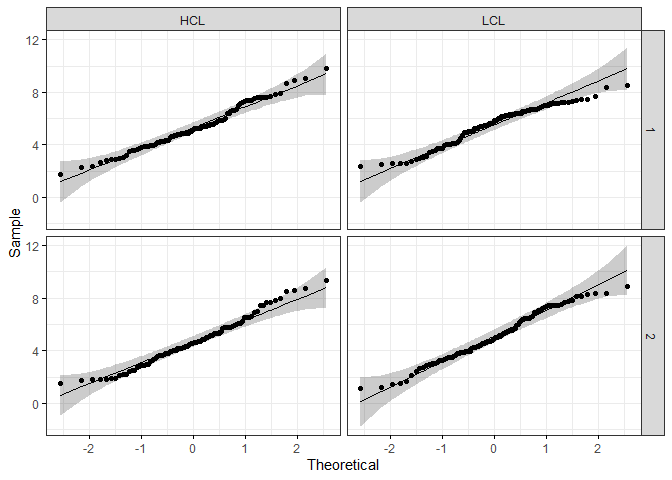
\includegraphics{ALL_TOGETHER_files/figure-latex/VASf-3}

\begin{Shaded}
\begin{Highlighting}[]
\FunctionTok{ggqqplot}\NormalTok{(VAS, }\StringTok{"Mean"}\NormalTok{, }\AttributeTok{ggtheme =} \FunctionTok{theme\_bw}\NormalTok{()) }\SpecialCharTok{+}
  \FunctionTok{facet\_grid}\NormalTok{( }\SpecialCharTok{\textasciitilde{}}\NormalTok{Condition) }\CommentTok{\#  very obviously NOT a normal distribution}
\end{Highlighting}
\end{Shaded}

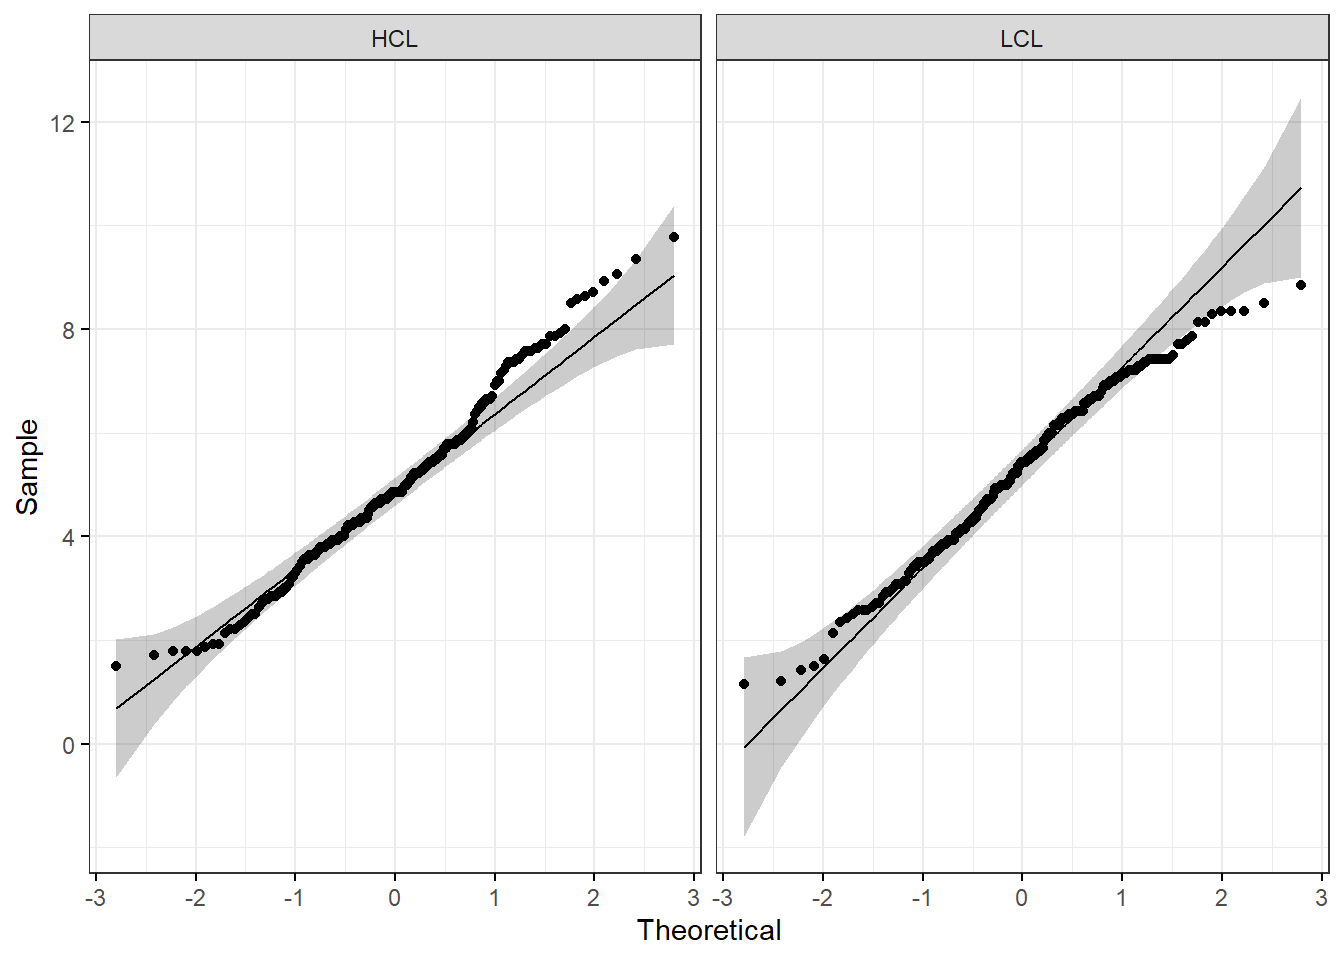
\includegraphics{ALL_TOGETHER_files/figure-latex/VASf-4}

\begin{Shaded}
\begin{Highlighting}[]
\CommentTok{\# SPHERICITY: Mauchly\textquotesingle{}s test}
\NormalTok{x}\OtherTok{\textless{}{-}}\FunctionTok{anova\_test}\NormalTok{(}\AttributeTok{data=}\NormalTok{ VAS, }\AttributeTok{dv=}\NormalTok{ Mean, }\AttributeTok{wid=}\NormalTok{ ID, }\AttributeTok{between=}\NormalTok{ Condition, }\AttributeTok{within=} \FunctionTok{c}\NormalTok{(Time, Day))}
\FunctionTok{get\_anova\_table}\NormalTok{(x, }\AttributeTok{correction =} \FunctionTok{c}\NormalTok{(}\StringTok{\textquotesingle{}GG\textquotesingle{}}\NormalTok{)) }\CommentTok{\#variances are NOT equal! }
\end{Highlighting}
\end{Shaded}

\begin{verbatim}
## ANOVA Table (type III tests)
## 
##               Effect DFn DFd      F        p p<.05      ges
## 1          Condition   1  95  1.152 2.86e-01       9.00e-03
## 2               Time   1  95 26.486 1.43e-06     * 1.30e-02
## 3                Day   1  95 10.908 1.00e-03     * 2.40e-02
## 4     Condition:Time   1  95  0.064 8.01e-01       3.12e-05
## 5      Condition:Day   1  95  0.206 6.51e-01       4.61e-04
## 6           Time:Day   1  95  0.122 7.28e-01       2.86e-05
## 7 Condition:Time:Day   1  95  0.094 7.60e-01       2.20e-05
\end{verbatim}

\begin{Shaded}
\begin{Highlighting}[]
\NormalTok{x}\SpecialCharTok{$}\StringTok{\textquotesingle{}Sphericity Corrections\textquotesingle{}}
\end{Highlighting}
\end{Shaded}

\begin{verbatim}
## NULL
\end{verbatim}

\begin{Shaded}
\begin{Highlighting}[]
\CommentTok{\# OUTLIERS}
\FunctionTok{summary}\NormalTok{(VAS}\SpecialCharTok{$}\NormalTok{Mean)}
\end{Highlighting}
\end{Shaded}

\begin{verbatim}
##    Min. 1st Qu.  Median    Mean 3rd Qu.    Max. 
##   1.143   3.929   5.071   5.148   6.429   9.786
\end{verbatim}

\begin{Shaded}
\begin{Highlighting}[]
\NormalTok{outliers }\OtherTok{\textless{}{-}} \FunctionTok{boxplot}\NormalTok{(VAS}\SpecialCharTok{$}\NormalTok{Mean, }\AttributeTok{plot=}\ConstantTok{FALSE}\NormalTok{)}\SpecialCharTok{$}\NormalTok{out}
\CommentTok{\#visualise}
\NormalTok{d}\OtherTok{\textless{}{-}}\FunctionTok{melt}\NormalTok{(}\FunctionTok{data.frame}\NormalTok{(}\AttributeTok{VAS=}\FunctionTok{c}\NormalTok{(VAS}\SpecialCharTok{$}\NormalTok{Mean))) }\CommentTok{\# we melt to wide format}
\FunctionTok{distribution\_plot}\NormalTok{ (d, }\StringTok{\textquotesingle{}Mean\textquotesingle{}}\NormalTok{)}
\end{Highlighting}
\end{Shaded}

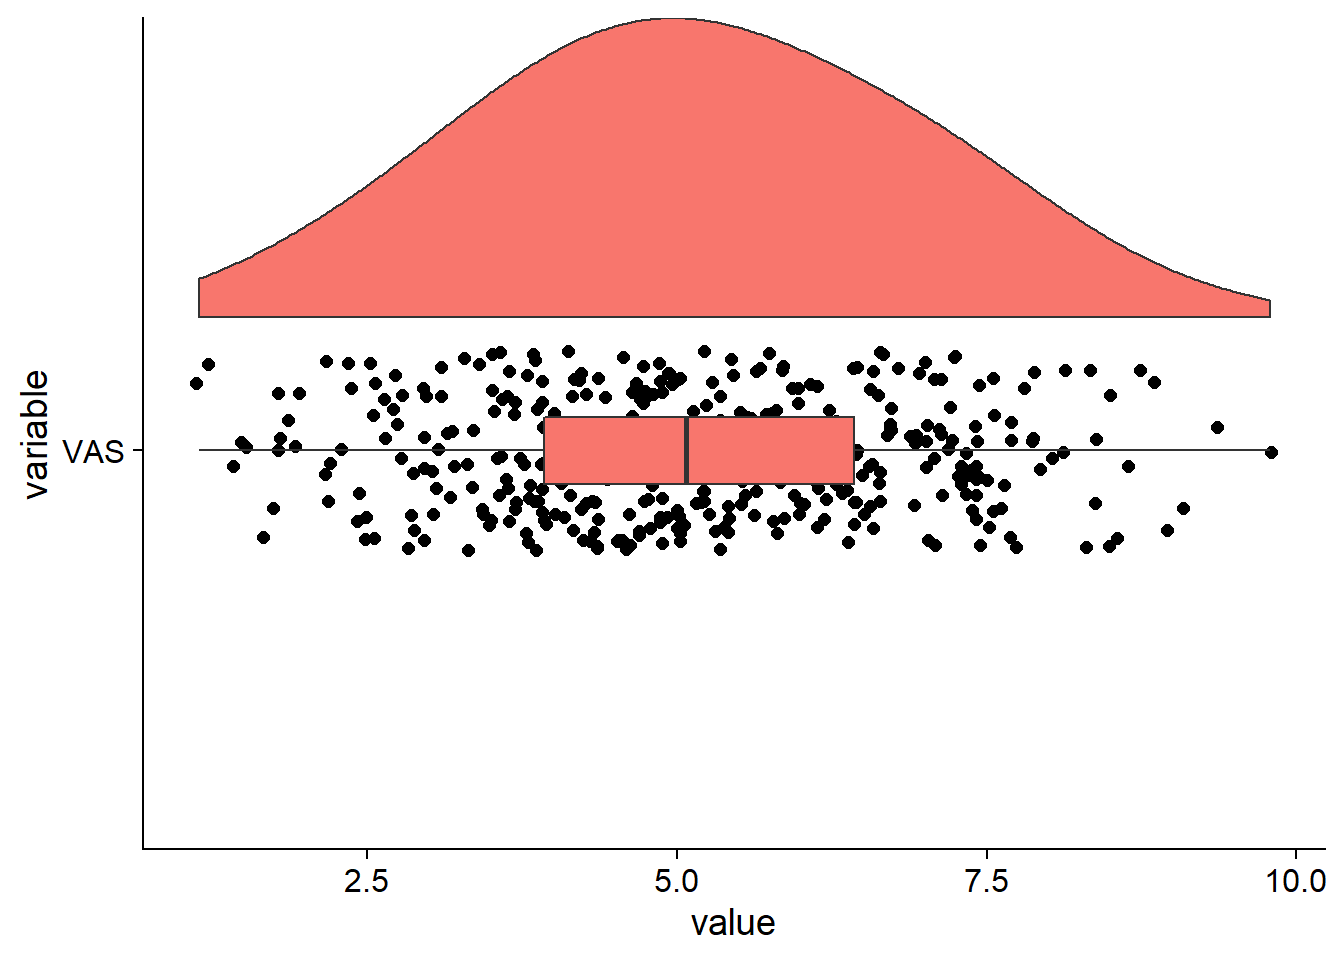
\includegraphics{ALL_TOGETHER_files/figure-latex/VASf-5}

\begin{Shaded}
\begin{Highlighting}[]
\FunctionTok{qqPlot}\NormalTok{(VAS}\SpecialCharTok{$}\NormalTok{Mean) }
\end{Highlighting}
\end{Shaded}

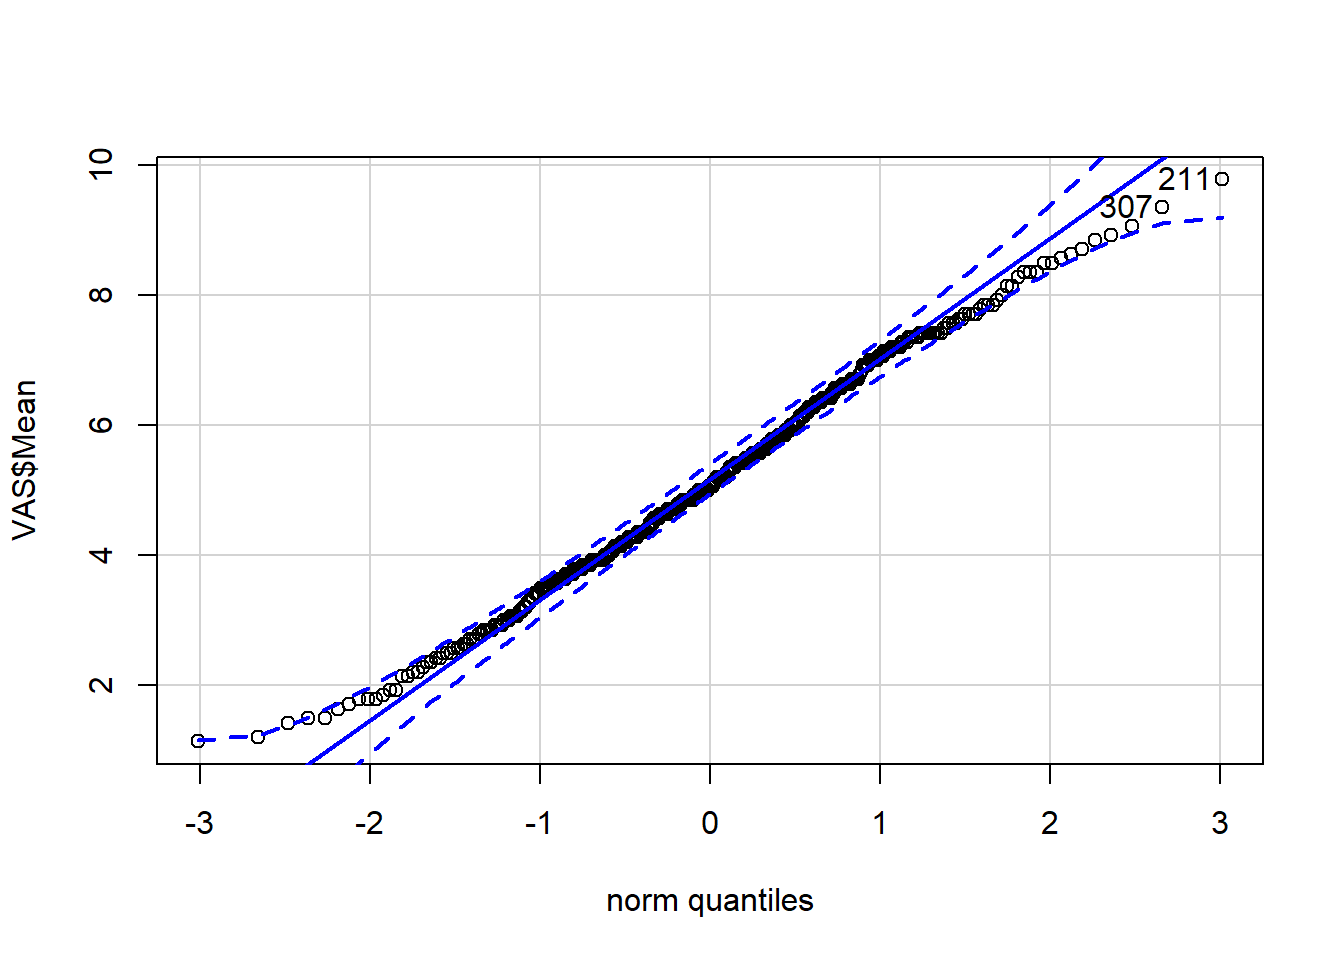
\includegraphics{ALL_TOGETHER_files/figure-latex/VASf-6}

\begin{verbatim}
## [1] 213 310
\end{verbatim}

\begin{Shaded}
\begin{Highlighting}[]
\DocumentationTok{\#\#\#\# repeated{-}measures ANOVA \#\#\#\#}
\FunctionTok{get\_anova\_table}\NormalTok{(x)}
\end{Highlighting}
\end{Shaded}

\begin{verbatim}
## ANOVA Table (type III tests)
## 
##               Effect DFn DFd      F        p p<.05      ges
## 1          Condition   1  95  1.152 2.86e-01       9.00e-03
## 2               Time   1  95 26.486 1.43e-06     * 1.30e-02
## 3                Day   1  95 10.908 1.00e-03     * 2.40e-02
## 4     Condition:Time   1  95  0.064 8.01e-01       3.12e-05
## 5      Condition:Day   1  95  0.206 6.51e-01       4.61e-04
## 6           Time:Day   1  95  0.122 7.28e-01       2.86e-05
## 7 Condition:Time:Day   1  95  0.094 7.60e-01       2.20e-05
\end{verbatim}

\begin{Shaded}
\begin{Highlighting}[]
\CommentTok{\#tukey\textquotesingle{}s post{-}hoc analyses: see if performance decreased faster in HCL compared to LCL}
\NormalTok{two\_w }\OtherTok{\textless{}{-}} \FunctionTok{lm}\NormalTok{(Mean }\SpecialCharTok{\textasciitilde{}}\NormalTok{ Time}\SpecialCharTok{*}\NormalTok{Condition, }\AttributeTok{data=}\NormalTok{ VAS)}
\NormalTok{exp.av }\OtherTok{\textless{}{-}} \FunctionTok{aov}\NormalTok{(two\_w)}
\FunctionTok{summary}\NormalTok{(exp.av)}
\end{Highlighting}
\end{Shaded}

\begin{verbatim}
##                 Df Sum Sq Mean Sq F value Pr(>F)  
## Time             1   14.0  13.950   4.843 0.0283 *
## Condition        1    9.4   9.406   3.266 0.0715 .
## Time:Condition   1    0.0   0.034   0.012 0.9139  
## Residuals      384 1106.0   2.880                 
## ---
## Signif. codes:  0 '***' 0.001 '**' 0.01 '*' 0.05 '.' 0.1 ' ' 1
\end{verbatim}

\begin{Shaded}
\begin{Highlighting}[]
\NormalTok{tukey.test }\OtherTok{\textless{}{-}} \FunctionTok{TukeyHSD}\NormalTok{(exp.av)}
\NormalTok{tukey.test}\SpecialCharTok{$}\NormalTok{Time }
\end{Highlighting}
\end{Shaded}

\begin{verbatim}
##          diff        lwr       upr      p adj
## 2-1 0.3792342 0.04042692 0.7180414 0.02834725
\end{verbatim}

\begin{Shaded}
\begin{Highlighting}[]
\NormalTok{emmeans1}\OtherTok{\textless{}{-}} \FunctionTok{emmeans}\NormalTok{(two\_w, pairwise }\SpecialCharTok{\textasciitilde{}}\NormalTok{ Time}\SpecialCharTok{*}\NormalTok{Condition, }\AttributeTok{adjust =}\StringTok{"fdr"}\NormalTok{, }\AttributeTok{type =} \StringTok{"response"}\NormalTok{)}
\NormalTok{emmean\_dataframe1 }\OtherTok{\textless{}{-}} \FunctionTok{summary}\NormalTok{(emmeans1)}\SpecialCharTok{$}\NormalTok{emmeans}
\FunctionTok{Anova}\NormalTok{(two\_w, }\AttributeTok{type=}\StringTok{\textquotesingle{}III\textquotesingle{}}\NormalTok{)}
\end{Highlighting}
\end{Shaded}

\begin{verbatim}
## Anova Table (Type III tests)
## 
## Response: Mean
##                 Sum Sq  Df  F value Pr(>F)    
## (Intercept)    2204.17   1 765.2537 <2e-16 ***
## Time              7.61   1   2.6407 0.1050    
## Condition         5.28   1   1.8341 0.1764    
## Time:Condition    0.03   1   0.0117 0.9139    
## Residuals      1106.04 384                    
## ---
## Signif. codes:  0 '***' 0.001 '**' 0.01 '*' 0.05 '.' 0.1 ' ' 1
\end{verbatim}

\begin{Shaded}
\begin{Highlighting}[]
\FunctionTok{summary}\NormalTok{(emmeans1)}
\end{Highlighting}
\end{Shaded}

\begin{verbatim}
## $emmeans
##  Time Condition emmean    SE  df lower.CL upper.CL
##  1    HCL         4.79 0.173 384     4.45     5.13
##  2    HCL         5.19 0.173 384     4.85     5.53
##  1    LCL         5.12 0.171 384     4.78     5.46
##  2    LCL         5.48 0.171 384     5.15     5.82
## 
## Confidence level used: 0.95 
## 
## $contrasts
##  contrast      estimate    SE  df t.ratio p.value
##  1 HCL - 2 HCL   -0.398 0.245 384  -1.625  0.2647
##  1 HCL - 1 LCL   -0.330 0.244 384  -1.354  0.2647
##  1 HCL - 2 LCL   -0.691 0.244 384  -2.835  0.0290
##  2 HCL - 1 LCL    0.068 0.244 384   0.279  0.7803
##  2 HCL - 2 LCL   -0.293 0.244 384  -1.201  0.2764
##  1 LCL - 2 LCL   -0.361 0.242 384  -1.488  0.2647
## 
## P value adjustment: fdr method for 6 tests
\end{verbatim}

\begin{Shaded}
\begin{Highlighting}[]
\NormalTok{three\_w }\OtherTok{\textless{}{-}} \FunctionTok{lm}\NormalTok{(Mean }\SpecialCharTok{\textasciitilde{}}\NormalTok{ Time}\SpecialCharTok{*}\NormalTok{Condition}\SpecialCharTok{*}\NormalTok{Day, }\AttributeTok{data=}\NormalTok{ VAS)}
\NormalTok{exp.av }\OtherTok{\textless{}{-}} \FunctionTok{aov}\NormalTok{(three\_w)}
\FunctionTok{summary}\NormalTok{(exp.av)}
\end{Highlighting}
\end{Shaded}

\begin{verbatim}
##                     Df Sum Sq Mean Sq F value  Pr(>F)   
## Time                 1   14.0  13.950   4.912 0.02726 * 
## Condition            1    9.4   9.406   3.312 0.06956 . 
## Day                  1   26.3  26.291   9.258 0.00251 **
## Time:Condition       1    0.0   0.034   0.012 0.91332   
## Time:Day             1    0.0   0.030   0.011 0.91779   
## Condition:Day        1    0.5   0.498   0.175 0.67566   
## Time:Condition:Day   1    0.0   0.024   0.008 0.92719   
## Residuals          380 1079.2   2.840                   
## ---
## Signif. codes:  0 '***' 0.001 '**' 0.01 '*' 0.05 '.' 0.1 ' ' 1
\end{verbatim}

\begin{Shaded}
\begin{Highlighting}[]
\NormalTok{tukey.test }\OtherTok{\textless{}{-}} \FunctionTok{TukeyHSD}\NormalTok{(exp.av)}
\NormalTok{tukey.test}\SpecialCharTok{$}\NormalTok{Time }\CommentTok{\#t1 \textgreater{} t4 \& t5, t2 \textgreater{}t4 \& t5!}
\end{Highlighting}
\end{Shaded}

\begin{verbatim}
##          diff        lwr       upr      p adj
## 2-1 0.3792342 0.04279553 0.7156728 0.02726035
\end{verbatim}

\begin{Shaded}
\begin{Highlighting}[]
\NormalTok{emmeans1}\OtherTok{\textless{}{-}} \FunctionTok{emmeans}\NormalTok{(three\_w, pairwise }\SpecialCharTok{\textasciitilde{}}\NormalTok{ Time}\SpecialCharTok{*}\NormalTok{Condition}\SpecialCharTok{*}\NormalTok{Day, }\AttributeTok{adjust =}\StringTok{"fdr"}\NormalTok{, }\AttributeTok{type =} \StringTok{"response"}\NormalTok{)}
\NormalTok{emmean\_dataframe }\OtherTok{\textless{}{-}} \FunctionTok{summary}\NormalTok{(emmeans1)}\SpecialCharTok{$}\NormalTok{emmeans}
\FunctionTok{Anova}\NormalTok{(three\_w, }\AttributeTok{type=}\StringTok{\textquotesingle{}III\textquotesingle{}}\NormalTok{)}
\end{Highlighting}
\end{Shaded}

\begin{verbatim}
## Anova Table (Type III tests)
## 
## Response: Mean
##                     Sum Sq  Df  F value Pr(>F)    
## (Intercept)        1234.53   1 434.6958 <2e-16 ***
## Time                  4.47   1   1.5738 0.2104    
## Condition             1.82   1   0.6412 0.4238    
## Day                   7.51   1   2.6456 0.1047    
## Time:Condition        0.06   1   0.0201 0.8874    
## Time:Day              0.05   1   0.0189 0.8906    
## Condition:Day         0.15   1   0.0536 0.8171    
## Time:Condition:Day    0.02   1   0.0084 0.9272    
## Residuals          1079.20 380                    
## ---
## Signif. codes:  0 '***' 0.001 '**' 0.01 '*' 0.05 '.' 0.1 ' ' 1
\end{verbatim}

\begin{Shaded}
\begin{Highlighting}[]
\FunctionTok{summary}\NormalTok{(emmeans1)}
\end{Highlighting}
\end{Shaded}

\begin{verbatim}
## $emmeans
##  Time Condition Day emmean    SE  df lower.CL upper.CL
##  1    HCL       1     5.07 0.243 380     4.59     5.55
##  2    HCL       1     5.50 0.243 380     5.02     5.98
##  1    LCL       1     5.35 0.241 380     4.87     5.82
##  2    LCL       1     5.71 0.241 380     5.24     6.18
##  1    HCL       2     4.51 0.243 380     4.03     4.99
##  2    HCL       2     4.88 0.243 380     4.40     5.35
##  1    LCL       2     4.90 0.241 380     4.42     5.37
##  2    LCL       2     5.26 0.241 380     4.78     5.73
## 
## Confidence level used: 0.95 
## 
## $contrasts
##  contrast          estimate    SE  df t.ratio p.value
##  1 HCL 1 - 2 HCL 1  -0.4315 0.344 380  -1.255  0.4209
##  1 HCL 1 - 1 LCL 1  -0.2741 0.342 380  -0.801  0.5933
##  1 HCL 1 - 2 LCL 1  -0.6370 0.342 380  -1.861  0.2423
##  1 HCL 1 - 1 HCL 2   0.5595 0.344 380   1.627  0.2931
##  1 HCL 1 - 2 HCL 2   0.1949 0.344 380   0.567  0.6860
##  1 HCL 1 - 1 LCL 2   0.1735 0.342 380   0.507  0.6860
##  1 HCL 1 - 2 LCL 2  -0.1851 0.342 380  -0.541  0.6860
##  2 HCL 1 - 1 LCL 1   0.1575 0.342 380   0.460  0.6953
##  2 HCL 1 - 2 LCL 1  -0.2055 0.342 380  -0.600  0.6860
##  2 HCL 1 - 1 HCL 2   0.9911 0.344 380   2.881  0.0586
##  2 HCL 1 - 2 HCL 2   0.6265 0.344 380   1.821  0.2423
##  2 HCL 1 - 1 LCL 2   0.6050 0.342 380   1.768  0.2423
##  2 HCL 1 - 2 LCL 2   0.2464 0.342 380   0.720  0.6293
##  1 LCL 1 - 2 LCL 1  -0.3630 0.340 380  -1.066  0.4316
##  1 LCL 1 - 1 HCL 2   0.8336 0.342 380   2.436  0.0996
##  1 LCL 1 - 2 HCL 2   0.4690 0.342 380   1.370  0.4081
##  1 LCL 1 - 1 LCL 2   0.4475 0.340 380   1.314  0.4081
##  1 LCL 1 - 2 LCL 2   0.0889 0.340 380   0.261  0.8235
##  2 LCL 1 - 1 HCL 2   1.1966 0.342 380   3.496  0.0148
##  2 LCL 1 - 2 HCL 2   0.8320 0.342 380   2.431  0.0996
##  2 LCL 1 - 1 LCL 2   0.8105 0.340 380   2.381  0.0996
##  2 LCL 1 - 2 LCL 2   0.4519 0.340 380   1.327  0.4081
##  1 HCL 2 - 2 HCL 2  -0.3646 0.344 380  -1.060  0.4316
##  1 HCL 2 - 1 LCL 2  -0.3861 0.342 380  -1.128  0.4316
##  1 HCL 2 - 2 LCL 2  -0.7447 0.342 380  -2.176  0.1408
##  2 HCL 2 - 1 LCL 2  -0.0215 0.342 380  -0.063  0.9500
##  2 HCL 2 - 2 LCL 2  -0.3801 0.342 380  -1.111  0.4316
##  1 LCL 2 - 2 LCL 2  -0.3586 0.340 380  -1.053  0.4316
## 
## P value adjustment: fdr method for 28 tests
\end{verbatim}

\begin{Shaded}
\begin{Highlighting}[]
\CommentTok{\#summary }
\NormalTok{sum }\OtherTok{\textless{}{-}} \FunctionTok{sum\_3}\NormalTok{ (VAS, }\StringTok{\textquotesingle{}Time\textquotesingle{}}\NormalTok{, }\StringTok{\textquotesingle{}Condition\textquotesingle{}}\NormalTok{, }\StringTok{\textquotesingle{}Day\textquotesingle{}}\NormalTok{, }\StringTok{\textquotesingle{}Mean\textquotesingle{}}\NormalTok{)}
\NormalTok{sum}
\end{Highlighting}
\end{Shaded}

\begin{verbatim}
## # A tibble: 8 x 8
## # Groups:   Time, Condition [4]
##   Time  Condition Day       n  mean    sd    se    ic
##   <fct> <fct>     <fct> <int> <dbl> <dbl> <dbl> <dbl>
## 1 1     HCL       1        48  5.07  1.43 0.207 0.417
## 2 1     HCL       2        48  4.51  1.60 0.231 0.465
## 3 1     LCL       1        49  5.35  1.38 0.197 0.396
## 4 1     LCL       2        49  4.90  1.70 0.243 0.488
## 5 2     HCL       1        48  5.50  1.81 0.261 0.526
## 6 2     HCL       2        48  4.88  1.93 0.279 0.562
## 7 2     LCL       1        49  5.71  1.55 0.221 0.444
## 8 2     LCL       2        49  5.26  1.98 0.282 0.568
\end{verbatim}

\begin{Shaded}
\begin{Highlighting}[]
\DocumentationTok{\#\# VISUALISATION}
\CommentTok{\# boxplot }
\NormalTok{bxp }\OtherTok{\textless{}{-}} \FunctionTok{ggboxplot}\NormalTok{(}
\NormalTok{  VAS, }\AttributeTok{x =} \StringTok{"Condition"}\NormalTok{, }\AttributeTok{y =} \StringTok{"Mean"}\NormalTok{,}
  \AttributeTok{color =} \StringTok{"Time"}\NormalTok{, }\AttributeTok{palette =} \StringTok{"jco"}\NormalTok{,}
  \AttributeTok{facet.by =} \StringTok{"Day"}\NormalTok{, }\AttributeTok{short.panel.labs =} \ConstantTok{FALSE}
\NormalTok{  )}
\NormalTok{bxp}
\end{Highlighting}
\end{Shaded}

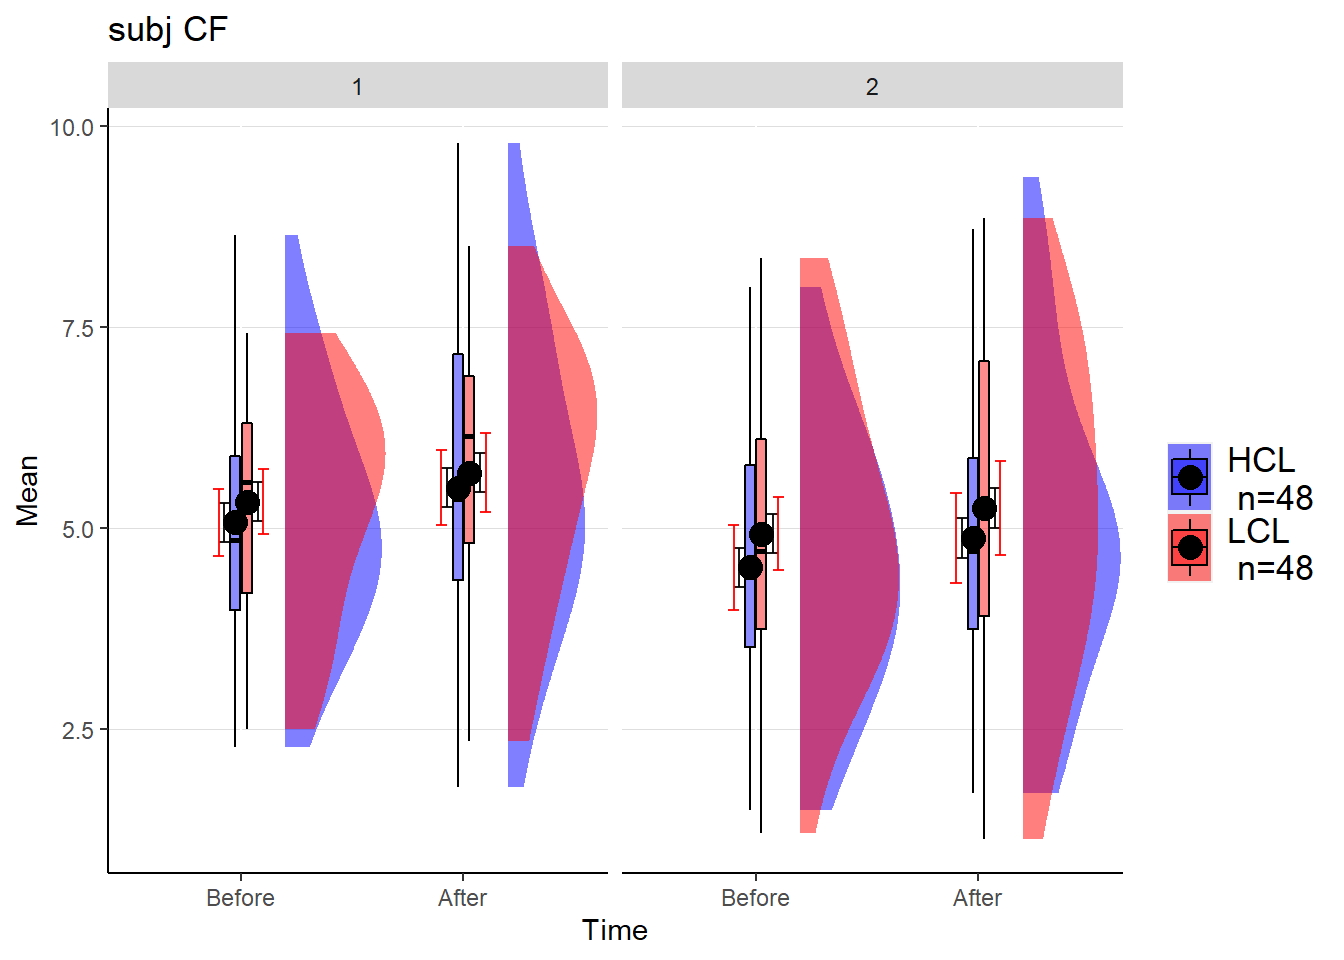
\includegraphics{ALL_TOGETHER_files/figure-latex/VASf-7}

\begin{Shaded}
\begin{Highlighting}[]
\DocumentationTok{\#\# plot with error bars}
\NormalTok{pl }\OtherTok{\textless{}{-}} \FunctionTok{plotty}\NormalTok{(VAS, emmean\_dataframe, }\StringTok{\textquotesingle{}Time\textquotesingle{}}\NormalTok{, }\StringTok{\textquotesingle{}Mean\textquotesingle{}}\NormalTok{, }\StringTok{\textquotesingle{}Condition\textquotesingle{}}\NormalTok{, }\StringTok{\textquotesingle{}emmean\textquotesingle{}}\NormalTok{, }\StringTok{\textquotesingle{}subj CF\textquotesingle{}}\NormalTok{) }\SpecialCharTok{+}
 \FunctionTok{facet\_grid}\NormalTok{(.}\SpecialCharTok{\textasciitilde{}}\NormalTok{Day)}\SpecialCharTok{+}
\FunctionTok{scale\_x\_discrete}\NormalTok{(}\AttributeTok{labels=}\FunctionTok{c}\NormalTok{(}\StringTok{"Before"}\NormalTok{, }\StringTok{"After"}\NormalTok{))}
\FunctionTok{ggsave}\NormalTok{(pl, }\AttributeTok{file=}\FunctionTok{paste0}\NormalTok{(plotPrefix, }\StringTok{"VAS\_Plot.jpg"}\NormalTok{), }\AttributeTok{width =} \DecValTok{2500}\NormalTok{, }\AttributeTok{height =} \DecValTok{1500}\NormalTok{, }\AttributeTok{dpi =} \DecValTok{300}\NormalTok{, }\AttributeTok{units =} \StringTok{"px"}\NormalTok{)}
\NormalTok{pl}
\end{Highlighting}
\end{Shaded}

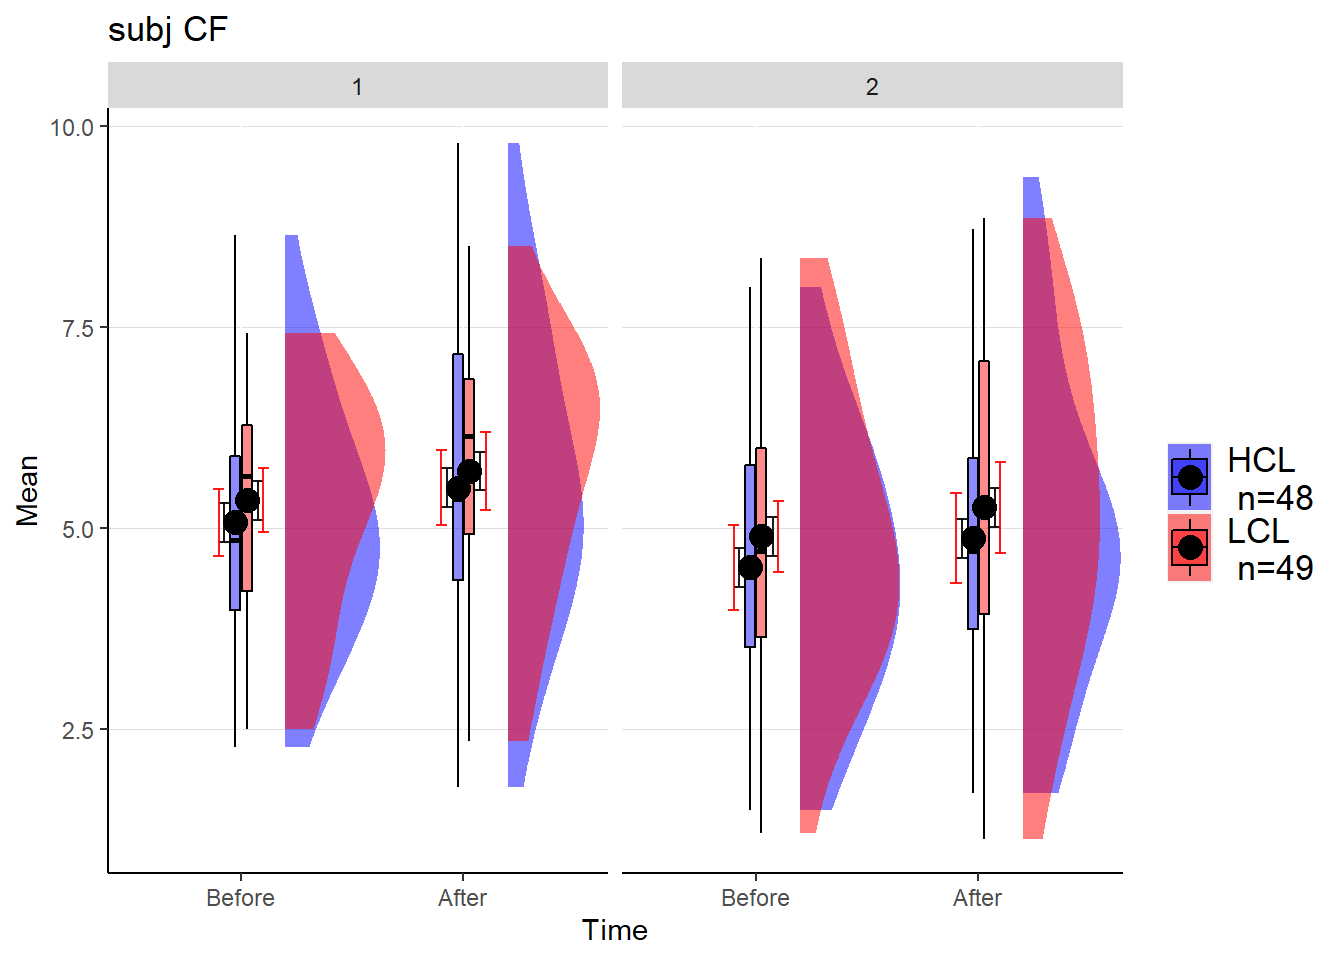
\includegraphics{ALL_TOGETHER_files/figure-latex/VASf-8}

\begin{Shaded}
\begin{Highlighting}[]
\CommentTok{\# }
\CommentTok{\# \# difference score, devide by baseline (pre TloadBack) as a function of group (Day/condition): (2{-}1)/1}
\CommentTok{\# for (i in 1:97) \{}
\CommentTok{\#   VAS$Diff[VAS$ID==i \& VAS$Day==1] = }
\CommentTok{\#     ((VAS$Mean[VAS$Test==2 \& VAS$ID==i \& VAS$Day==1]{-} VAS$Mean[VAS$Test==1 \& VAS$ID==i \& VAS$Day==1])/VAS$Mean[VAS$Test==1 \& VAS$ID==i \& VAS$Day==1])}
\CommentTok{\#   VAS$Diff[VAS$ID==i \& VAS$Day==2] = }
\CommentTok{\#     ((VAS$Mean[VAS$Test==2 \& VAS$ID==i \& VAS$Day==1]{-} VAS$Mean[VAS$Test==1 \& VAS$ID==i \& VAS$Day==2])/VAS$Mean[VAS$Test==1 \& VAS$ID==i \& VAS$Day==2])}
\CommentTok{\# \}}
\CommentTok{\# }\AlertTok{\#\#\#}\CommentTok{ CHECKING ASSUMPTIONS \#\#\#\#}
\CommentTok{\# \# Time x Condition 2{-}way ANOVA with interaction effect (what Borrogan did)}
\CommentTok{\# res.aov2 \textless{}{-} aov(Diff \textasciitilde{} Condition * Day, data= VAS)}
\CommentTok{\# summary(res.aov2)}
\CommentTok{\# \# HOMOGENEITY OF VARIANCE}
\CommentTok{\# plot(res.aov2, 1) \# residuqls vs fits plot shows no evident relationship residuals and fitted values (Diffs of groups)}
\CommentTok{\# }
\CommentTok{\# \# NORMALITY}
\CommentTok{\# aov\_residuals \textless{}{-} residuals (object=res.aov2)}
\CommentTok{\# shapiro.test(x=aov\_residuals) \#  }
\CommentTok{\# VAS \%\textgreater{}\%}
\CommentTok{\#   group\_by(Condition, Day) \%\textgreater{}\%}
\CommentTok{\#   shapiro\_test(Diff) \# }
\CommentTok{\# \#visualisation}
\CommentTok{\# plot(res.aov2, 2) \#normal}
\CommentTok{\# ggqqplot(VAS, "Diff", ggtheme = theme\_bw()) +}
\CommentTok{\#   facet\_grid(Day \textasciitilde{} Condition)}
\CommentTok{\# ggqqplot(VAS, "Diff", ggtheme = theme\_bw()) +}
\CommentTok{\#   facet\_grid( \textasciitilde{}Condition) \#  very obviously NOT a normal distribution}
\CommentTok{\# }
\CommentTok{\# \# SPHERICITY: Mauchly\textquotesingle{}s test}
\CommentTok{\# x\textless{}{-}anova\_test(data= VAS, dv= Diff, wid= ID, between= Condition, within= c(Time, Day))}
\CommentTok{\# get\_anova\_table(x, correction = c(\textquotesingle{}GG\textquotesingle{})) \#variances are NOT equal! }
\CommentTok{\# x$\textquotesingle{}Sphericity Corrections\textquotesingle{}}
\CommentTok{\# }
\CommentTok{\# \# OUTLIERS}
\CommentTok{\# summary(VAS$Diff)}
\CommentTok{\# outliers \textless{}{-} boxplot(VAS$Diff, plot=FALSE)$out}
\CommentTok{\# \# remove }
\CommentTok{\#  VAS\textless{}{-} VAS[{-}which(VAS$Diff \%in\% outliers),]}
\CommentTok{\# \#visualise}
\CommentTok{\# d\textless{}{-}melt(data.frame(VAS=c(VAS$Diff))) \# we melt to wide format}
\CommentTok{\# distribution\_plot (d, \textquotesingle{}Diff\textquotesingle{})}
\CommentTok{\# qqPlot(VAS$Diff) }
\CommentTok{\# }
\CommentTok{\# }
\CommentTok{\# \#\#\#\# repeated{-}measures ANOVA \#\#\#\#}
\CommentTok{\# x\textless{}{-}anova\_test(data= VAS, dv= Diff, wid= ID, between= Condition, within= c(Time, Day))}
\CommentTok{\# get\_anova\_table(x)}
\CommentTok{\# }
\CommentTok{\# \#tukey\textquotesingle{}s post{-}hoc analyses: see if performance decreased faster in HCL compared to LCL}
\CommentTok{\# two\_w \textless{}{-} lm(Diff \textasciitilde{} Time*Condition, data= VAS)}
\CommentTok{\# exp.av \textless{}{-} aov(two\_w)}
\CommentTok{\# summary(exp.av)}
\CommentTok{\# tukey.test \textless{}{-} TukeyHSD(exp.av)}
\CommentTok{\# tukey.test$Time }
\CommentTok{\# emmeans1\textless{}{-} emmeans(two\_w, pairwise \textasciitilde{} Time*Condition, adjust ="fdr", type = "response")}
\CommentTok{\# emDiff\_dataframe \textless{}{-} summary(emmeans1)$emmeans}
\CommentTok{\# Anova(two\_w, type=\textquotesingle{}III\textquotesingle{})}
\CommentTok{\# summary(emmeans1)}
\CommentTok{\# }
\CommentTok{\# \#summary }
\CommentTok{\# sum \textless{}{-} sum\_3 (VAS, \textquotesingle{}Time\textquotesingle{}, \textquotesingle{}Condition\textquotesingle{}, \textquotesingle{}Day\textquotesingle{}, \textquotesingle{}Diff\textquotesingle{})}
\CommentTok{\# sum}
\CommentTok{\# }
\CommentTok{\# \#\# VISUALISATION}
\CommentTok{\# \# boxplot }
\CommentTok{\# bxp \textless{}{-} ggboxplot(}
\CommentTok{\#   VAS, x = "Condition", y = "Diff",}
\CommentTok{\#   color = "Time", palette = "jco",}
\CommentTok{\#   facet.by = "Day", short.panel.labs = FALSE}
\CommentTok{\#   )}
\CommentTok{\# \#\# plot with error bars}
\CommentTok{\# pl \textless{}{-} plotty(VAS, emmean\_dataframe, \textquotesingle{}Day\textquotesingle{}, \textquotesingle{}Diff\textquotesingle{}, \textquotesingle{}Condition\textquotesingle{}, \textquotesingle{}emmean\textquotesingle{}, \textquotesingle{}subj CF\textquotesingle{})}
\CommentTok{\# scale\_x\_discrete(labels=c("Before", "After"))}
\end{Highlighting}
\end{Shaded}

\begin{center}\rule{0.5\linewidth}{0.5pt}\end{center}

\hypertarget{objective-cf}{%
\subsection{Objective CF}\label{objective-cf}}

\begin{itemize}
\tightlist
\item
  We will test the evolution of Performance (weighted accuracy) during
  TloadDback with Condition (HCL/LCL) and Time (t1-t3) as within-subject
  factors.
\item
  interested in main effect e.g.~t1\textgreater t4 and Condition x Time
  interaction on the Acc
\end{itemize}

\begin{Shaded}
\begin{Highlighting}[]
\DocumentationTok{\#\#\#\#\#\#\#\#\#\#\#\#\#\#\#\#\#\#\#\#\#\#\#\#\#\#\#\#\#\#\#\#\#\#\#\#\#\#\#\#\#\#}
  \DocumentationTok{\#\#\# PERFORMANCE/ ACCURACY/ OBJECTIVE CF }\AlertTok{\#\#\#}
\DocumentationTok{\#\#\#\#\#\#\#\#\#\#\#\#\#\#\#\#\#\#\#\#\#\#\#\#\#\#\#\#\#\#\#\#\#\#\#\#\#\#\#\#\#}

\DocumentationTok{\#\#\#\# DOWNLOAD + CLEAN DATA \#\#\#\#}
\NormalTok{data}\OtherTok{\textless{}{-}} \FunctionTok{read.csv}\NormalTok{(}\FunctionTok{paste0}\NormalTok{(Dir, }\StringTok{"EXP.csv"}\NormalTok{), }\AttributeTok{header =} \ConstantTok{TRUE}\NormalTok{, }\AttributeTok{sep =}\NormalTok{ )}
\CommentTok{\# we remove rows that have prop\_correct == NA , because these are lines in the data where the ERROR message was shown (accuracy=0)}
\NormalTok{data }\OtherTok{\textless{}{-}}\NormalTok{ data[}\SpecialCharTok{!}\FunctionTok{is.na}\NormalTok{(data}\SpecialCharTok{$}\NormalTok{prop\_correct),]}
\CommentTok{\# create a trial.index that goes from 1 to the number of trials:  not every participant has equal amount of trials, depends on their speed/accuracy}
\ControlFlowTok{for}\NormalTok{ (i }\ControlFlowTok{in} \DecValTok{1}\SpecialCharTok{:}\DecValTok{97}\NormalTok{) \{ data}\SpecialCharTok{$}\NormalTok{trial.index[data}\SpecialCharTok{$}\NormalTok{ID}\SpecialCharTok{==}\NormalTok{i]}\OtherTok{=} \DecValTok{1}\SpecialCharTok{:}\FunctionTok{length}\NormalTok{(}\FunctionTok{unique}\NormalTok{(data}\SpecialCharTok{$}\NormalTok{Trial.Index[data}\SpecialCharTok{$}\NormalTok{ID }\SpecialCharTok{==}\NormalTok{i]))\}}

\CommentTok{\# length(data$trial.index[is.na(data$trial.index)]) }
\CommentTok{\# data = subset(data, select = {-}c(Local.Date, Participant.Private.ID, Task.Name, Accuracy\_Level, Time.Elapsed, Trial.Index))}

\CommentTok{\# create var Time that indicates if it is part of t1, t2, t3. t1 is the first 40\%, t2 middle 20\%, t3 last 40\% }
\CommentTok{\# we work with percentages because the \#trials differs per ptt AND per day: }
\ControlFlowTok{for}\NormalTok{ (i }\ControlFlowTok{in} \DecValTok{1}\SpecialCharTok{:}\DecValTok{97}\NormalTok{) \{}
\NormalTok{  data}\SpecialCharTok{$}\NormalTok{Time[data}\SpecialCharTok{$}\NormalTok{ID }\SpecialCharTok{==}\NormalTok{i }\SpecialCharTok{\&}\NormalTok{ data}\SpecialCharTok{$}\NormalTok{Day}\SpecialCharTok{==}\DecValTok{1}\NormalTok{] }\OtherTok{=} \DecValTok{2} \CommentTok{\# day 1}
\NormalTok{  data}\SpecialCharTok{$}\NormalTok{Time[data}\SpecialCharTok{$}\NormalTok{ID }\SpecialCharTok{==}\NormalTok{i }\SpecialCharTok{\&}\NormalTok{ data}\SpecialCharTok{$}\NormalTok{Day}\SpecialCharTok{==}\DecValTok{1} \SpecialCharTok{\&}\NormalTok{ data}\SpecialCharTok{$}\NormalTok{trial.index}\SpecialCharTok{\textless{}}\NormalTok{(}\FloatTok{0.6}\SpecialCharTok{*} \FunctionTok{length}\NormalTok{(data}\SpecialCharTok{$}\NormalTok{trial.index[data}\SpecialCharTok{$}\NormalTok{Day}\SpecialCharTok{==}\DecValTok{1} \SpecialCharTok{\&}\NormalTok{ data}\SpecialCharTok{$}\NormalTok{ID}\SpecialCharTok{==}\NormalTok{i])) ] }\OtherTok{=} \StringTok{"middle"}
\NormalTok{  data}\SpecialCharTok{$}\NormalTok{Time[data}\SpecialCharTok{$}\NormalTok{ID }\SpecialCharTok{==}\NormalTok{i }\SpecialCharTok{\&}\NormalTok{ data}\SpecialCharTok{$}\NormalTok{Day}\SpecialCharTok{==}\DecValTok{1} \SpecialCharTok{\&}\NormalTok{ data}\SpecialCharTok{$}\NormalTok{trial.index}\SpecialCharTok{\textless{}}\NormalTok{(}\FloatTok{0.4}\SpecialCharTok{*} \FunctionTok{length}\NormalTok{(data}\SpecialCharTok{$}\NormalTok{trial.index[data}\SpecialCharTok{$}\NormalTok{Day}\SpecialCharTok{==}\DecValTok{1} \SpecialCharTok{\&}\NormalTok{ data}\SpecialCharTok{$}\NormalTok{ID}\SpecialCharTok{==}\NormalTok{i])) ] }\OtherTok{=} \DecValTok{1}
\NormalTok{  data}\SpecialCharTok{$}\NormalTok{Time[data}\SpecialCharTok{$}\NormalTok{ID }\SpecialCharTok{==}\NormalTok{i }\SpecialCharTok{\&}\NormalTok{ data}\SpecialCharTok{$}\NormalTok{Day}\SpecialCharTok{==}\DecValTok{2}\NormalTok{] }\OtherTok{=} \DecValTok{2} \CommentTok{\# day 2}
\NormalTok{  data}\SpecialCharTok{$}\NormalTok{Time[data}\SpecialCharTok{$}\NormalTok{ID }\SpecialCharTok{==}\NormalTok{i }\SpecialCharTok{\&}\NormalTok{ data}\SpecialCharTok{$}\NormalTok{Day}\SpecialCharTok{==}\DecValTok{2} \SpecialCharTok{\&}\NormalTok{ data}\SpecialCharTok{$}\NormalTok{trial.index}\SpecialCharTok{\textless{}}\NormalTok{(}\FloatTok{0.6}\SpecialCharTok{*} \FunctionTok{length}\NormalTok{(data}\SpecialCharTok{$}\NormalTok{trial.index[data}\SpecialCharTok{$}\NormalTok{Day}\SpecialCharTok{==}\DecValTok{2} \SpecialCharTok{\&}\NormalTok{ data}\SpecialCharTok{$}\NormalTok{ID}\SpecialCharTok{==}\NormalTok{i])) ] }\OtherTok{=} \StringTok{"middle"}
\NormalTok{  data}\SpecialCharTok{$}\NormalTok{Time[data}\SpecialCharTok{$}\NormalTok{ID }\SpecialCharTok{==}\NormalTok{i }\SpecialCharTok{\&}\NormalTok{ data}\SpecialCharTok{$}\NormalTok{Day}\SpecialCharTok{==}\DecValTok{2} \SpecialCharTok{\&}\NormalTok{ data}\SpecialCharTok{$}\NormalTok{trial.index}\SpecialCharTok{\textless{}}\NormalTok{(}\FloatTok{0.4}\SpecialCharTok{*} \FunctionTok{length}\NormalTok{(data}\SpecialCharTok{$}\NormalTok{trial.index[data}\SpecialCharTok{$}\NormalTok{Day}\SpecialCharTok{==}\DecValTok{2} \SpecialCharTok{\&}\NormalTok{ data}\SpecialCharTok{$}\NormalTok{ID}\SpecialCharTok{==}\NormalTok{i])) ] }\OtherTok{=} \DecValTok{1}
\NormalTok{\}}
\CommentTok{\#remove \textquotesingle{}middle\textquotesingle{}}
\NormalTok{data }\OtherTok{\textless{}{-}}\NormalTok{ data[}\SpecialCharTok{!}\NormalTok{(data}\SpecialCharTok{$}\NormalTok{Time}\SpecialCharTok{==}\StringTok{"middle"}\NormalTok{),]}
\CommentTok{\# CREATE DATAFRAME, with the Mean prop\_correct per ID, Time, Day, Condition}
\NormalTok{EXP }\OtherTok{\textless{}{-}} \FunctionTok{as.data.frame}\NormalTok{ (}\FunctionTok{group\_by}\NormalTok{(data, Condition, Day, Time, ID) }\SpecialCharTok{\%\textgreater{}\%}
  \FunctionTok{summarise}\NormalTok{(}
    \AttributeTok{count =} \FunctionTok{n}\NormalTok{(),}
    \AttributeTok{Mean =} \FunctionTok{mean}\NormalTok{(prop\_correct, }\AttributeTok{na.rm =} \ConstantTok{TRUE}\NormalTok{)}
\NormalTok{  ))}
\FunctionTok{head}\NormalTok{(EXP) }\CommentTok{\# mean Mean (prop\_correct) per ID, Time, Day and Condition}
\end{Highlighting}
\end{Shaded}

\begin{verbatim}
##   Condition Day Time ID count      Mean
## 1       HCL   1    1 50   179 0.7368638
## 2       HCL   1    1 51   108 0.7615934
## 3       HCL   1    1 52   127 0.6388012
## 4       HCL   1    1 53   102 0.5617524
## 5       HCL   1    1 54    95 0.6043328
## 6       HCL   1    1 55   121 0.6698068
\end{verbatim}

\begin{Shaded}
\begin{Highlighting}[]
\CommentTok{\# set factors}
\NormalTok{EXP}\SpecialCharTok{$}\NormalTok{Time }\OtherTok{\textless{}{-}} \FunctionTok{as.factor}\NormalTok{(EXP}\SpecialCharTok{$}\NormalTok{Time)}
\NormalTok{EXP}\SpecialCharTok{$}\NormalTok{Condition }\OtherTok{\textless{}{-}} \FunctionTok{as.factor}\NormalTok{(EXP}\SpecialCharTok{$}\NormalTok{Condition)}
\NormalTok{EXP}\SpecialCharTok{$}\NormalTok{Day }\OtherTok{\textless{}{-}} \FunctionTok{as.factor}\NormalTok{(EXP}\SpecialCharTok{$}\NormalTok{Day)}
\NormalTok{EXP}\SpecialCharTok{$}\NormalTok{ID }\OtherTok{\textless{}{-}} \FunctionTok{as.factor}\NormalTok{(EXP}\SpecialCharTok{$}\NormalTok{ID)}


\DocumentationTok{\#\#\# CHECKING ASSUMPTIONS \#\#\#\#}

\CommentTok{\# Time x Condition 2{-}way ANOVA with interaction effect}
\NormalTok{res.aov2 }\OtherTok{\textless{}{-}} \FunctionTok{aov}\NormalTok{(Mean }\SpecialCharTok{\textasciitilde{}}\NormalTok{ Condition}\SpecialCharTok{*}\NormalTok{Time, }\AttributeTok{data=}\NormalTok{ EXP)}
\FunctionTok{summary}\NormalTok{(res.aov2)}
\end{Highlighting}
\end{Shaded}

\begin{verbatim}
##                 Df Sum Sq Mean Sq F value   Pr(>F)    
## Condition        1  5.986   5.986  387.32  < 2e-16 ***
## Time             1  0.188   0.188   12.20 0.000534 ***
## Condition:Time   1  0.068   0.068    4.41 0.036380 *  
## Residuals      384  5.935   0.015                     
## ---
## Signif. codes:  0 '***' 0.001 '**' 0.01 '*' 0.05 '.' 0.1 ' ' 1
\end{verbatim}

\begin{Shaded}
\begin{Highlighting}[]
\DocumentationTok{\#\# HOMOGENEITY OF VARIANCE}
\CommentTok{\#Levene\textquotesingle{}s test homogeneity variances}
\FunctionTok{leveneTest}\NormalTok{(Mean}\SpecialCharTok{\textasciitilde{}}\NormalTok{ Time }\SpecialCharTok{*}\NormalTok{ Condition, }\AttributeTok{data=}\NormalTok{ EXP) }\CommentTok{\# no homogeneity! problem! }
\end{Highlighting}
\end{Shaded}

\begin{verbatim}
## Levene's Test for Homogeneity of Variance (center = median)
##        Df F value  Pr(>F)  
## group   3  2.5902 0.05256 .
##       384                  
## ---
## Signif. codes:  0 '***' 0.001 '**' 0.01 '*' 0.05 '.' 0.1 ' ' 1
\end{verbatim}

\begin{Shaded}
\begin{Highlighting}[]
\FunctionTok{box\_m}\NormalTok{(EXP[, }\StringTok{\textquotesingle{}Mean\textquotesingle{}}\NormalTok{, }\AttributeTok{drop=}\ConstantTok{FALSE}\NormalTok{], EXP}\SpecialCharTok{$}\NormalTok{Condition) }\CommentTok{\# no homogeneity of variance}
\end{Highlighting}
\end{Shaded}

\begin{verbatim}
## # A tibble: 1 x 4
##   statistic  p.value parameter method                                           
##       <dbl>    <dbl>     <dbl> <chr>                                            
## 1      48.0 4.18e-12         1 Box's M-test for Homogeneity of Covariance Matri~
\end{verbatim}

\begin{Shaded}
\begin{Highlighting}[]
\CommentTok{\#visualisation}
\FunctionTok{plot}\NormalTok{(res.aov2, }\DecValTok{1}\NormalTok{) }\CommentTok{\# residuqls vs fits plot shows no evident relationship residuals and fitted values (means of groups)}
\end{Highlighting}
\end{Shaded}

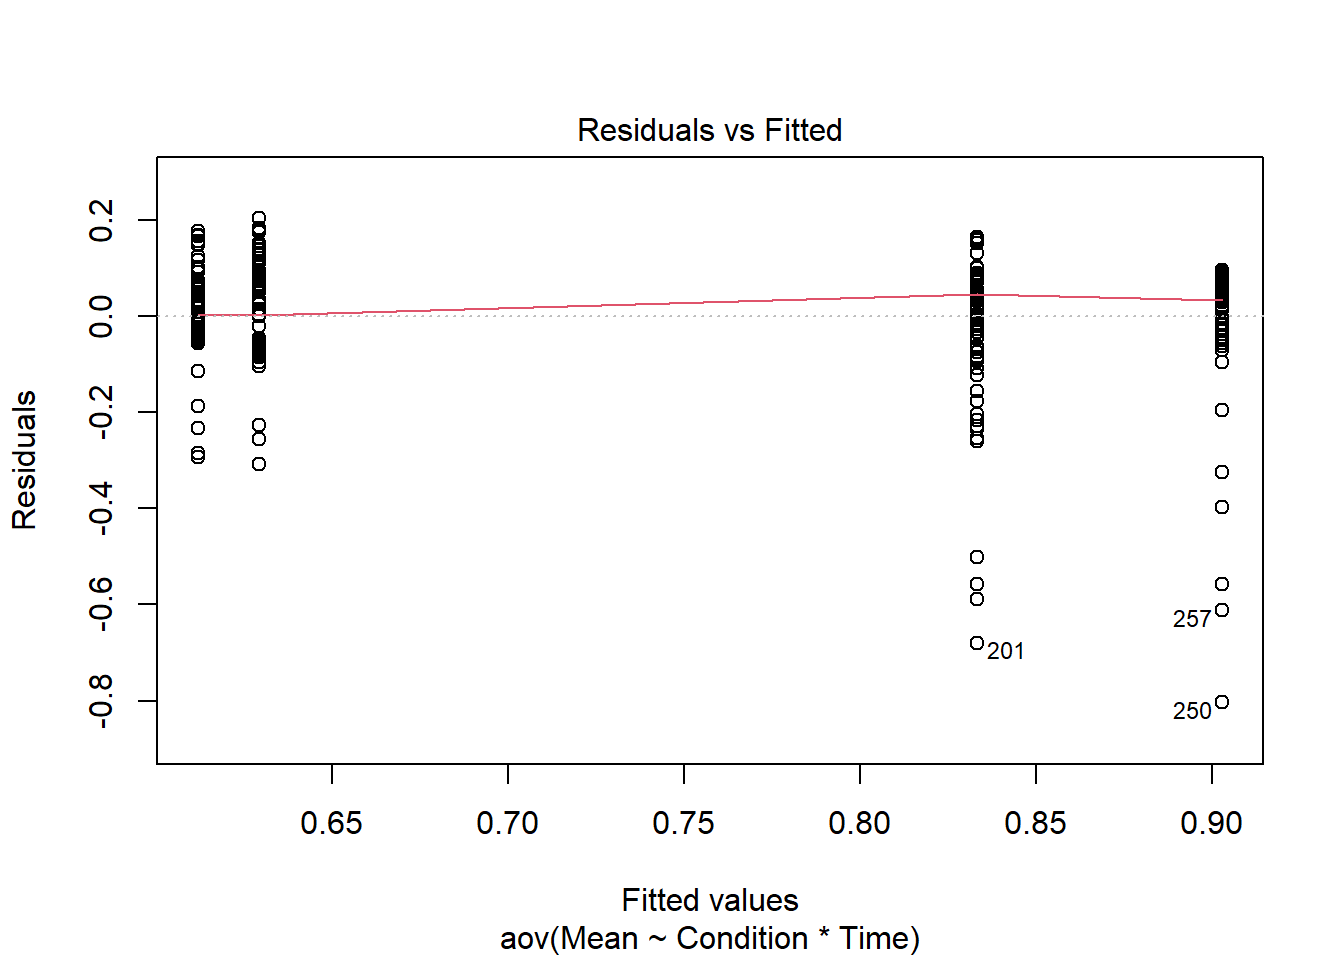
\includegraphics{ALL_TOGETHER_files/figure-latex/Performance-1}

\begin{Shaded}
\begin{Highlighting}[]
\DocumentationTok{\#\# NORMALITY}
\NormalTok{aov\_residuals }\OtherTok{\textless{}{-}} \FunctionTok{residuals}\NormalTok{ (}\AttributeTok{object=}\NormalTok{res.aov2)}
\FunctionTok{shapiro.test}\NormalTok{(}\AttributeTok{x=}\NormalTok{aov\_residuals) }\CommentTok{\# no normality! }
\end{Highlighting}
\end{Shaded}

\begin{verbatim}
## 
##  Shapiro-Wilk normality test
## 
## data:  aov_residuals
## W = 0.78526, p-value < 2.2e-16
\end{verbatim}

\begin{Shaded}
\begin{Highlighting}[]
\CommentTok{\# EXP \%\textgreater{}\%}
\CommentTok{\#   group\_by(Condition, Time) \%\textgreater{}\%}
\CommentTok{\#   shapiro.test(Mean) \# no normal distribution!}
\CommentTok{\#visualisation}
\FunctionTok{plot}\NormalTok{(res.aov2, }\DecValTok{2}\NormalTok{) }\CommentTok{\#clearly not normal}
\end{Highlighting}
\end{Shaded}

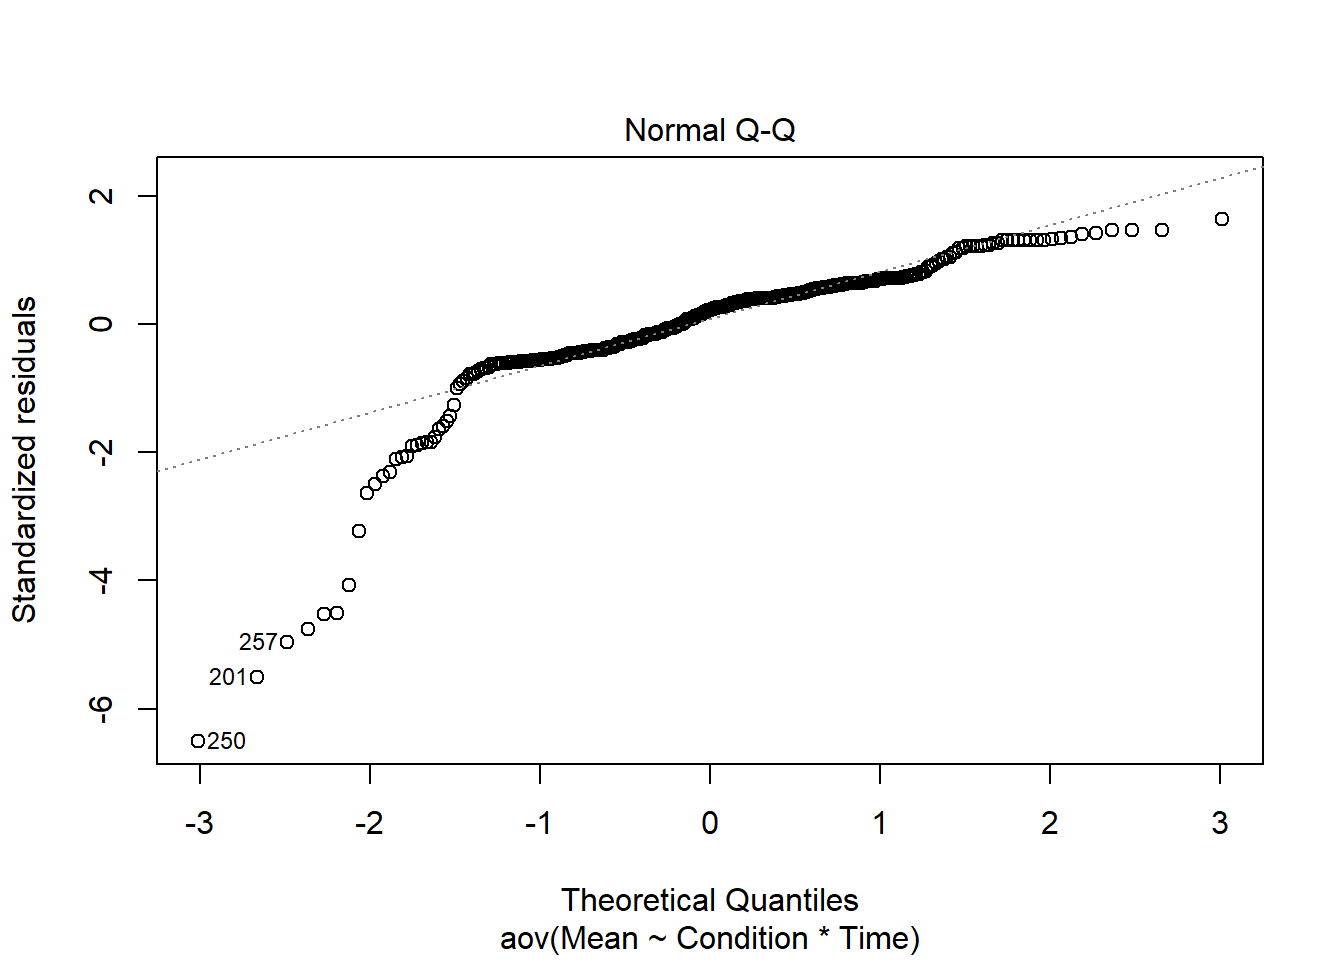
\includegraphics{ALL_TOGETHER_files/figure-latex/Performance-2}

\begin{Shaded}
\begin{Highlighting}[]
\FunctionTok{ggqqplot}\NormalTok{(EXP, }\StringTok{"Mean"}\NormalTok{, }\AttributeTok{ggtheme =} \FunctionTok{theme\_bw}\NormalTok{()) }\SpecialCharTok{+}
  \FunctionTok{facet\_grid}\NormalTok{(Time }\SpecialCharTok{\textasciitilde{}}\NormalTok{ Condition)}
\end{Highlighting}
\end{Shaded}

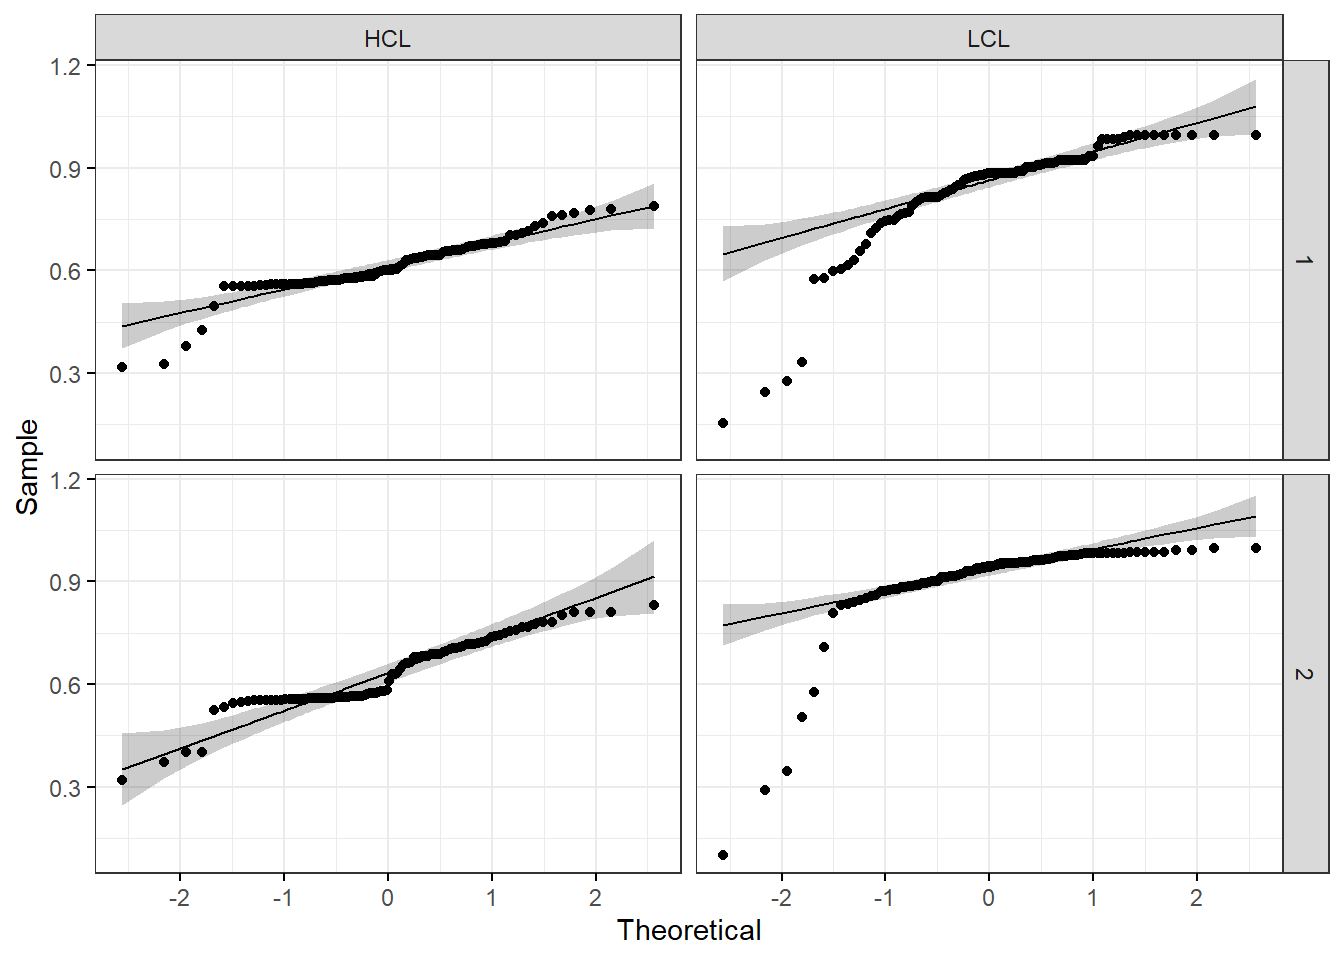
\includegraphics{ALL_TOGETHER_files/figure-latex/Performance-3}

\begin{Shaded}
\begin{Highlighting}[]
\FunctionTok{ggqqplot}\NormalTok{(EXP, }\StringTok{"Mean"}\NormalTok{, }\AttributeTok{ggtheme =} \FunctionTok{theme\_bw}\NormalTok{()) }\SpecialCharTok{+}
  \FunctionTok{facet\_grid}\NormalTok{( }\SpecialCharTok{\textasciitilde{}}\NormalTok{Condition) }\CommentTok{\#  very obviously NOT a normal distribution}
\end{Highlighting}
\end{Shaded}

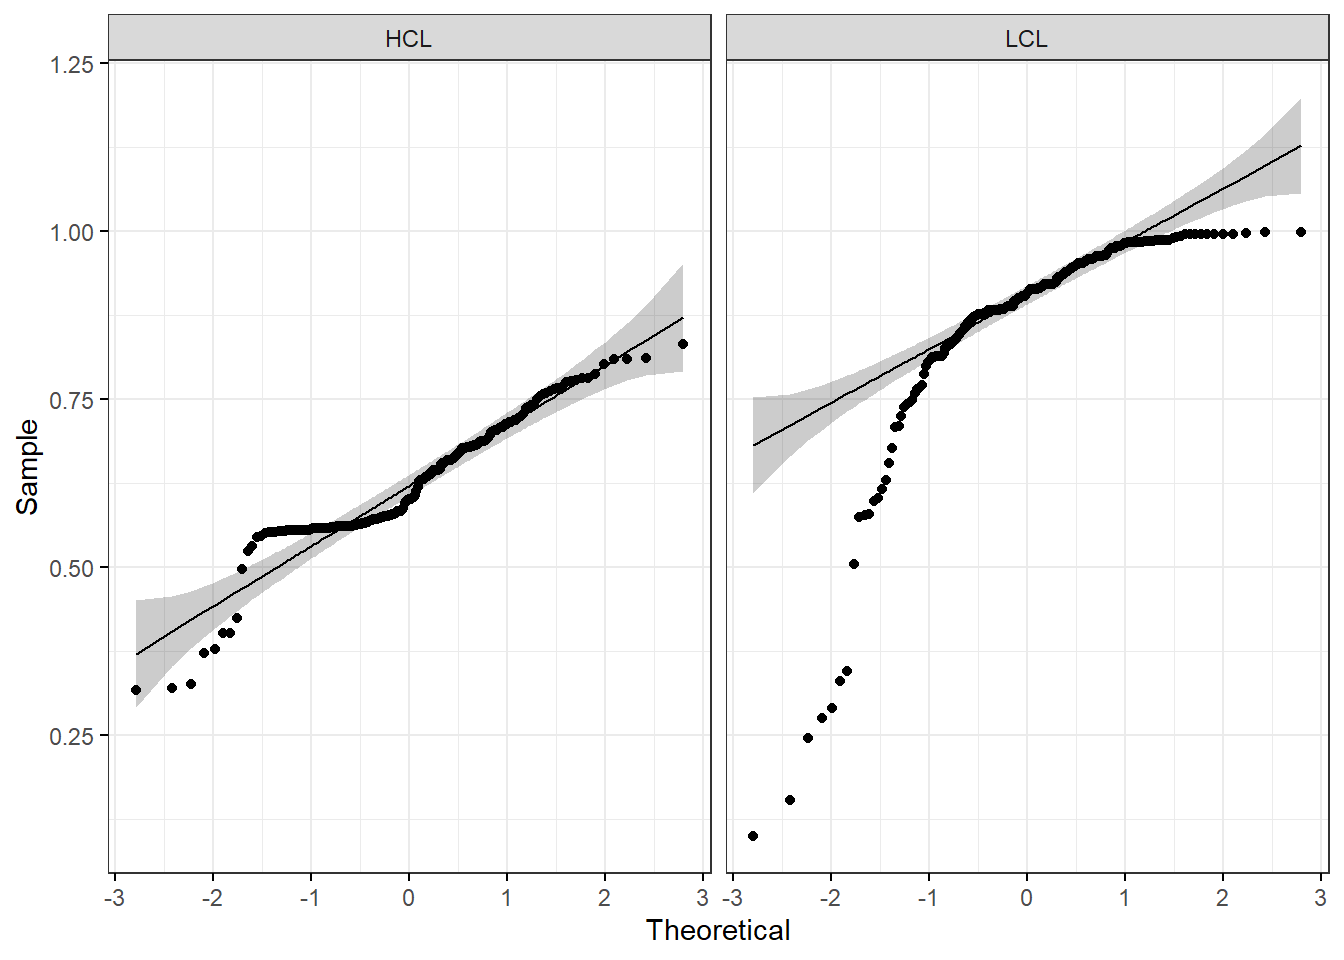
\includegraphics{ALL_TOGETHER_files/figure-latex/Performance-4}

\begin{Shaded}
\begin{Highlighting}[]
\DocumentationTok{\#\# SPHERICITY: Mauchly\textquotesingle{}s test}
\NormalTok{x}\OtherTok{\textless{}{-}}\FunctionTok{anova\_test}\NormalTok{(}\AttributeTok{data=}\NormalTok{ EXP, }\AttributeTok{dv=}\NormalTok{ Mean, }\AttributeTok{wid=}\NormalTok{ ID, }\AttributeTok{between=}\NormalTok{ Condition, }\AttributeTok{within=} \FunctionTok{c}\NormalTok{(Time, Day))}
\FunctionTok{get\_anova\_table}\NormalTok{(x, }\AttributeTok{correction =} \FunctionTok{c}\NormalTok{(}\StringTok{\textquotesingle{}GG\textquotesingle{}}\NormalTok{)) }\CommentTok{\#variances are NOT equal! }
\end{Highlighting}
\end{Shaded}

\begin{verbatim}
## ANOVA Table (type III tests)
## 
##               Effect DFn DFd       F        p p<.05   ges
## 1          Condition   1  95 162.886 2.56e-22     * 0.539
## 2               Time   1  95  93.602 8.19e-16     * 0.035
## 3                Day   1  95  24.982 2.64e-06     * 0.057
## 4     Condition:Time   1  95  34.272 6.82e-08     * 0.013
## 5      Condition:Day   1  95   2.729 1.02e-01       0.007
## 6           Time:Day   1  95  19.077 3.20e-05     * 0.010
## 7 Condition:Time:Day   1  95 158.069 6.30e-22     * 0.076
\end{verbatim}

\begin{Shaded}
\begin{Highlighting}[]
\NormalTok{x}\SpecialCharTok{$}\StringTok{\textquotesingle{}Sphericity Corrections\textquotesingle{}}
\end{Highlighting}
\end{Shaded}

\begin{verbatim}
## NULL
\end{verbatim}

\begin{Shaded}
\begin{Highlighting}[]
\DocumentationTok{\#\# OUTLIERS}
\NormalTok{EXP }\SpecialCharTok{\%\textgreater{}\%}
  \FunctionTok{group\_by}\NormalTok{(Condition, Time) }\SpecialCharTok{\%\textgreater{}\%}
  \FunctionTok{identify\_outliers}\NormalTok{(Mean)}
\end{Highlighting}
\end{Shaded}

\begin{verbatim}
## # A tibble: 21 x 8
##    Condition Time  Day   ID    count  Mean is.outlier is.extreme
##    <fct>     <fct> <fct> <fct> <int> <dbl> <lgl>      <lgl>     
##  1 HCL       1     1     63       44 0.326 TRUE       FALSE     
##  2 HCL       1     1     95       44 0.318 TRUE       FALSE     
##  3 HCL       1     2     63       44 0.425 TRUE       FALSE     
##  4 HCL       1     2     95       44 0.378 TRUE       FALSE     
##  5 HCL       2     2     95       52 0.320 TRUE       FALSE     
##  6 LCL       1     1     4        44 0.574 TRUE       FALSE     
##  7 LCL       1     1     9        44 0.153 TRUE       TRUE      
##  8 LCL       1     1     16       44 0.245 TRUE       TRUE      
##  9 LCL       1     1     20       44 0.598 TRUE       FALSE     
## 10 LCL       1     1     27       44 0.630 TRUE       FALSE     
## # ... with 11 more rows
\end{verbatim}

\begin{Shaded}
\begin{Highlighting}[]
\NormalTok{ outliers }\OtherTok{\textless{}{-}} \FunctionTok{boxplot}\NormalTok{(EXP}\SpecialCharTok{$}\NormalTok{prop\_correct, }\AttributeTok{plot=}\ConstantTok{FALSE}\NormalTok{)}\SpecialCharTok{$}\NormalTok{out}
\FunctionTok{summary}\NormalTok{(EXP}\SpecialCharTok{$}\NormalTok{Mean)}
\end{Highlighting}
\end{Shaded}

\begin{verbatim}
##    Min. 1st Qu.  Median    Mean 3rd Qu.    Max. 
##  0.0992  0.5827  0.7432  0.7460  0.9092  0.9985
\end{verbatim}

\begin{Shaded}
\begin{Highlighting}[]
\CommentTok{\#remove under e.g. 3? (sign not paying attention? a bit arbitrary)}
\CommentTok{\#EXP \textless{}{-}  EXP[!EXP$Mean\textless{}0.3,]}
\CommentTok{\#remove outliers per condition (HCL/LCL) because they have different distributions! }
\NormalTok{list\_quantiles }\OtherTok{\textless{}{-}} \FunctionTok{tapply}\NormalTok{(EXP}\SpecialCharTok{$}\NormalTok{Mean, EXP}\SpecialCharTok{$}\NormalTok{Condition, quantile)}
\NormalTok{Q1s }\OtherTok{\textless{}{-}} \FunctionTok{sapply}\NormalTok{(}\DecValTok{1}\SpecialCharTok{:}\DecValTok{2}\NormalTok{, }\ControlFlowTok{function}\NormalTok{(i) list\_quantiles[[i]][}\DecValTok{2}\NormalTok{])}
\NormalTok{Q3s }\OtherTok{\textless{}{-}} \FunctionTok{sapply}\NormalTok{(}\DecValTok{1}\SpecialCharTok{:}\DecValTok{2}\NormalTok{, }\ControlFlowTok{function}\NormalTok{(i) list\_quantiles[[i]][}\DecValTok{4}\NormalTok{])}
\NormalTok{IQRs }\OtherTok{\textless{}{-}} \FunctionTok{tapply}\NormalTok{(EXP}\SpecialCharTok{$}\NormalTok{Mean, EXP}\SpecialCharTok{$}\NormalTok{Condition, IQR)}
\NormalTok{Lowers }\OtherTok{\textless{}{-}}\NormalTok{ Q1s }\SpecialCharTok{{-}} \FloatTok{1.5}\SpecialCharTok{*}\NormalTok{IQRs}
\NormalTok{Uppers }\OtherTok{\textless{}{-}}\NormalTok{ Q3s }\SpecialCharTok{+} \FloatTok{1.5}\SpecialCharTok{*}\NormalTok{IQRs}
\NormalTok{datas }\OtherTok{\textless{}{-}} \FunctionTok{split}\NormalTok{(EXP, EXP}\SpecialCharTok{$}\NormalTok{Condition)}
\NormalTok{data\_no\_outlier }\OtherTok{\textless{}{-}} \ConstantTok{NULL}
\ControlFlowTok{for}\NormalTok{ (i }\ControlFlowTok{in} \DecValTok{1}\SpecialCharTok{:}\DecValTok{2}\NormalTok{)\{}
\NormalTok{  out }\OtherTok{\textless{}{-}} \FunctionTok{subset}\NormalTok{(datas[[i]], datas[[i]]}\SpecialCharTok{$}\NormalTok{Mean }\SpecialCharTok{\textgreater{}}\NormalTok{ Lowers[i] }\SpecialCharTok{\&}\NormalTok{ datas[[i]]}\SpecialCharTok{$}\NormalTok{Mean }\SpecialCharTok{\textless{}}\NormalTok{ Uppers[i])}
\NormalTok{  data\_no\_outlier }\OtherTok{\textless{}{-}} \FunctionTok{rbind}\NormalTok{(data\_no\_outlier, out)\}}
\NormalTok{EXP}\OtherTok{\textless{}{-}} \FunctionTok{as.data.frame}\NormalTok{(data\_no\_outlier)}
\CommentTok{\#even after log transform and removing outliers we have clearly not a normal distribution }
\CommentTok{\# so we need to use GLM. https://stats.stackexchange.com/questions/189115/fitting{-}a{-}binomial{-}glmm{-}glmer{-}to{-}a{-}response{-}variable{-}that{-}is{-}a{-}proportion{-}or{-}f}

\DocumentationTok{\#\#\# CONDITION * TIME }\AlertTok{\#\#\#}
\CommentTok{\# HCLvs LCL over time}
\CommentTok{\#BINOMIAL because the Mean accuracy is between 0 and 1}
\CommentTok{\# it is a (continuous) proportion: we need to use the \textquotesingle{}weights\textquotesingle{} argument for the number of trials that lead to the proportion}
\NormalTok{two\_w }\OtherTok{\textless{}{-}} \FunctionTok{glmer}\NormalTok{(Mean }\SpecialCharTok{\textasciitilde{}}\NormalTok{ Condition }\SpecialCharTok{*}\NormalTok{ Time }\SpecialCharTok{+}\NormalTok{ (}\DecValTok{1} \SpecialCharTok{|}\NormalTok{ ID), }\AttributeTok{weights =}\NormalTok{ count,}
   \AttributeTok{family =}\NormalTok{ binomial, }\AttributeTok{data =}\NormalTok{ EXP)}
\NormalTok{emmeans1}\OtherTok{\textless{}{-}} \FunctionTok{emmeans}\NormalTok{(two\_w, pairwise }\SpecialCharTok{\textasciitilde{}}\NormalTok{ Condition }\SpecialCharTok{*}\NormalTok{ Time, }\AttributeTok{adjust =}\StringTok{"fdr"}\NormalTok{, }\AttributeTok{type =} \StringTok{"response"}\NormalTok{)}
\NormalTok{emmean\_dataframe }\OtherTok{\textless{}{-}} \FunctionTok{summary}\NormalTok{(emmeans1)}\SpecialCharTok{$}\NormalTok{emmeans}
\FunctionTok{Anova}\NormalTok{(two\_w, }\AttributeTok{type=}\StringTok{\textquotesingle{}III\textquotesingle{}}\NormalTok{)}
\end{Highlighting}
\end{Shaded}

\begin{verbatim}
## Analysis of Deviance Table (Type III Wald chisquare tests)
## 
## Response: Mean
##                  Chisq Df Pr(>Chisq)    
## (Intercept)    113.856  1  < 2.2e-16 ***
## Condition      397.170  1  < 2.2e-16 ***
## Time            17.230  1  3.313e-05 ***
## Condition:Time  39.759  1  2.873e-10 ***
## ---
## Signif. codes:  0 '***' 0.001 '**' 0.01 '*' 0.05 '.' 0.1 ' ' 1
\end{verbatim}

\begin{Shaded}
\begin{Highlighting}[]
\FunctionTok{summary}\NormalTok{(emmeans1)}
\end{Highlighting}
\end{Shaded}

\begin{verbatim}
## $emmeans
##  Condition Time  prob      SE  df asymp.LCL asymp.UCL
##  HCL       1    0.617 0.01057 Inf     0.596     0.638
##  LCL       1    0.886 0.00655 Inf     0.872     0.898
##  HCL       2    0.642 0.01024 Inf     0.622     0.662
##  LCL       2    0.936 0.00445 Inf     0.927     0.944
## 
## Confidence level used: 0.95 
## Intervals are back-transformed from the logit scale 
## 
## $contrasts
##  contrast      odds.ratio      SE  df null z.ratio p.value
##  HCL 1 / LCL 1      0.208 0.01638 Inf    1 -19.929  <.0001
##  HCL 1 / HCL 2      0.898 0.02333 Inf    1  -4.151  <.0001
##  HCL 1 / LCL 2      0.110 0.00957 Inf    1 -25.317  <.0001
##  LCL 1 / HCL 2      4.326 0.34085 Inf    1  18.585  <.0001
##  LCL 1 / LCL 2      0.528 0.04227 Inf    1  -7.975  <.0001
##  HCL 2 / LCL 2      0.122 0.01065 Inf    1 -24.112  <.0001
## 
## P value adjustment: fdr method for 6 tests 
## Tests are performed on the log odds ratio scale
\end{verbatim}

\begin{Shaded}
\begin{Highlighting}[]
\CommentTok{\#summary }
\NormalTok{sum }\OtherTok{\textless{}{-}} \FunctionTok{sum\_2}\NormalTok{ (EXP, }\StringTok{\textquotesingle{}Time\textquotesingle{}}\NormalTok{, }\StringTok{\textquotesingle{}Condition\textquotesingle{}}\NormalTok{, }\StringTok{\textquotesingle{}Mean\textquotesingle{}}\NormalTok{)}
\NormalTok{sum}
\end{Highlighting}
\end{Shaded}

\begin{verbatim}
## # A tibble: 4 x 7
## # Groups:   Time [2]
##   Time  Condition     n  mean     sd      se     ic
##   <fct> <fct>     <int> <dbl>  <dbl>   <dbl>  <dbl>
## 1 1     HCL          93 0.621 0.0665 0.00690 0.0137
## 2 1     LCL          86 0.881 0.0734 0.00791 0.0157
## 3 2     HCL          94 0.635 0.0926 0.00955 0.0190
## 4 2     LCL          93 0.933 0.0513 0.00532 0.0106
\end{verbatim}

\begin{Shaded}
\begin{Highlighting}[]
\DocumentationTok{\#\# VISUALISATION}
\CommentTok{\# boxplot }
\NormalTok{bxp }\OtherTok{\textless{}{-}} \FunctionTok{ggboxplot}\NormalTok{(}
\NormalTok{  EXP, }\AttributeTok{x =} \StringTok{"Time"}\NormalTok{, }\AttributeTok{y =} \StringTok{"Mean"}\NormalTok{,}
  \AttributeTok{color =} \StringTok{"Condition"}\NormalTok{, }\AttributeTok{palette =} \StringTok{"jco"}\NormalTok{)}
\NormalTok{bxp}
\end{Highlighting}
\end{Shaded}

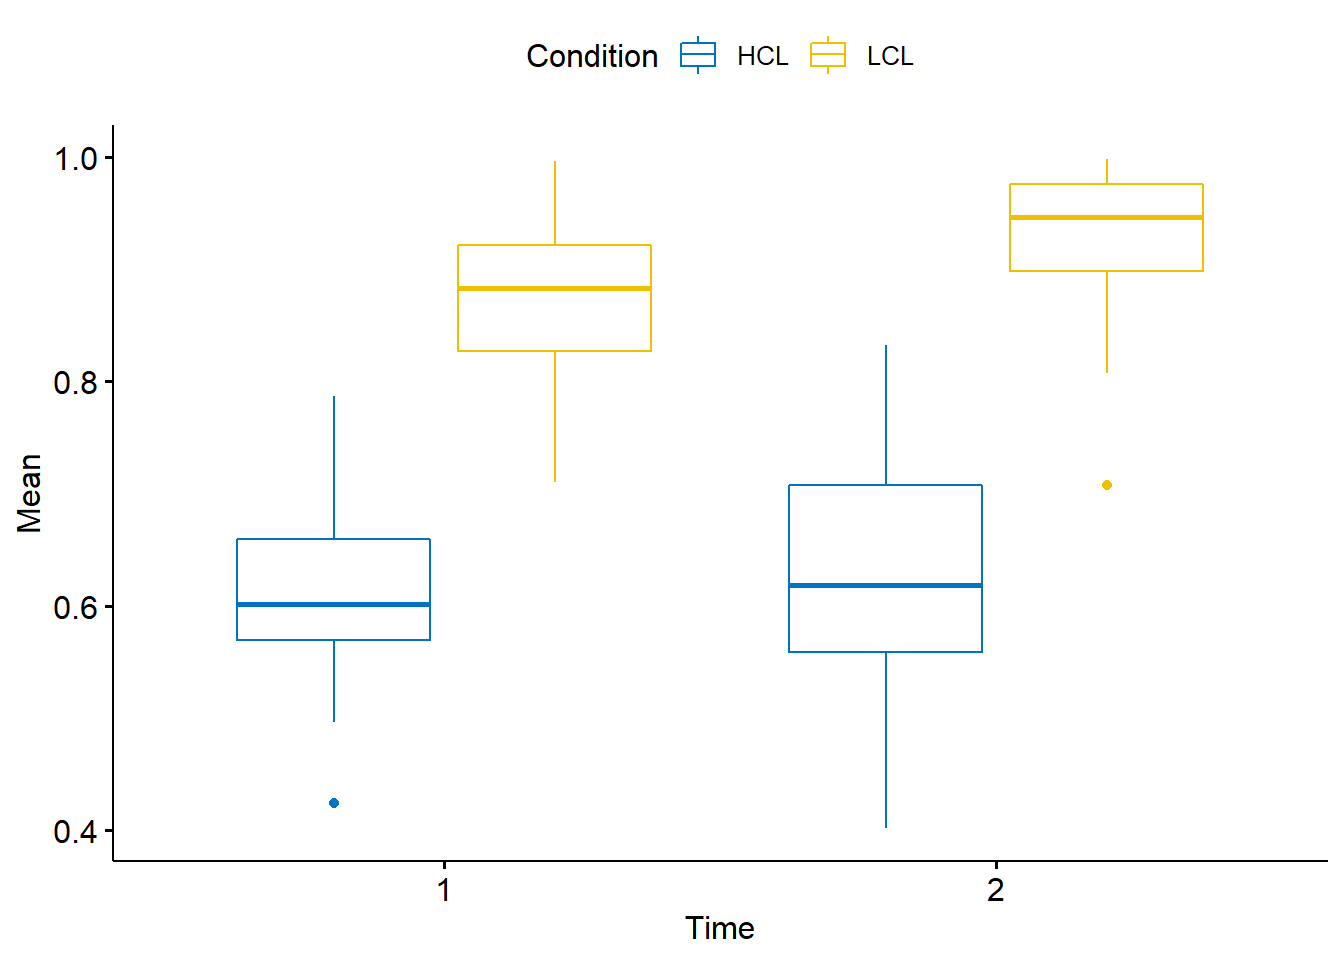
\includegraphics{ALL_TOGETHER_files/figure-latex/Performance-5}

\begin{Shaded}
\begin{Highlighting}[]
\NormalTok{max\_y}\OtherTok{\textless{}{-}}\FunctionTok{max}\NormalTok{(EXP}\SpecialCharTok{$}\NormalTok{Mean)}
\NormalTok{pl }\OtherTok{\textless{}{-}} \FunctionTok{plotty}\NormalTok{(EXP, emmean\_dataframe, }\StringTok{\textquotesingle{}Time\textquotesingle{}}\NormalTok{,  }\StringTok{\textquotesingle{}Mean\textquotesingle{}}\NormalTok{, }\StringTok{\textquotesingle{}Condition\textquotesingle{}}\NormalTok{, }\StringTok{\textquotesingle{}prob\textquotesingle{}}\NormalTok{, }\StringTok{\textquotesingle{}Performance/Objective CF\textquotesingle{}}\NormalTok{) }
  \CommentTok{\#   geom\_segment(aes(x =0.9, y = max\_y+max\_y/15, xend = 1.1, yend = max\_y+max\_y/15), size= 1)+ \# top line}
  \CommentTok{\# annotate(\textquotesingle{}text\textquotesingle{}, x=1, y=max\_y+max\_y/15+max\_y/100, label=\textquotesingle{}**\textquotesingle{}, size=7)+ \# tar}
  \CommentTok{\#   geom\_segment(aes(x =1.9, y = max\_y+max\_y/15, xend = 2.1, yend = max\_y+max\_y/15), size= 1) \# top line}
  \CommentTok{\# \# annotate(\textquotesingle{}text\textquotesingle{}, x=2, y=max\_y+max\_y/15+max\_y/100, label=\textquotesingle{}*\textquotesingle{}, size=7) \# star}
\FunctionTok{ggsave}\NormalTok{(pl, }\AttributeTok{file=}\FunctionTok{paste0}\NormalTok{(plotPrefix, }\StringTok{"Acc\_Cond\_Time\_Plot.jpg"}\NormalTok{), }\AttributeTok{width =} \DecValTok{2500}\NormalTok{, }\AttributeTok{height =} \DecValTok{1500}\NormalTok{, }\AttributeTok{dpi =} \DecValTok{300}\NormalTok{, }\AttributeTok{units =} \StringTok{"px"}\NormalTok{)}
\NormalTok{pl}
\end{Highlighting}
\end{Shaded}

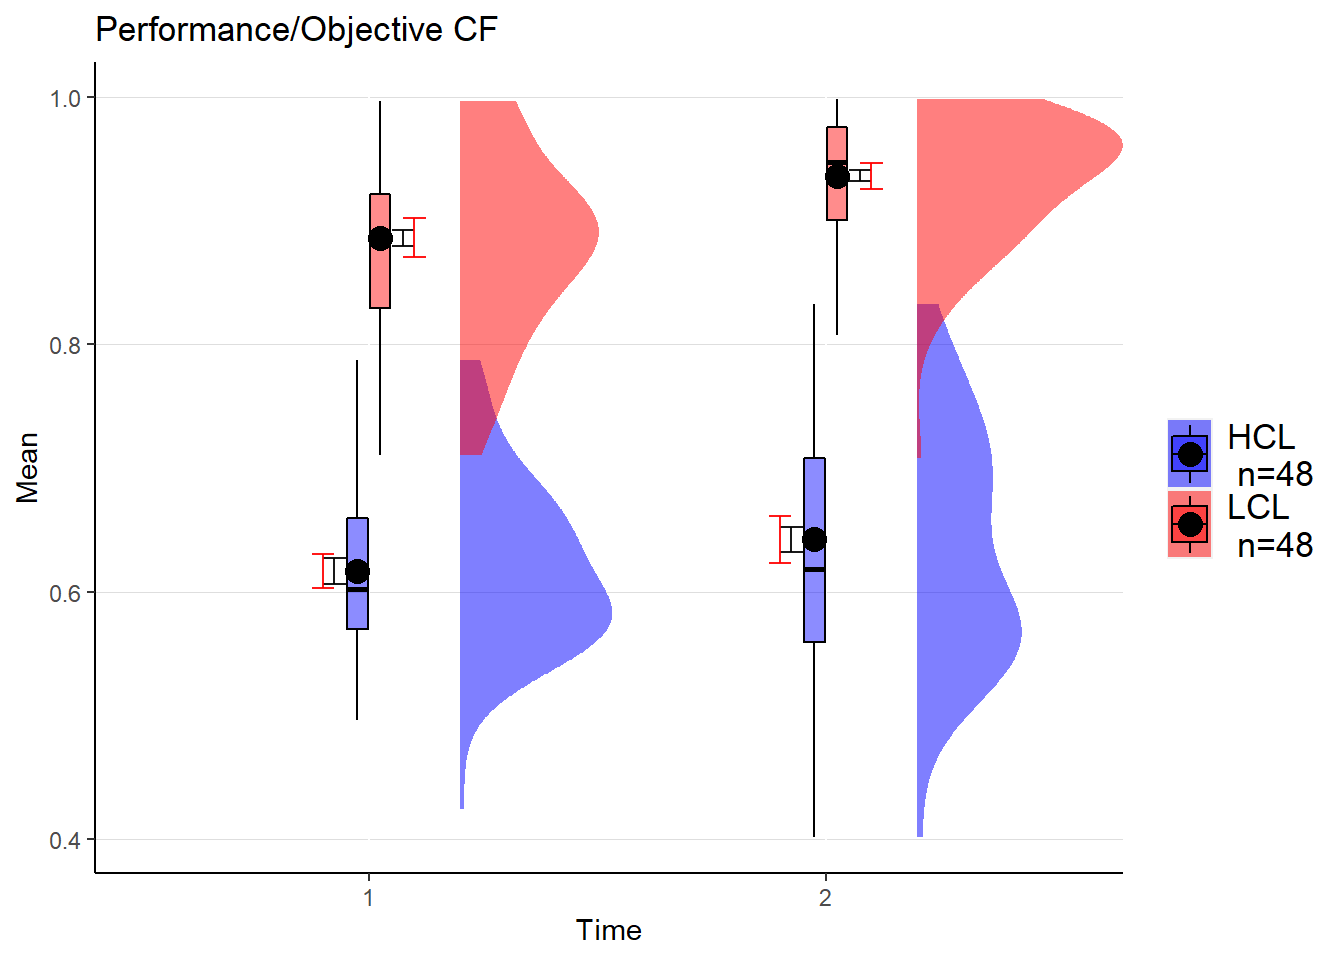
\includegraphics{ALL_TOGETHER_files/figure-latex/Performance-6}

\begin{Shaded}
\begin{Highlighting}[]
\DocumentationTok{\#\#\# CONDITION }\AlertTok{\#\#\#}
\NormalTok{one\_w }\OtherTok{\textless{}{-}} \FunctionTok{glmer}\NormalTok{(Mean }\SpecialCharTok{\textasciitilde{}}\NormalTok{ Condition  }\SpecialCharTok{+}\NormalTok{ (}\DecValTok{1} \SpecialCharTok{|}\NormalTok{ ID), }\AttributeTok{weights =}\NormalTok{ count,}
   \AttributeTok{family =}\NormalTok{ binomial, }\AttributeTok{data =}\NormalTok{ EXP)}
\NormalTok{emmeans1}\OtherTok{\textless{}{-}} \FunctionTok{emmeans}\NormalTok{(one\_w, pairwise }\SpecialCharTok{\textasciitilde{}}\NormalTok{ Condition, }\AttributeTok{adjust =}\StringTok{"fdr"}\NormalTok{, }\AttributeTok{type =} \StringTok{"response"}\NormalTok{)}
\NormalTok{emmean\_dataframe }\OtherTok{\textless{}{-}} \FunctionTok{summary}\NormalTok{(emmeans1)}\SpecialCharTok{$}\NormalTok{emmeans}

\FunctionTok{Anova}\NormalTok{(one\_w, }\AttributeTok{type=}\StringTok{\textquotesingle{}III\textquotesingle{}}\NormalTok{)}
\end{Highlighting}
\end{Shaded}

\begin{verbatim}
## Analysis of Deviance Table (Type III Wald chisquare tests)
## 
## Response: Mean
##              Chisq Df Pr(>Chisq)    
## (Intercept) 169.27  1  < 2.2e-16 ***
## Condition   685.42  1  < 2.2e-16 ***
## ---
## Signif. codes:  0 '***' 0.001 '**' 0.01 '*' 0.05 '.' 0.1 ' ' 1
\end{verbatim}

\begin{Shaded}
\begin{Highlighting}[]
\FunctionTok{summary}\NormalTok{(emmeans1)}\CommentTok{\# LCL clearly has higher Mean: 0.89 for LCL and 0.62 for HCL}
\end{Highlighting}
\end{Shaded}

\begin{verbatim}
## $emmeans
##  Condition  prob      SE  df asymp.LCL asymp.UCL
##  HCL       0.630 0.00955 Inf     0.611     0.649
##  LCL       0.912 0.00443 Inf     0.903     0.920
## 
## Confidence level used: 0.95 
## Intervals are back-transformed from the logit scale 
## 
## $contrasts
##  contrast  odds.ratio     SE  df null z.ratio p.value
##  HCL / LCL      0.164 0.0113 Inf    1 -26.180  <.0001
## 
## Tests are performed on the log odds ratio scale
\end{verbatim}

\begin{Shaded}
\begin{Highlighting}[]
\DocumentationTok{\#\#VISUALISATION}
\CommentTok{\# boxplot }
\NormalTok{bxp }\OtherTok{\textless{}{-}} \FunctionTok{ggboxplot}\NormalTok{(}
\NormalTok{  EXP, }\AttributeTok{x =} \StringTok{"Condition"}\NormalTok{, }\AttributeTok{y =} \StringTok{"Mean"}\NormalTok{, }\AttributeTok{palette =} \StringTok{"jco"}\NormalTok{)}
\NormalTok{bxp}
\end{Highlighting}
\end{Shaded}

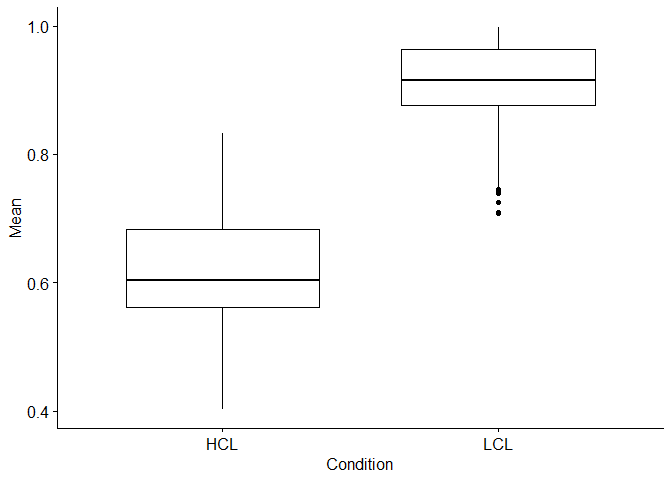
\includegraphics{ALL_TOGETHER_files/figure-latex/Performance-7}

\begin{Shaded}
\begin{Highlighting}[]
\CommentTok{\#  plot}
\NormalTok{pl }\OtherTok{\textless{}{-}} \FunctionTok{one\_w\_plot}\NormalTok{(EXP, emmean\_dataframe, }\StringTok{\textquotesingle{}Condition\textquotesingle{}}\NormalTok{, }\StringTok{\textquotesingle{}Mean\textquotesingle{}}\NormalTok{, }\StringTok{\textquotesingle{}prob\textquotesingle{}}\NormalTok{, }\StringTok{\textquotesingle{}Performance/Objective CF\textquotesingle{}}\NormalTok{)}
\FunctionTok{ggsave}\NormalTok{(pl, }\AttributeTok{file=}\FunctionTok{paste0}\NormalTok{(plotPrefix, }\StringTok{"Acc\_Cond\_Plot.jpg"}\NormalTok{), }\AttributeTok{width =} \DecValTok{2500}\NormalTok{, }\AttributeTok{height =} \DecValTok{1500}\NormalTok{, }\AttributeTok{dpi =} \DecValTok{300}\NormalTok{, }\AttributeTok{units =} \StringTok{"px"}\NormalTok{)}
\NormalTok{pl}
\end{Highlighting}
\end{Shaded}

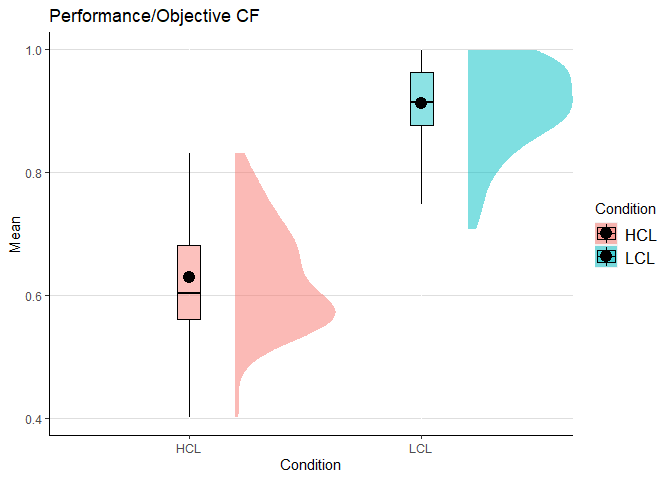
\includegraphics{ALL_TOGETHER_files/figure-latex/Performance-8}

\begin{Shaded}
\begin{Highlighting}[]
\DocumentationTok{\#\#\#\#  DAY 1 vs DAY 2 \#\#\#\#\#}
\NormalTok{two\_w }\OtherTok{\textless{}{-}} \FunctionTok{glmer}\NormalTok{(Mean }\SpecialCharTok{\textasciitilde{}}\NormalTok{ Condition }\SpecialCharTok{*}\NormalTok{ Day }\SpecialCharTok{+}\NormalTok{ (}\DecValTok{1} \SpecialCharTok{|}\NormalTok{ ID), }\AttributeTok{weights =}\NormalTok{ count,}
   \AttributeTok{family =}\NormalTok{ binomial, }\AttributeTok{data =}\NormalTok{ EXP)}
\NormalTok{emmeans1}\OtherTok{\textless{}{-}} \FunctionTok{emmeans}\NormalTok{(two\_w, pairwise }\SpecialCharTok{\textasciitilde{}}\NormalTok{ Condition }\SpecialCharTok{*}\NormalTok{ Day, }\AttributeTok{adjust =}\StringTok{"fdr"}\NormalTok{, }\AttributeTok{type =} \StringTok{"response"}\NormalTok{)}
\NormalTok{emmean\_dataframe }\OtherTok{\textless{}{-}} \FunctionTok{summary}\NormalTok{(emmeans1)}\SpecialCharTok{$}\NormalTok{emmeans}

\FunctionTok{Anova}\NormalTok{(two\_w, }\AttributeTok{type=}\StringTok{\textquotesingle{}III\textquotesingle{}}\NormalTok{)}
\end{Highlighting}
\end{Shaded}

\begin{verbatim}
## Analysis of Deviance Table (Type III Wald chisquare tests)
## 
## Response: Mean
##                  Chisq Df Pr(>Chisq)    
## (Intercept)    93.8420  1  < 2.2e-16 ***
## Condition     458.8108  1  < 2.2e-16 ***
## Day            54.6269  1  1.457e-13 ***
## Condition:Day   5.4124  1    0.01999 *  
## ---
## Signif. codes:  0 '***' 0.001 '**' 0.01 '*' 0.05 '.' 0.1 ' ' 1
\end{verbatim}

\begin{Shaded}
\begin{Highlighting}[]
\FunctionTok{summary}\NormalTok{(emmeans1)}
\end{Highlighting}
\end{Shaded}

\begin{verbatim}
## $emmeans
##  Condition Day  prob      SE  df asymp.LCL asymp.UCL
##  HCL       1   0.605 0.01053 Inf     0.584     0.626
##  LCL       1   0.895 0.00627 Inf     0.882     0.907
##  HCL       2   0.650 0.00988 Inf     0.631     0.669
##  LCL       2   0.926 0.00476 Inf     0.916     0.935
## 
## Confidence level used: 0.95 
## Intervals are back-transformed from the logit scale 
## 
## $contrasts
##  contrast      odds.ratio     SE  df null z.ratio p.value
##  HCL 1 / LCL 1      0.179 0.0144 Inf    1 -21.420  <.0001
##  HCL 1 / HCL 2      0.824 0.0216 Inf    1  -7.391  <.0001
##  HCL 1 / LCL 2      0.122 0.0101 Inf    1 -25.460  <.0001
##  LCL 1 / HCL 2      4.591 0.3666 Inf    1  19.089  <.0001
##  LCL 1 / LCL 2      0.680 0.0532 Inf    1  -4.932  <.0001
##  HCL 2 / LCL 2      0.148 0.0122 Inf    1 -23.214  <.0001
## 
## P value adjustment: fdr method for 6 tests 
## Tests are performed on the log odds ratio scale
\end{verbatim}

\begin{Shaded}
\begin{Highlighting}[]
\CommentTok{\#summary  }
\NormalTok{sum }\OtherTok{\textless{}{-}} \FunctionTok{sum\_2}\NormalTok{ (EXP, }\StringTok{\textquotesingle{}Day\textquotesingle{}}\NormalTok{, }\StringTok{\textquotesingle{}Condition\textquotesingle{}}\NormalTok{, }\StringTok{\textquotesingle{}Mean\textquotesingle{}}\NormalTok{)}
\NormalTok{sum}
\end{Highlighting}
\end{Shaded}

\begin{verbatim}
## # A tibble: 4 x 7
## # Groups:   Day [2]
##   Day   Condition     n  mean     sd      se     ic
##   <fct> <fct>     <int> <dbl>  <dbl>   <dbl>  <dbl>
## 1 1     HCL          94 0.608 0.0695 0.00716 0.0142
## 2 1     LCL          84 0.893 0.0731 0.00798 0.0159
## 3 2     HCL          93 0.649 0.0864 0.00896 0.0178
## 4 2     LCL          95 0.922 0.0601 0.00617 0.0123
\end{verbatim}

\begin{Shaded}
\begin{Highlighting}[]
\DocumentationTok{\#\# VISUALISATION}
\CommentTok{\# plot with error bars}
\NormalTok{pl }\OtherTok{\textless{}{-}} \FunctionTok{plotty}\NormalTok{(EXP, emmean\_dataframe, }\StringTok{\textquotesingle{}Day\textquotesingle{}}\NormalTok{,  }\StringTok{\textquotesingle{}Mean\textquotesingle{}}\NormalTok{, }\StringTok{\textquotesingle{}Condition\textquotesingle{}}\NormalTok{, }\StringTok{\textquotesingle{}prob\textquotesingle{}}\NormalTok{, }\StringTok{\textquotesingle{}Perfromance/Objective CF\textquotesingle{}}\NormalTok{) }
\FunctionTok{ggsave}\NormalTok{(pl, }\AttributeTok{file=}\FunctionTok{paste0}\NormalTok{(plotPrefix, }\StringTok{"Acc\_Cond\_Day\_Plot.jpg"}\NormalTok{), }\AttributeTok{width =} \DecValTok{2500}\NormalTok{, }\AttributeTok{height =} \DecValTok{1500}\NormalTok{, }\AttributeTok{dpi =} \DecValTok{300}\NormalTok{, }\AttributeTok{units =} \StringTok{"px"}\NormalTok{)}
\NormalTok{pl}
\end{Highlighting}
\end{Shaded}

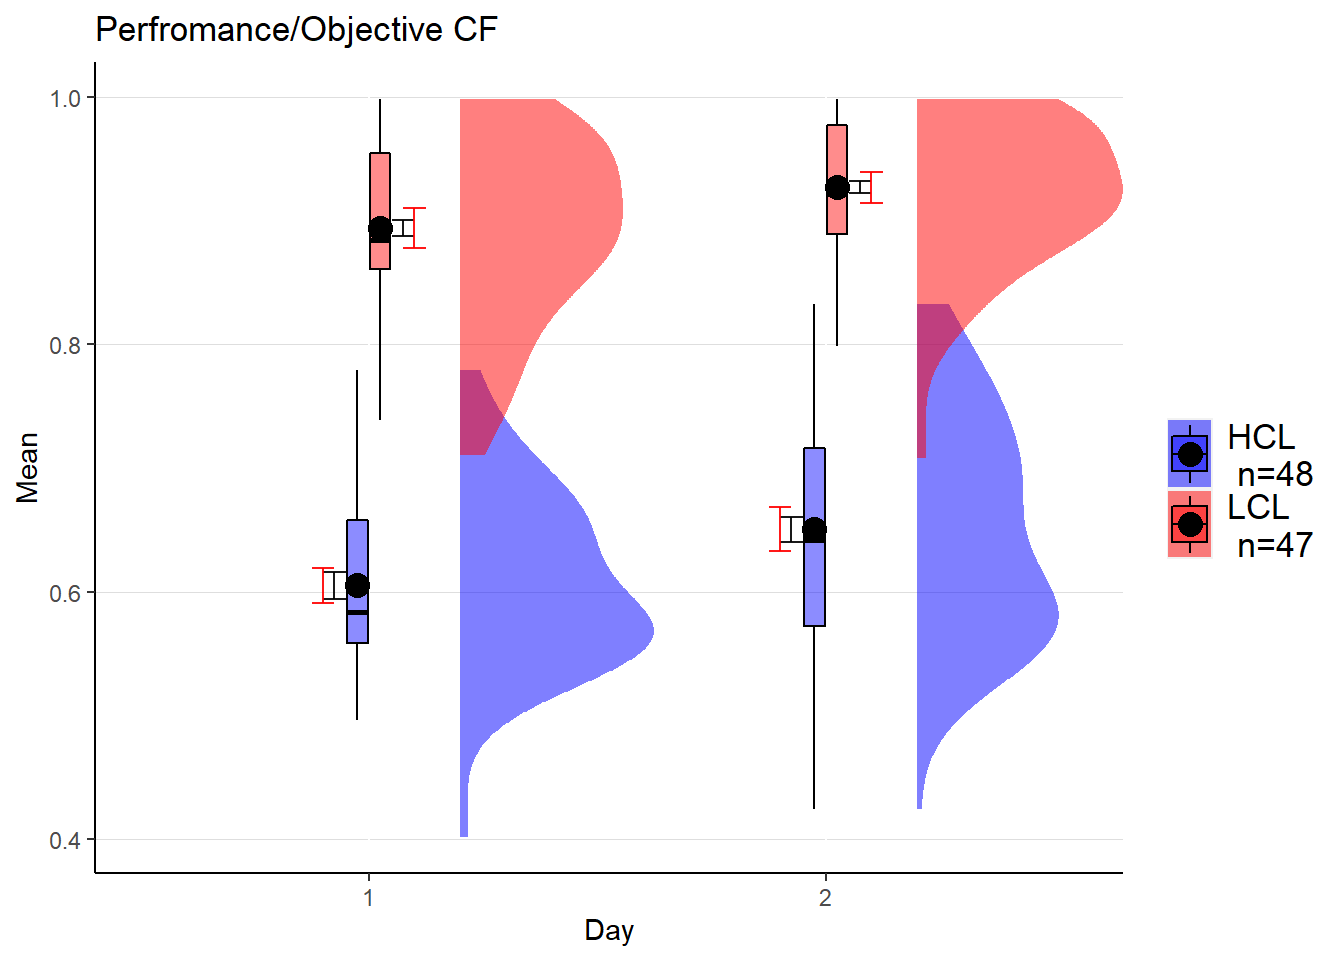
\includegraphics{ALL_TOGETHER_files/figure-latex/Performance-9}

\begin{Shaded}
\begin{Highlighting}[]
\DocumentationTok{\#\#\# Condition * Time * Day}
\NormalTok{three\_w }\OtherTok{\textless{}{-}} \FunctionTok{glmer}\NormalTok{(Mean }\SpecialCharTok{\textasciitilde{}}\NormalTok{ Condition }\SpecialCharTok{*}\NormalTok{ Time }\SpecialCharTok{*}\NormalTok{ Day }\SpecialCharTok{+}\NormalTok{ (}\DecValTok{1} \SpecialCharTok{|}\NormalTok{ ID), }\AttributeTok{weights =}\NormalTok{ count,}
   \AttributeTok{family =}\NormalTok{ binomial, }\AttributeTok{data =}\NormalTok{ EXP)}
\NormalTok{emmeans1}\OtherTok{\textless{}{-}} \FunctionTok{emmeans}\NormalTok{(three\_w, pairwise }\SpecialCharTok{\textasciitilde{}}\NormalTok{ Condition }\SpecialCharTok{*}\NormalTok{ Time }\SpecialCharTok{*}\NormalTok{ Day, }\AttributeTok{adjust =}\StringTok{"fdr"}\NormalTok{, }\AttributeTok{type =} \StringTok{"response"}\NormalTok{)}
\NormalTok{emmean\_dataframe }\OtherTok{\textless{}{-}} \FunctionTok{summary}\NormalTok{(emmeans1)}\SpecialCharTok{$}\NormalTok{emmeans}
\FunctionTok{Anova}\NormalTok{(two\_w, }\AttributeTok{type=}\StringTok{\textquotesingle{}III\textquotesingle{}}\NormalTok{)}
\end{Highlighting}
\end{Shaded}

\begin{verbatim}
## Analysis of Deviance Table (Type III Wald chisquare tests)
## 
## Response: Mean
##                  Chisq Df Pr(>Chisq)    
## (Intercept)    93.8420  1  < 2.2e-16 ***
## Condition     458.8108  1  < 2.2e-16 ***
## Day            54.6269  1  1.457e-13 ***
## Condition:Day   5.4124  1    0.01999 *  
## ---
## Signif. codes:  0 '***' 0.001 '**' 0.01 '*' 0.05 '.' 0.1 ' ' 1
\end{verbatim}

\begin{Shaded}
\begin{Highlighting}[]
\FunctionTok{summary}\NormalTok{(emmeans1)}
\end{Highlighting}
\end{Shaded}

\begin{verbatim}
## $emmeans
##  Condition Time Day  prob      SE  df asymp.LCL asymp.UCL
##  HCL       1    1   0.650 0.01164 Inf     0.627     0.672
##  LCL       1    1   0.844 0.01066 Inf     0.822     0.864
##  HCL       2    1   0.562 0.01234 Inf     0.538     0.586
##  LCL       2    1   0.936 0.00595 Inf     0.923     0.947
##  HCL       1    2   0.592 0.01187 Inf     0.569     0.615
##  LCL       1    2   0.917 0.00670 Inf     0.903     0.929
##  HCL       2    2   0.707 0.01034 Inf     0.687     0.727
##  LCL       2    2   0.937 0.00572 Inf     0.925     0.947
## 
## Confidence level used: 0.95 
## Intervals are back-transformed from the logit scale 
## 
## $contrasts
##  contrast          odds.ratio      SE  df null z.ratio p.value
##  HCL 1 1 / LCL 1 1     0.3434 0.03284 Inf    1 -11.178  <.0001
##  HCL 1 1 / HCL 2 1     1.4428 0.05581 Inf    1   9.475  <.0001
##  HCL 1 1 / LCL 2 1     0.1270 0.01420 Inf    1 -18.461  <.0001
##  HCL 1 1 / HCL 1 2     1.2761 0.04758 Inf    1   6.538  <.0001
##  HCL 1 1 / LCL 1 2     0.1681 0.01713 Inf    1 -17.496  <.0001
##  HCL 1 1 / HCL 2 2     0.7672 0.02938 Inf    1  -6.919  <.0001
##  HCL 1 1 / LCL 2 2     0.1246 0.01367 Inf    1 -18.979  <.0001
##  LCL 1 1 / HCL 2 1     4.2014 0.39953 Inf    1  15.095  <.0001
##  LCL 1 1 / LCL 2 1     0.3698 0.04171 Inf    1  -8.819  <.0001
##  LCL 1 1 / HCL 1 2     3.7160 0.35145 Inf    1  13.879  <.0001
##  LCL 1 1 / LCL 1 2     0.4894 0.05081 Inf    1  -6.883  <.0001
##  LCL 1 1 / HCL 2 2     2.2342 0.21222 Inf    1   8.464  <.0001
##  LCL 1 1 / LCL 2 2     0.3629 0.04039 Inf    1  -9.107  <.0001
##  HCL 2 1 / LCL 2 1     0.0880 0.00979 Inf    1 -21.839  <.0001
##  HCL 2 1 / HCL 1 2     0.8845 0.03202 Inf    1  -3.391  0.0008
##  HCL 2 1 / LCL 1 2     0.1165 0.01181 Inf    1 -21.207  <.0001
##  HCL 2 1 / HCL 2 2     0.5318 0.01983 Inf    1 -16.935  <.0001
##  HCL 2 1 / LCL 2 2     0.0864 0.00943 Inf    1 -22.422  <.0001
##  LCL 2 1 / HCL 1 2    10.0494 1.11391 Inf    1  20.818  <.0001
##  LCL 2 1 / LCL 1 2     1.3236 0.15455 Inf    1   2.401  0.0170
##  LCL 2 1 / HCL 2 2     6.0422 0.67176 Inf    1  16.179  <.0001
##  LCL 2 1 / LCL 2 2     0.9814 0.12169 Inf    1  -0.151  0.8797
##  HCL 1 2 / LCL 1 2     0.1317 0.01329 Inf    1 -20.091  <.0001
##  HCL 1 2 / HCL 2 2     0.6013 0.02142 Inf    1 -14.279  <.0001
##  HCL 1 2 / LCL 2 2     0.0977 0.01062 Inf    1 -21.386  <.0001
##  LCL 1 2 / HCL 2 2     4.5650 0.46229 Inf    1  14.994  <.0001
##  LCL 1 2 / LCL 2 2     0.7415 0.08582 Inf    1  -2.584  0.0105
##  HCL 2 2 / LCL 2 2     0.1624 0.01772 Inf    1 -16.656  <.0001
## 
## P value adjustment: fdr method for 28 tests 
## Tests are performed on the log odds ratio scale
\end{verbatim}

\begin{Shaded}
\begin{Highlighting}[]
\DocumentationTok{\#\# plot with error bars}
\NormalTok{max\_y}\OtherTok{\textless{}{-}}\FunctionTok{max}\NormalTok{(EXP}\SpecialCharTok{$}\NormalTok{Mean)}
\NormalTok{pl }\OtherTok{\textless{}{-}} \FunctionTok{plotty}\NormalTok{(EXP, emmean\_dataframe, }\StringTok{\textquotesingle{}Time\textquotesingle{}}\NormalTok{,  }\StringTok{\textquotesingle{}Mean\textquotesingle{}}\NormalTok{, }\StringTok{\textquotesingle{}Condition\textquotesingle{}}\NormalTok{, }\StringTok{\textquotesingle{}prob\textquotesingle{}}\NormalTok{, }\StringTok{\textquotesingle{}Performance/Objective CF\textquotesingle{}}\NormalTok{) }\SpecialCharTok{+}
  \FunctionTok{facet\_grid}\NormalTok{(.}\SpecialCharTok{\textasciitilde{}}\NormalTok{Day)}
  \CommentTok{\#   geom\_segment(aes(x =0.9, y = max\_y+max\_y/15, xend = 1.1, yend = max\_y+max\_y/15), size= 1)+ \# top line}
  \CommentTok{\# annotate(\textquotesingle{}text\textquotesingle{}, x=1, y=max\_y+max\_y/15+max\_y/100, label=\textquotesingle{}**\textquotesingle{}, size=7)+ \# tar}
  \CommentTok{\#   geom\_segment(aes(x =1.9, y = max\_y+max\_y/15, xend = 2.1, yend = max\_y+max\_y/15), size= 1) \# top line}
  \CommentTok{\# \# annotate(\textquotesingle{}text\textquotesingle{}, x=2, y=max\_y+max\_y/15+max\_y/100, label=\textquotesingle{}*\textquotesingle{}, size=7) \# star}
\FunctionTok{ggsave}\NormalTok{(pl, }\AttributeTok{file=}\FunctionTok{paste0}\NormalTok{(plotPrefix, }\StringTok{"Acc\_Cond\_Time\_Plot.jpg"}\NormalTok{), }\AttributeTok{width =} \DecValTok{2500}\NormalTok{, }\AttributeTok{height =} \DecValTok{1500}\NormalTok{, }\AttributeTok{dpi =} \DecValTok{300}\NormalTok{, }\AttributeTok{units =} \StringTok{"px"}\NormalTok{)}
\NormalTok{pl}
\end{Highlighting}
\end{Shaded}

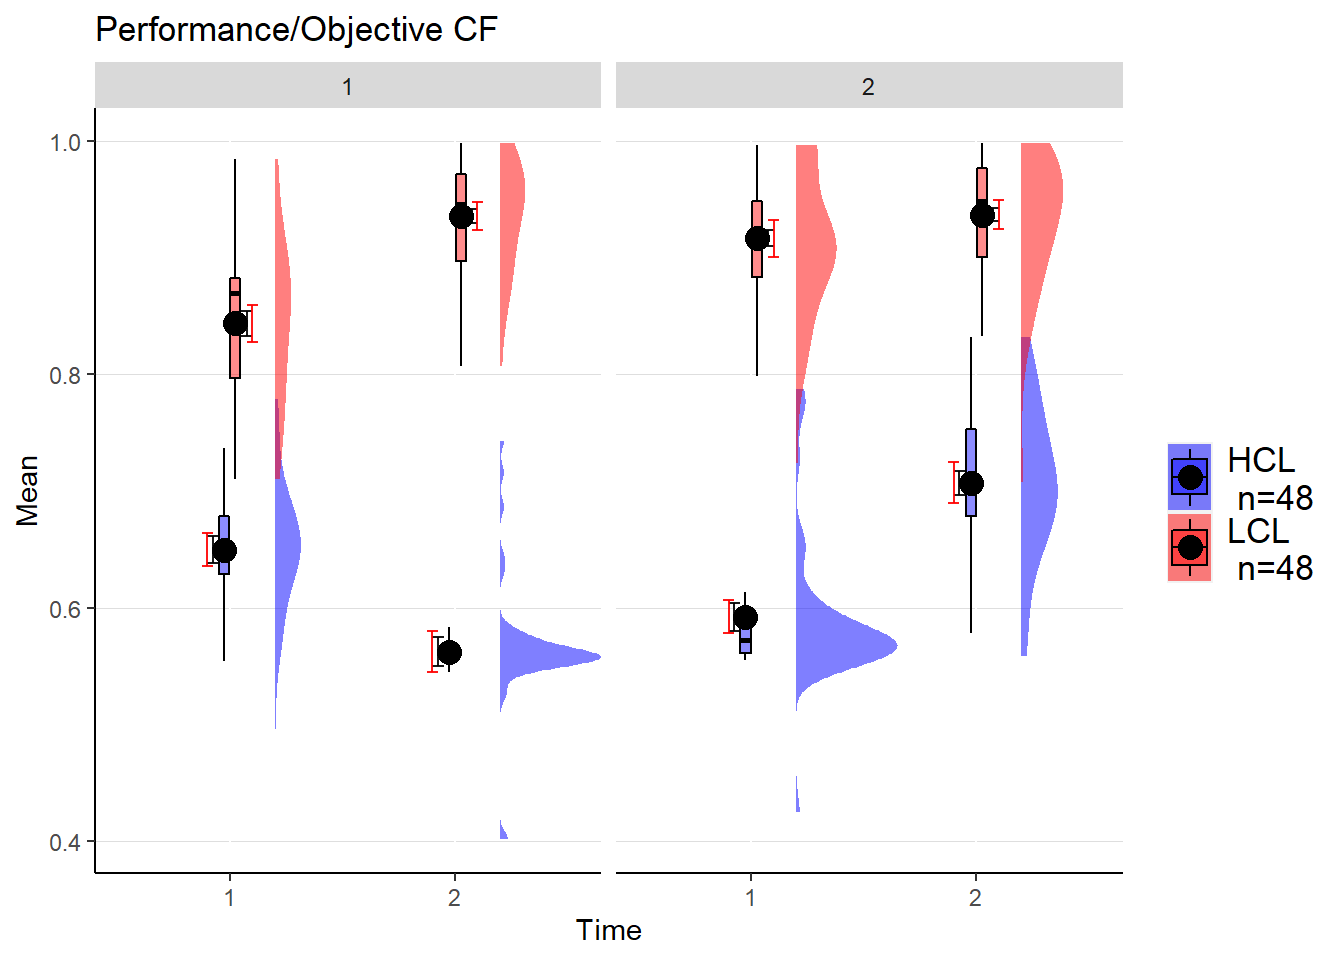
\includegraphics{ALL_TOGETHER_files/figure-latex/Performance-10}

\begin{Shaded}
\begin{Highlighting}[]
\DocumentationTok{\#\#\# COMPONENTS (Color/Pic)\#\#\#\#}

\CommentTok{\# evolution over time for 2 components of the task}
\CommentTok{\# Pics: decide if big/small. Color: decide if same as DualBack: more Working Memory}
\NormalTok{EXP1 }\OtherTok{\textless{}{-}} \FunctionTok{as.data.frame}\NormalTok{ (}\FunctionTok{group\_by}\NormalTok{(data, Condition, Day, Time, ID, Stim) }\SpecialCharTok{\%\textgreater{}\%}
  \FunctionTok{summarise}\NormalTok{(}
    \AttributeTok{count =} \FunctionTok{n}\NormalTok{(),}
    \AttributeTok{Mean =} \FunctionTok{mean}\NormalTok{(prop\_correct, }\AttributeTok{na.rm =} \ConstantTok{TRUE}\NormalTok{)}
\NormalTok{  ))}
\CommentTok{\# set factors}
\NormalTok{EXP1}\SpecialCharTok{$}\NormalTok{Time }\OtherTok{\textless{}{-}} \FunctionTok{as.factor}\NormalTok{(EXP1}\SpecialCharTok{$}\NormalTok{Time)}
\NormalTok{EXP1}\SpecialCharTok{$}\NormalTok{Condition }\OtherTok{\textless{}{-}} \FunctionTok{as.factor}\NormalTok{(EXP1}\SpecialCharTok{$}\NormalTok{Condition)}
\NormalTok{EXP1}\SpecialCharTok{$}\NormalTok{Day }\OtherTok{\textless{}{-}} \FunctionTok{as.factor}\NormalTok{(EXP1}\SpecialCharTok{$}\NormalTok{Day)}
\NormalTok{EXP1}\SpecialCharTok{$}\NormalTok{ID }\OtherTok{\textless{}{-}} \FunctionTok{as.factor}\NormalTok{(EXP1}\SpecialCharTok{$}\NormalTok{ID)}
\NormalTok{EXP1}\SpecialCharTok{$}\NormalTok{Stim }\OtherTok{\textless{}{-}} \FunctionTok{as.factor}\NormalTok{(EXP1}\SpecialCharTok{$}\NormalTok{Stim)}

\DocumentationTok{\#\# STATISTICAL }\AlertTok{TEST}
\NormalTok{three\_w }\OtherTok{\textless{}{-}} \FunctionTok{glmer}\NormalTok{(Mean }\SpecialCharTok{\textasciitilde{}}\NormalTok{ Condition }\SpecialCharTok{*}\NormalTok{ Time }\SpecialCharTok{*}\NormalTok{ Stim }\SpecialCharTok{+}\NormalTok{ (}\DecValTok{1} \SpecialCharTok{|}\NormalTok{ ID), }\AttributeTok{weights =}\NormalTok{ count,}
   \AttributeTok{family =}\NormalTok{ binomial, }\AttributeTok{data =}\NormalTok{ EXP1)}
\NormalTok{emmeans1}\OtherTok{\textless{}{-}} \FunctionTok{emmeans}\NormalTok{(three\_w, pairwise }\SpecialCharTok{\textasciitilde{}}\NormalTok{ Condition }\SpecialCharTok{*}\NormalTok{ Time }\SpecialCharTok{*}\NormalTok{ Stim, }\AttributeTok{adjust =}\StringTok{"fdr"}\NormalTok{, }\AttributeTok{type =} \StringTok{"response"}\NormalTok{)}
\NormalTok{emmean\_dataframe }\OtherTok{\textless{}{-}} \FunctionTok{summary}\NormalTok{(emmeans1)}\SpecialCharTok{$}\NormalTok{emmeans}

\FunctionTok{Anova}\NormalTok{(three\_w, }\AttributeTok{type=}\StringTok{\textquotesingle{}III\textquotesingle{}}\NormalTok{)}
\end{Highlighting}
\end{Shaded}

\begin{verbatim}
## Analysis of Deviance Table (Type III Wald chisquare tests)
## 
## Response: Mean
##                        Chisq Df Pr(>Chisq)    
## (Intercept)          27.5233  1  1.552e-07 ***
## Condition           107.5407  1  < 2.2e-16 ***
## Time                  8.6023  1   0.003357 ** 
## Stim                  0.1552  1   0.693569    
## Condition:Time       26.2623  1  2.981e-07 ***
## Condition:Stim        2.5317  1   0.111578    
## Time:Stim             0.0014  1   0.970086    
## Condition:Time:Stim   0.2982  1   0.585018    
## ---
## Signif. codes:  0 '***' 0.001 '**' 0.01 '*' 0.05 '.' 0.1 ' ' 1
\end{verbatim}

\begin{Shaded}
\begin{Highlighting}[]
\FunctionTok{summary}\NormalTok{(emmeans1)}
\end{Highlighting}
\end{Shaded}

\begin{verbatim}
## $emmeans
##  Condition Time Stim   prob      SE  df asymp.LCL asymp.UCL
##  HCL       1    Color 0.615 0.02107 Inf     0.573     0.655
##  LCL       1    Color 0.870 0.01196 Inf     0.844     0.891
##  HCL       2    Color 0.640 0.02049 Inf     0.599     0.679
##  LCL       2    Color 0.927 0.00779 Inf     0.910     0.941
##  HCL       1    Pic   0.611 0.02113 Inf     0.569     0.652
##  LCL       1    Pic   0.850 0.01321 Inf     0.822     0.874
##  HCL       2    Pic   0.636 0.02058 Inf     0.595     0.675
##  LCL       2    Pic   0.921 0.00829 Inf     0.904     0.936
## 
## Confidence level used: 0.95 
## Intervals are back-transformed from the logit scale 
## 
## $contrasts
##  contrast                  odds.ratio     SE  df null z.ratio p.value
##  HCL 1 Color / LCL 1 Color      0.239 0.0330 Inf    1 -10.370  <.0001
##  HCL 1 Color / HCL 2 Color      0.898 0.0329 Inf    1  -2.933  0.0043
##  HCL 1 Color / LCL 2 Color      0.125 0.0182 Inf    1 -14.261  <.0001
##  HCL 1 Color / HCL 1 Pic        1.015 0.0372 Inf    1   0.394  0.6936
##  HCL 1 Color / LCL 1 Pic        0.281 0.0384 Inf    1  -9.292  <.0001
##  HCL 1 Color / HCL 2 Pic        0.913 0.0334 Inf    1  -2.486  0.0151
##  HCL 1 Color / LCL 2 Pic        0.136 0.0197 Inf    1 -13.762  <.0001
##  LCL 1 Color / HCL 2 Color      3.760 0.5190 Inf    1   9.594  <.0001
##  LCL 1 Color / LCL 2 Color      0.523 0.0517 Inf    1  -6.553  <.0001
##  LCL 1 Color / HCL 1 Pic        4.247 0.5863 Inf    1  10.476  <.0001
##  LCL 1 Color / LCL 1 Pic        1.176 0.1002 Inf    1   1.901  0.0641
##  LCL 1 Color / HCL 2 Pic        3.822 0.5275 Inf    1   9.713  <.0001
##  LCL 1 Color / LCL 2 Pic        0.569 0.0556 Inf    1  -5.769  <.0001
##  HCL 2 Color / LCL 2 Color      0.139 0.0203 Inf    1 -13.527  <.0001
##  HCL 2 Color / HCL 1 Pic        1.130 0.0413 Inf    1   3.334  0.0011
##  HCL 2 Color / LCL 1 Pic        0.313 0.0427 Inf    1  -8.507  <.0001
##  HCL 2 Color / HCL 2 Pic        1.017 0.0371 Inf    1   0.448  0.6782
##  HCL 2 Color / LCL 2 Pic        0.151 0.0219 Inf    1 -13.024  <.0001
##  LCL 2 Color / HCL 1 Pic        8.115 1.1830 Inf    1  14.362  <.0001
##  LCL 2 Color / LCL 1 Pic        2.247 0.2182 Inf    1   8.336  <.0001
##  LCL 2 Color / HCL 2 Pic        7.302 1.0644 Inf    1  13.640  <.0001
##  LCL 2 Color / LCL 2 Pic        1.088 0.1168 Inf    1   0.782  0.4674
##  HCL 1 Pic / LCL 1 Pic          0.277 0.0378 Inf    1  -9.399  <.0001
##  HCL 1 Pic / HCL 2 Pic          0.900 0.0329 Inf    1  -2.886  0.0047
##  HCL 1 Pic / LCL 2 Pic          0.134 0.0194 Inf    1 -13.864  <.0001
##  LCL 1 Pic / HCL 2 Pic          3.250 0.4440 Inf    1   8.627  <.0001
##  LCL 1 Pic / LCL 2 Pic          0.484 0.0464 Inf    1  -7.562  <.0001
##  HCL 2 Pic / LCL 2 Pic          0.149 0.0216 Inf    1 -13.137  <.0001
## 
## P value adjustment: fdr method for 28 tests 
## Tests are performed on the log odds ratio scale
\end{verbatim}

\begin{Shaded}
\begin{Highlighting}[]
\DocumentationTok{\#\# plot with error bars}
\NormalTok{max\_y}\OtherTok{\textless{}{-}}\FunctionTok{max}\NormalTok{(EXP1}\SpecialCharTok{$}\NormalTok{Mean)}
\NormalTok{pl }\OtherTok{\textless{}{-}} \FunctionTok{plotty}\NormalTok{(EXP1, emmean\_dataframe, }\StringTok{\textquotesingle{}Stim\textquotesingle{}}\NormalTok{, }\StringTok{\textquotesingle{}Mean\textquotesingle{}}\NormalTok{, }\StringTok{\textquotesingle{}Condition\textquotesingle{}}\NormalTok{, }\StringTok{\textquotesingle{}prob\textquotesingle{}}\NormalTok{, }\StringTok{\textquotesingle{}Accuracy\textquotesingle{}}\NormalTok{) }\SpecialCharTok{+}
 \FunctionTok{facet\_grid}\NormalTok{(.}\SpecialCharTok{\textasciitilde{}}\NormalTok{Time)}
  \CommentTok{\#   geom\_segment(aes(x =0.9, y = max\_y+max\_y/15, xend = 1.1, yend = max\_y+max\_y/15), size= 1)+ \# top line}
  \CommentTok{\# annotate(\textquotesingle{}text\textquotesingle{}, x=1, y=max\_y+max\_y/15+max\_y/100, label=\textquotesingle{}**\textquotesingle{}, size=7)+ \# tar}
  \CommentTok{\#   geom\_segment(aes(x =1.9, y = max\_y+max\_y/15, xend = 2.1, yend = max\_y+max\_y/15), size= 1) \# top line}
  \CommentTok{\# \# annotate(\textquotesingle{}text\textquotesingle{}, x=2, y=max\_y+max\_y/15+max\_y/100, label=\textquotesingle{}*\textquotesingle{}, size=7) \# star}
\FunctionTok{ggsave}\NormalTok{(pl, }\AttributeTok{file=}\FunctionTok{paste0}\NormalTok{(plotPrefix, }\StringTok{"EXP\_Components\_Plot.jpg"}\NormalTok{), }\AttributeTok{width =} \DecValTok{2500}\NormalTok{, }\AttributeTok{height =} \DecValTok{1500}\NormalTok{, }\AttributeTok{dpi =} \DecValTok{300}\NormalTok{, }\AttributeTok{units =} \StringTok{"px"}\NormalTok{)}
\NormalTok{pl}
\end{Highlighting}
\end{Shaded}

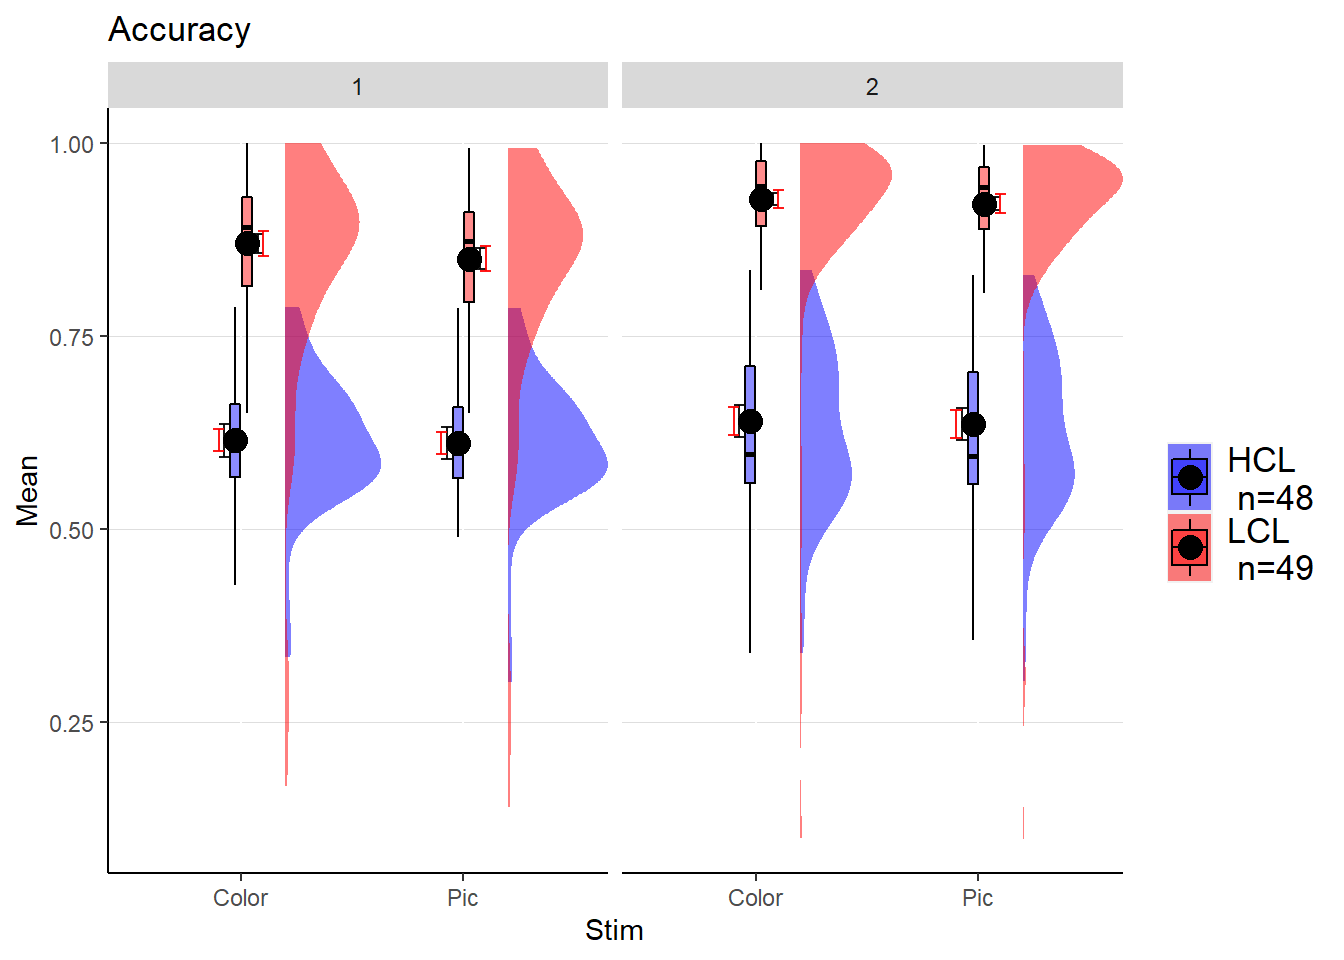
\includegraphics{ALL_TOGETHER_files/figure-latex/Performance-11}

\begin{Shaded}
\begin{Highlighting}[]
\NormalTok{two\_w }\OtherTok{\textless{}{-}} \FunctionTok{glmer}\NormalTok{(Mean }\SpecialCharTok{\textasciitilde{}}\NormalTok{ Time }\SpecialCharTok{*}\NormalTok{ Stim }\SpecialCharTok{+}\NormalTok{ (}\DecValTok{1} \SpecialCharTok{|}\NormalTok{ ID), }\AttributeTok{weights =}\NormalTok{ count,}
   \AttributeTok{family =}\NormalTok{ binomial, }\AttributeTok{data =}\NormalTok{ EXP1)}
\NormalTok{emmeans1}\OtherTok{\textless{}{-}} \FunctionTok{emmeans}\NormalTok{(two\_w, pairwise }\SpecialCharTok{\textasciitilde{}}\NormalTok{ Time }\SpecialCharTok{*}\NormalTok{ Stim, }\AttributeTok{adjust =}\StringTok{"fdr"}\NormalTok{, }\AttributeTok{type =} \StringTok{"response"}\NormalTok{)}
\NormalTok{emmean\_dataframe }\OtherTok{\textless{}{-}} \FunctionTok{summary}\NormalTok{(emmeans1)}\SpecialCharTok{$}\NormalTok{emmeans}

\FunctionTok{Anova}\NormalTok{(three\_w, }\AttributeTok{type=}\StringTok{\textquotesingle{}III\textquotesingle{}}\NormalTok{)}
\end{Highlighting}
\end{Shaded}

\begin{verbatim}
## Analysis of Deviance Table (Type III Wald chisquare tests)
## 
## Response: Mean
##                        Chisq Df Pr(>Chisq)    
## (Intercept)          27.5233  1  1.552e-07 ***
## Condition           107.5407  1  < 2.2e-16 ***
## Time                  8.6023  1   0.003357 ** 
## Stim                  0.1552  1   0.693569    
## Condition:Time       26.2623  1  2.981e-07 ***
## Condition:Stim        2.5317  1   0.111578    
## Time:Stim             0.0014  1   0.970086    
## Condition:Time:Stim   0.2982  1   0.585018    
## ---
## Signif. codes:  0 '***' 0.001 '**' 0.01 '*' 0.05 '.' 0.1 ' ' 1
\end{verbatim}

\begin{Shaded}
\begin{Highlighting}[]
\FunctionTok{summary}\NormalTok{(emmeans1)}
\end{Highlighting}
\end{Shaded}

\begin{verbatim}
## $emmeans
##  Time Stim   prob     SE  df asymp.LCL asymp.UCL
##  1    Color 0.777 0.0185 Inf     0.739     0.812
##  2    Color 0.806 0.0168 Inf     0.771     0.837
##  1    Pic   0.771 0.0189 Inf     0.732     0.806
##  2    Pic   0.802 0.0170 Inf     0.767     0.833
## 
## Confidence level used: 0.95 
## Intervals are back-transformed from the logit scale 
## 
## $contrasts
##  contrast          odds.ratio     SE  df null z.ratio p.value
##  1 Color / 2 Color      0.841 0.0288 Inf    1  -5.048  <.0001
##  1 Color / 1 Pic        1.038 0.0351 Inf    1   1.114  0.3182
##  1 Color / 2 Pic        0.862 0.0294 Inf    1  -4.357  <.0001
##  2 Color / 1 Pic        1.234 0.0420 Inf    1   6.173  <.0001
##  2 Color / 2 Pic        1.024 0.0352 Inf    1   0.690  0.4901
##  1 Pic / 2 Pic          0.830 0.0283 Inf    1  -5.480  <.0001
## 
## P value adjustment: fdr method for 6 tests 
## Tests are performed on the log odds ratio scale
\end{verbatim}

\begin{Shaded}
\begin{Highlighting}[]
\CommentTok{\# summary}
\NormalTok{sum }\OtherTok{\textless{}{-}} \FunctionTok{sum\_2}\NormalTok{ (EXP1, }\StringTok{\textquotesingle{}Stim\textquotesingle{}}\NormalTok{, }\StringTok{\textquotesingle{}Condition\textquotesingle{}}\NormalTok{, }\StringTok{\textquotesingle{}Mean\textquotesingle{}}\NormalTok{)}
\NormalTok{sum}
\end{Highlighting}
\end{Shaded}

\begin{verbatim}
## # A tibble: 4 x 7
## # Groups:   Stim [2]
##   Stim  Condition     n  mean     sd      se     ic
##   <fct> <fct>     <int> <dbl>  <dbl>   <dbl>  <dbl>
## 1 Color HCL         192 0.623 0.0917 0.00662 0.0130
## 2 Color LCL         196 0.875 0.153  0.0109  0.0215
## 3 Pic   HCL         192 0.619 0.0923 0.00666 0.0131
## 4 Pic   LCL         196 0.863 0.154  0.0110  0.0217
\end{verbatim}

\begin{Shaded}
\begin{Highlighting}[]
\NormalTok{pl }\OtherTok{\textless{}{-}} \FunctionTok{plotti}\NormalTok{(EXP1, emmean\_dataframe, }\StringTok{\textquotesingle{}Stim\textquotesingle{}}\NormalTok{, }\StringTok{\textquotesingle{}Mean\textquotesingle{}}\NormalTok{, }\StringTok{\textquotesingle{}Time\textquotesingle{}}\NormalTok{, }\StringTok{\textquotesingle{}prob\textquotesingle{}}\NormalTok{, }\StringTok{\textquotesingle{}Stimulus\textquotesingle{}}\NormalTok{)}
\end{Highlighting}
\end{Shaded}

\begin{center}\rule{0.5\linewidth}{0.5pt}\end{center}

\hypertarget{correlations}{%
\subsection{CORRELATIONS}\label{correlations}}

\begin{Shaded}
\begin{Highlighting}[]
\DocumentationTok{\#\#\#\#\#\#\#\#\#\#\#\#\#\#\#\#\#\#\#\#\#\#\#\#\#\#\#\#\#\#\#\#\#\#\#\#\#\#\#\#\#\#}
  \DocumentationTok{\#\#\# CORRELATIONS }\AlertTok{\#\#\#}
\DocumentationTok{\#\#\#\#\#\#\#\#\#\#\#\#\#\#\#\#\#\#\#\#\#\#\#\#\#\#\#\#\#\#\#\#\#\#\#\#\#\#\#\#\#C}

 \CommentTok{\# Create 1 big dataframe}
 \FunctionTok{names}\NormalTok{(VAS)[}\FunctionTok{names}\NormalTok{(VAS)}\SpecialCharTok{==}\StringTok{"Mean"}\NormalTok{] }\OtherTok{\textless{}{-}} \StringTok{"VASf"}
 \FunctionTok{names}\NormalTok{(EXP)[}\FunctionTok{names}\NormalTok{(EXP)}\SpecialCharTok{==}\StringTok{"Mean"}\NormalTok{] }\OtherTok{\textless{}{-}} \StringTok{"Acc"}
\NormalTok{ df }\OtherTok{\textless{}{-}} \FunctionTok{merge}\NormalTok{(VAS, EXP, }\AttributeTok{by =} \FunctionTok{c}\NormalTok{(}\StringTok{\textquotesingle{}Day\textquotesingle{}}\NormalTok{,}\StringTok{\textquotesingle{}Time\textquotesingle{}}\NormalTok{, }\StringTok{\textquotesingle{}Condition\textquotesingle{}}\NormalTok{, }\StringTok{\textquotesingle{}ID\textquotesingle{}}\NormalTok{))}

 \FunctionTok{length}\NormalTok{(}\FunctionTok{unique}\NormalTok{(df}\SpecialCharTok{$}\NormalTok{ID[df}\SpecialCharTok{$}\NormalTok{Condition}\SpecialCharTok{==}\StringTok{\textquotesingle{}HCL\textquotesingle{}}\NormalTok{]))}
\end{Highlighting}
\end{Shaded}

\begin{verbatim}
## [1] 48
\end{verbatim}

\begin{Shaded}
\begin{Highlighting}[]
 \FunctionTok{length}\NormalTok{(}\FunctionTok{unique}\NormalTok{(df}\SpecialCharTok{$}\NormalTok{ID[df}\SpecialCharTok{$}\NormalTok{Condition}\SpecialCharTok{==}\StringTok{\textquotesingle{}LCL\textquotesingle{}}\NormalTok{]))}
\end{Highlighting}
\end{Shaded}

\begin{verbatim}
## [1] 48
\end{verbatim}

\begin{Shaded}
\begin{Highlighting}[]
 \DocumentationTok{\#\#\# VAS{-}f }\AlertTok{\#\#\#}

 \DocumentationTok{\#\# CORR VAS{-}f Mean score between Day 1 and Day 2 (test{-}retest reliability)}
 \CommentTok{\# HCL}
\NormalTok{ Day1 }\OtherTok{\textless{}{-}}\NormalTok{ VAS}\SpecialCharTok{$}\NormalTok{VASf[VAS}\SpecialCharTok{$}\NormalTok{Day}\SpecialCharTok{==}\DecValTok{1} \SpecialCharTok{\&}\NormalTok{ VAS}\SpecialCharTok{$}\NormalTok{Condition}\SpecialCharTok{==}\StringTok{\textquotesingle{}HCL\textquotesingle{}}\NormalTok{]}
\NormalTok{ Day2 }\OtherTok{\textless{}{-}}\NormalTok{ VAS}\SpecialCharTok{$}\NormalTok{VASf[VAS}\SpecialCharTok{$}\NormalTok{Day}\SpecialCharTok{==}\DecValTok{2} \SpecialCharTok{\&}\NormalTok{ VAS}\SpecialCharTok{$}\NormalTok{Condition}\SpecialCharTok{==}\StringTok{\textquotesingle{}HCL\textquotesingle{}}\NormalTok{]}
\NormalTok{ VASfHCL }\OtherTok{\textless{}{-}} \FunctionTok{corrplot}\NormalTok{(Day1, Day2, }\StringTok{\textquotesingle{}Day1\textquotesingle{}}\NormalTok{, }\StringTok{\textquotesingle{}Day2\textquotesingle{}}\NormalTok{) }\SpecialCharTok{+}\FunctionTok{ggtitle}\NormalTok{(}\StringTok{\textquotesingle{}VASf HCL\textquotesingle{}}\NormalTok{)}
 \CommentTok{\#LCL}
\NormalTok{ Day1 }\OtherTok{\textless{}{-}}\NormalTok{ VAS}\SpecialCharTok{$}\NormalTok{VASf[VAS}\SpecialCharTok{$}\NormalTok{Day}\SpecialCharTok{==}\DecValTok{1} \SpecialCharTok{\&}\NormalTok{ VAS}\SpecialCharTok{$}\NormalTok{Condition}\SpecialCharTok{==}\StringTok{\textquotesingle{}LCL\textquotesingle{}}\NormalTok{]}
\NormalTok{ Day2 }\OtherTok{\textless{}{-}}\NormalTok{ VAS}\SpecialCharTok{$}\NormalTok{VASf[VAS}\SpecialCharTok{$}\NormalTok{Day}\SpecialCharTok{==}\DecValTok{2} \SpecialCharTok{\&}\NormalTok{ VAS}\SpecialCharTok{$}\NormalTok{Condition}\SpecialCharTok{==}\StringTok{\textquotesingle{}LCL\textquotesingle{}}\NormalTok{]}
\NormalTok{ VASfLCL }\OtherTok{\textless{}{-}} \FunctionTok{corrplot}\NormalTok{(Day1, Day2, }\StringTok{\textquotesingle{}Day1\textquotesingle{}}\NormalTok{, }\StringTok{\textquotesingle{}Day2\textquotesingle{}}\NormalTok{) }\SpecialCharTok{+}\FunctionTok{ggtitle}\NormalTok{(}\StringTok{\textquotesingle{}VASf LCL\textquotesingle{}}\NormalTok{)}
 \CommentTok{\# cor.test(VAS$VASf[VAS$Condition==\textquotesingle{}HCL\textquotesingle{}], VAS$VASf[VAS$Condition==\textquotesingle{}LCL\textquotesingle{}],  method="spearman")\# not Pearson because: not normal distribution}
 \CommentTok{\# cor.test(VAS$Mean[VAS$Condition==\textquotesingle{}HCL\textquotesingle{}], VAS$Mean[VAS$Condition==\textquotesingle{}LCL\textquotesingle{}],  method="kendall")}

 \DocumentationTok{\#\# CORR VAS{-}f delta between Day 1 and Day 2}
 \CommentTok{\#HCL}
\NormalTok{ Day1 }\OtherTok{\textless{}{-}}\NormalTok{ VAS}\SpecialCharTok{$}\NormalTok{VASf[VAS}\SpecialCharTok{$}\NormalTok{Day}\SpecialCharTok{==}\DecValTok{1} \SpecialCharTok{\&}\NormalTok{ VAS}\SpecialCharTok{$}\NormalTok{Condition}\SpecialCharTok{==}\StringTok{\textquotesingle{}HCL\textquotesingle{}} \SpecialCharTok{\&}\NormalTok{ VAS}\SpecialCharTok{$}\NormalTok{Time}\SpecialCharTok{==}\DecValTok{2}\NormalTok{]}\SpecialCharTok{{-}}\NormalTok{ VAS}\SpecialCharTok{$}\NormalTok{VASf[VAS}\SpecialCharTok{$}\NormalTok{Day}\SpecialCharTok{==}\DecValTok{1} \SpecialCharTok{\&}\NormalTok{ VAS}\SpecialCharTok{$}\NormalTok{Condition}\SpecialCharTok{==}\StringTok{\textquotesingle{}HCL\textquotesingle{}} \SpecialCharTok{\&}\NormalTok{ VAS}\SpecialCharTok{$}\NormalTok{Time}\SpecialCharTok{==}\DecValTok{1}\NormalTok{]}
\NormalTok{ Day2 }\OtherTok{\textless{}{-}}\NormalTok{ VAS}\SpecialCharTok{$}\NormalTok{VASf[VAS}\SpecialCharTok{$}\NormalTok{Day}\SpecialCharTok{==}\DecValTok{2} \SpecialCharTok{\&}\NormalTok{ VAS}\SpecialCharTok{$}\NormalTok{Condition}\SpecialCharTok{==}\StringTok{\textquotesingle{}HCL\textquotesingle{}} \SpecialCharTok{\&}\NormalTok{ VAS}\SpecialCharTok{$}\NormalTok{Time}\SpecialCharTok{==}\DecValTok{2}\NormalTok{]}\SpecialCharTok{{-}}\NormalTok{ VAS}\SpecialCharTok{$}\NormalTok{VASf[VAS}\SpecialCharTok{$}\NormalTok{Day}\SpecialCharTok{==}\DecValTok{2} \SpecialCharTok{\&}\NormalTok{ VAS}\SpecialCharTok{$}\NormalTok{Condition}\SpecialCharTok{==}\StringTok{\textquotesingle{}HCL\textquotesingle{}} \SpecialCharTok{\&}\NormalTok{ VAS}\SpecialCharTok{$}\NormalTok{Time}\SpecialCharTok{==}\DecValTok{1}\NormalTok{]}
\NormalTok{ VASf\_delta\_HCL }\OtherTok{\textless{}{-}} \FunctionTok{corrplot}\NormalTok{(Day1, Day2, }\StringTok{\textquotesingle{}Day1\textquotesingle{}}\NormalTok{, }\StringTok{\textquotesingle{}Day2\textquotesingle{}}\NormalTok{) }\SpecialCharTok{+}\FunctionTok{ggtitle}\NormalTok{(}\StringTok{\textquotesingle{}VASf delta HCL\textquotesingle{}}\NormalTok{)}
 \CommentTok{\#LCL}
\NormalTok{ Day1 }\OtherTok{\textless{}{-}}\NormalTok{ VAS}\SpecialCharTok{$}\NormalTok{VASf[VAS}\SpecialCharTok{$}\NormalTok{Day}\SpecialCharTok{==}\DecValTok{1} \SpecialCharTok{\&}\NormalTok{ VAS}\SpecialCharTok{$}\NormalTok{Condition}\SpecialCharTok{==}\StringTok{\textquotesingle{}LCL\textquotesingle{}} \SpecialCharTok{\&}\NormalTok{ VAS}\SpecialCharTok{$}\NormalTok{Time}\SpecialCharTok{==}\DecValTok{2}\NormalTok{]}\SpecialCharTok{{-}}\NormalTok{ VAS}\SpecialCharTok{$}\NormalTok{VASf[VAS}\SpecialCharTok{$}\NormalTok{Day}\SpecialCharTok{==}\DecValTok{1} \SpecialCharTok{\&}\NormalTok{ VAS}\SpecialCharTok{$}\NormalTok{Condition}\SpecialCharTok{==}\StringTok{\textquotesingle{}LCL\textquotesingle{}} \SpecialCharTok{\&}\NormalTok{ VAS}\SpecialCharTok{$}\NormalTok{Time}\SpecialCharTok{==}\DecValTok{1}\NormalTok{]}
\NormalTok{ Day2 }\OtherTok{\textless{}{-}}\NormalTok{ VAS}\SpecialCharTok{$}\NormalTok{VASf[VAS}\SpecialCharTok{$}\NormalTok{Day}\SpecialCharTok{==}\DecValTok{2} \SpecialCharTok{\&}\NormalTok{ VAS}\SpecialCharTok{$}\NormalTok{Condition}\SpecialCharTok{==}\StringTok{\textquotesingle{}LCL\textquotesingle{}} \SpecialCharTok{\&}\NormalTok{ VAS}\SpecialCharTok{$}\NormalTok{Time}\SpecialCharTok{==}\DecValTok{2}\NormalTok{]}\SpecialCharTok{{-}}\NormalTok{ VAS}\SpecialCharTok{$}\NormalTok{VASf[VAS}\SpecialCharTok{$}\NormalTok{Day}\SpecialCharTok{==}\DecValTok{2} \SpecialCharTok{\&}\NormalTok{ VAS}\SpecialCharTok{$}\NormalTok{Condition}\SpecialCharTok{==}\StringTok{\textquotesingle{}LCL\textquotesingle{}} \SpecialCharTok{\&}\NormalTok{ VAS}\SpecialCharTok{$}\NormalTok{Time}\SpecialCharTok{==}\DecValTok{1}\NormalTok{]}
\NormalTok{ VASf\_delta\_LCL }\OtherTok{\textless{}{-}} \FunctionTok{corrplot}\NormalTok{(Day1, Day2, }\StringTok{\textquotesingle{}Day1\textquotesingle{}}\NormalTok{, }\StringTok{\textquotesingle{}Day2\textquotesingle{}}\NormalTok{) }\SpecialCharTok{+}\FunctionTok{ggtitle}\NormalTok{(}\StringTok{\textquotesingle{}VASf delta LCL\textquotesingle{}}\NormalTok{)}

\NormalTok{ VASfCORR }\OtherTok{\textless{}{-}} \FunctionTok{ggarrange}\NormalTok{(VASfHCL, VASfLCL, VASf\_delta\_HCL, VASf\_delta\_LCL }\SpecialCharTok{+} \FunctionTok{rremove}\NormalTok{(}\StringTok{"x.text"}\NormalTok{),}
           \AttributeTok{labels =} \FunctionTok{c}\NormalTok{(}\StringTok{"A"}\NormalTok{, }\StringTok{"B"}\NormalTok{, }\StringTok{"C"}\NormalTok{, }\StringTok{"D"}\NormalTok{),}
           \AttributeTok{ncol =} \DecValTok{2}\NormalTok{, }\AttributeTok{nrow =} \DecValTok{2}\NormalTok{)}
 \FunctionTok{ggsave}\NormalTok{(VASfCORR, }\AttributeTok{file=}\FunctionTok{paste0}\NormalTok{(plotPrefix, }\StringTok{"VASf\_CORR.jpg"}\NormalTok{), }\AttributeTok{width =} \DecValTok{2500}\NormalTok{, }\AttributeTok{height =} \DecValTok{1500}\NormalTok{, }\AttributeTok{dpi =} \DecValTok{300}\NormalTok{, }\AttributeTok{units =} \StringTok{"px"}\NormalTok{)}
\NormalTok{ VASfCORR}
\end{Highlighting}
\end{Shaded}

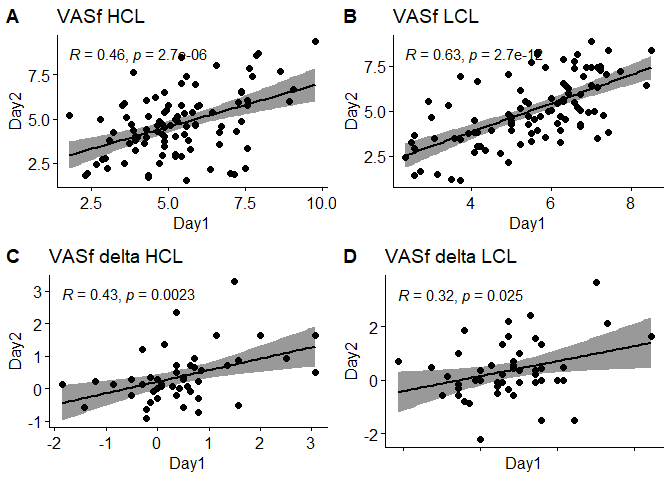
\includegraphics{ALL_TOGETHER_files/figure-latex/unnamed-chunk-1-1}

\begin{Shaded}
\begin{Highlighting}[]
 \DocumentationTok{\#\#\# Accuracy }\AlertTok{\#\#\#}
\CommentTok{\# }
\CommentTok{\#  \#\# CORR Accuracy Day 1 and Day 2  (test{-}retest reliability)}
\CommentTok{\#  \#HCL}
\CommentTok{\#  EXP \textless{}{-} EXP[!(EXP$ID==49),]}
\CommentTok{\#  Day1 \textless{}{-} EXP$Acc[EXP$Day==1 \& EXP$Condition==\textquotesingle{}HCL\textquotesingle{} \& EXP$Time==2]{-} EXP$Acc[EXP$Day==1 \& EXP$Condition==\textquotesingle{}HCL\textquotesingle{} \& EXP$Time==1]}
\CommentTok{\#  Day2 \textless{}{-} EXP$Acc[EXP$Day==2 \& EXP$Condition==\textquotesingle{}HCL\textquotesingle{} \& EXP$Time==2]{-} EXP$Acc[EXP$Day==2 \& EXP$Condition==\textquotesingle{}HCL\textquotesingle{} \& EXP$Time==1]}
\CommentTok{\#  EXPHCL\textless{}{-}corrplot(Day1, Day2, \textquotesingle{}Day1\textquotesingle{}, \textquotesingle{}Day2\textquotesingle{}) +ggtitle(\textquotesingle{}Performance HCL\textquotesingle{})}
\CommentTok{\#  \#LCL}
\CommentTok{\#  Day1 \textless{}{-} EXP$Acc[EXP$Day==1 \& EXP$Condition==\textquotesingle{}LCL\textquotesingle{} \& EXP$Time==2]{-} EXP$Acc[EXP$Day==1 \& EXP$Condition==\textquotesingle{}LCL\textquotesingle{} \& EXP$Time==1]}
\CommentTok{\#  Day2 \textless{}{-} EXP$Acc[EXP$Day==2 \& EXP$Condition==\textquotesingle{}LCL\textquotesingle{} \& EXP$Time==2]{-} EXP$Acc[EXP$Day==2 \& EXP$Condition==\textquotesingle{}LCL\textquotesingle{} \& EXP$Time==1]}
\CommentTok{\#  EXPLCL\textless{}{-}corrplot(Day1, Day2, \textquotesingle{}Day1\textquotesingle{}, \textquotesingle{}Day2\textquotesingle{}) +ggtitle(\textquotesingle{}Performance LCL\textquotesingle{})}
\CommentTok{\# }
\CommentTok{\#  \#\# CORR Accuracy delta between Day 1 and Day 2}
\CommentTok{\#  \#HCL}
\CommentTok{\#  Day1 \textless{}{-} EXP$Acc[EXP$Day==1 \& EXP$Condition==\textquotesingle{}HCL\textquotesingle{} \& EXP$Time==2]{-} EXP$Acc[EXP$Day==1 \& EXP$Condition==\textquotesingle{}HCL\textquotesingle{} \& EXP$Time==1]}
\CommentTok{\#  Day2 \textless{}{-} EXP$Acc[EXP$Day==2 \& EXP$Condition==\textquotesingle{}HCL\textquotesingle{} \& EXP$Time==2]{-} EXP$Acc[EXP$Day==2 \& EXP$Condition==\textquotesingle{}HCL\textquotesingle{} \& EXP$Time==1]}
\CommentTok{\#  EXP\_DELTA\_HCL\textless{}{-} corrplot(Day1, Day2, \textquotesingle{}Day1\textquotesingle{}, \textquotesingle{}Day2\textquotesingle{}) +ggtitle(\textquotesingle{}Performance delta HCL\textquotesingle{}) \# negative correlation: when high in day 1, low in day 2}
\CommentTok{\#  \#LCL}
\CommentTok{\#  Day1 \textless{}{-} EXP$Acc[EXP$Day==1 \& EXP$Condition==\textquotesingle{}LCL\textquotesingle{} \& EXP$Time==2]{-} EXP$Acc[EXP$Day==1 \& EXP$Condition==\textquotesingle{}LCL\textquotesingle{} \& EXP$Time==1]}
\CommentTok{\#  Day2 \textless{}{-} EXP$Acc[EXP$Day==2 \& EXP$Condition==\textquotesingle{}LCL\textquotesingle{} \& EXP$Time==2]{-} EXP$Acc[EXP$Day==2 \& EXP$Condition==\textquotesingle{}LCL\textquotesingle{} \& EXP$Time==1]}
\CommentTok{\#  EXP\_DELTA\_LCL\textless{}{-}corrplot(Day1, Day2, \textquotesingle{}Day1\textquotesingle{}, \textquotesingle{}Day2\textquotesingle{}) +ggtitle(\textquotesingle{}Performance delta LCL\textquotesingle{}) \# positive correlation: when high in day 1, high in day 2}
\CommentTok{\# }
\CommentTok{\#  EXPCORR \textless{}{-} ggarrange(EXPHCL, EXPLCL, EXP\_DELTA\_HCL, EXP\_DELTA\_LCL + rremove("x.text"),}
\CommentTok{\#            labels = c("A", "B", "C", "D"),}
\CommentTok{\#            ncol = 2, nrow = 2)}
\CommentTok{\#  ggsave(EXPCORR, file=paste0(plotPrefix, "EXP\_CORR.jpg"), width = 2500, height = 1500, dpi = 300, units = "px")}
\CommentTok{\#  EXPCORR}

 \DocumentationTok{\#\#\# VAS{-}f * Acc }\AlertTok{\#\#\#}
 \DocumentationTok{\#\# CORR delta (change) VAS{-}f and delta Acc}
 \CommentTok{\#HCL}
\NormalTok{ VAS\_f }\OtherTok{\textless{}{-}}\NormalTok{ df}\SpecialCharTok{$}\NormalTok{VASf[df}\SpecialCharTok{$}\NormalTok{Time}\SpecialCharTok{==}\DecValTok{2} \SpecialCharTok{\&}\NormalTok{ df}\SpecialCharTok{$}\NormalTok{Condition}\SpecialCharTok{==}\StringTok{\textquotesingle{}HCL\textquotesingle{}}\NormalTok{] }\SpecialCharTok{{-}}\NormalTok{ df}\SpecialCharTok{$}\NormalTok{VASf[df}\SpecialCharTok{$}\NormalTok{Time}\SpecialCharTok{==}\DecValTok{1} \SpecialCharTok{\&}\NormalTok{ df}\SpecialCharTok{$}\NormalTok{Condition}\SpecialCharTok{==}\StringTok{\textquotesingle{}HCL\textquotesingle{}}\NormalTok{]}
\NormalTok{ ACC}\OtherTok{\textless{}{-}}\NormalTok{ df}\SpecialCharTok{$}\NormalTok{Acc[df}\SpecialCharTok{$}\NormalTok{Time}\SpecialCharTok{==}\DecValTok{2} \SpecialCharTok{\&}\NormalTok{ df}\SpecialCharTok{$}\NormalTok{Condition}\SpecialCharTok{==}\StringTok{\textquotesingle{}HCL\textquotesingle{}}\NormalTok{] }\SpecialCharTok{{-}}\NormalTok{ df}\SpecialCharTok{$}\NormalTok{Acc[df}\SpecialCharTok{$}\NormalTok{Time}\SpecialCharTok{==}\DecValTok{1} \SpecialCharTok{\&}\NormalTok{ df}\SpecialCharTok{$}\NormalTok{Condition}\SpecialCharTok{==}\StringTok{\textquotesingle{}HCL\textquotesingle{}}\NormalTok{]}
\NormalTok{ DELTAHCL}\OtherTok{\textless{}{-}} \FunctionTok{corrplot}\NormalTok{(VAS\_f, ACC, }\StringTok{\textquotesingle{}VASf delta\textquotesingle{}}\NormalTok{, }\StringTok{\textquotesingle{}Performance delta\textquotesingle{}}\NormalTok{) }\SpecialCharTok{+}\FunctionTok{ggtitle}\NormalTok{(}\StringTok{\textquotesingle{}delta correlations HCL\textquotesingle{}}\NormalTok{) }\CommentTok{\# no correlation: change before{-}after test in VASf no correlation with obj CF changes}
 \CommentTok{\#LCL}
\NormalTok{ VAS\_f }\OtherTok{\textless{}{-}}\NormalTok{ df}\SpecialCharTok{$}\NormalTok{VASf[df}\SpecialCharTok{$}\NormalTok{Time}\SpecialCharTok{==}\DecValTok{2} \SpecialCharTok{\&}\NormalTok{ df}\SpecialCharTok{$}\NormalTok{Condition}\SpecialCharTok{==}\StringTok{\textquotesingle{}LCL\textquotesingle{}}\NormalTok{] }\SpecialCharTok{{-}}\NormalTok{ df}\SpecialCharTok{$}\NormalTok{VASf[df}\SpecialCharTok{$}\NormalTok{Time}\SpecialCharTok{==}\DecValTok{1} \SpecialCharTok{\&}\NormalTok{ df}\SpecialCharTok{$}\NormalTok{Condition}\SpecialCharTok{==}\StringTok{\textquotesingle{}LCL\textquotesingle{}}\NormalTok{]}
\NormalTok{ ACC}\OtherTok{\textless{}{-}}\NormalTok{ df}\SpecialCharTok{$}\NormalTok{Acc[df}\SpecialCharTok{$}\NormalTok{Time}\SpecialCharTok{==}\DecValTok{2} \SpecialCharTok{\&}\NormalTok{ df}\SpecialCharTok{$}\NormalTok{Condition}\SpecialCharTok{==}\StringTok{\textquotesingle{}LCL\textquotesingle{}}\NormalTok{] }\SpecialCharTok{{-}}\NormalTok{ df}\SpecialCharTok{$}\NormalTok{Acc[df}\SpecialCharTok{$}\NormalTok{Time}\SpecialCharTok{==}\DecValTok{1} \SpecialCharTok{\&}\NormalTok{ df}\SpecialCharTok{$}\NormalTok{Condition}\SpecialCharTok{==}\StringTok{\textquotesingle{}LCL\textquotesingle{}}\NormalTok{]}
\NormalTok{ DELTALCL}\OtherTok{\textless{}{-}} \FunctionTok{corrplot}\NormalTok{(VAS\_f, ACC, }\StringTok{\textquotesingle{}VASf delta\textquotesingle{}}\NormalTok{, }\StringTok{\textquotesingle{}Performance delta\textquotesingle{}}\NormalTok{) }\SpecialCharTok{+}\FunctionTok{ggtitle}\NormalTok{(}\StringTok{\textquotesingle{}delta correlations LCL\textquotesingle{}}\NormalTok{)}

\NormalTok{ DELTACORR}\OtherTok{\textless{}{-}} \FunctionTok{ggarrange}\NormalTok{ (DELTAHCL, DELTALCL}\SpecialCharTok{+} \FunctionTok{rremove}\NormalTok{(}\StringTok{\textquotesingle{}x.text\textquotesingle{}}\NormalTok{), }\AttributeTok{labels=} \FunctionTok{c}\NormalTok{(}\StringTok{\textquotesingle{}A\textquotesingle{}}\NormalTok{, }\StringTok{\textquotesingle{}B\textquotesingle{}}\NormalTok{))}
 \FunctionTok{ggsave}\NormalTok{(DELTACORR, }\AttributeTok{file=}\FunctionTok{paste0}\NormalTok{(plotPrefix, }\StringTok{"DELAT\_CORR.jpg"}\NormalTok{), }\AttributeTok{width =} \DecValTok{2500}\NormalTok{, }\AttributeTok{height =} \DecValTok{1500}\NormalTok{, }\AttributeTok{dpi =} \DecValTok{300}\NormalTok{, }\AttributeTok{units =} \StringTok{"px"}\NormalTok{)}
\NormalTok{ DELTACORR}
\end{Highlighting}
\end{Shaded}

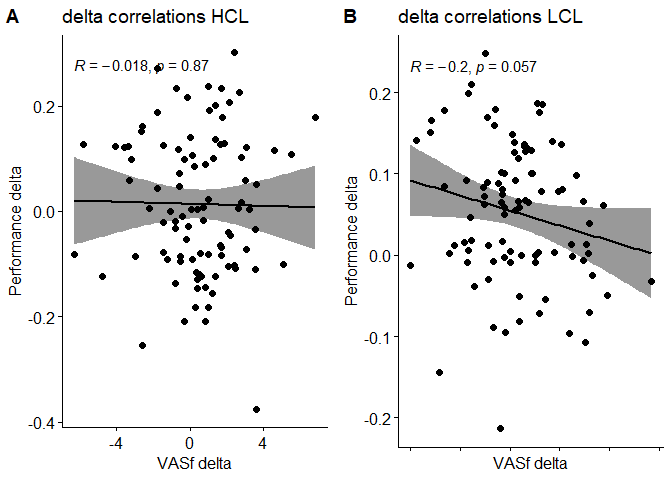
\includegraphics{ALL_TOGETHER_files/figure-latex/unnamed-chunk-1-2}

\end{document}
